%%=============================================================================
%% LaTeX sjabloon voor bachelorproef, HoGent Bedrijf en Organisatie
%% Opleiding Toegepaste Informatica
%%=============================================================================

\documentclass[fleqn,a4paper,12pt]{book}

%%=============================================================================
%% LaTeX sjabloon voor de bachelorproef, HoGent Bedrijf en Organisatie
%% Opleiding toegepaste informatica
%%
%% Structuur en algemene vormgeving. Meestal hoef je hier niets te wijzigen.
%%
%% Vormgeving gebaseerd op "The Legrand Orange Book", version 2.0 (9/2/15)
%% door Mathias Legrand (legrand.mathias@gmail.com) met aanpassingen door
%% Vel (vel@latextemplates.com). Het oorspronkelijke template is te vinden op
%% http://www.LaTeXTemplates.com
%%
%% Aanpassingen voor HoGent toegepaste informatica: 
%%   Bert Van Vreckem <bert.vanvreckem@hogent.be>
%% Licentie: 
%%   CC BY-NC-SA 3.0 (http://creativecommons.org/licenses/by-nc-sa/3.0/)
%%=============================================================================

%%-----------------------------------------------------------------------------
%% Packages
%%-----------------------------------------------------------------------------

\usepackage[top=3cm,bottom=3cm,left=3cm,right=3cm,headsep=10pt,a4paper]{geometry} % Page margins
\usepackage[utf8]{inputenc}  % Accenten gebruiken in tekst (vb. é ipv \'e)
\usepackage{amsfonts}        % AMS math packages: extra wiskundige
\usepackage{amsmath}         %   symbolen (o.a. getallen-
\usepackage{amssymb}         %   verzamelingen N, R, Z, Q, etc.)
\usepackage[english,dutch]{babel}    % Taalinstellingen: woordsplitsingen,
                             %  commando's voor speciale karakters
                             %  ("dutch" voor NL)
\usepackage{iflang}
\usepackage{eurosym}         % Euro-symbool €
\usepackage{geometry}
\usepackage{graphicx}        % Invoegen van tekeningen
\graphicspath{{img/}}       % Specifies the directory where pictures are stored
\usepackage{tikz}            % Required for drawing custom shapes
\usepackage[pdftex,bookmarks=true]{hyperref}
                             % PDF krijgt klikbare links & verwijzingen,
                             %  inhoudstafel
\usepackage{enumitem}        % Customize lists
\setlist{nolistsep}         % Reduce spacing between list items
\usepackage{listings}        % Broncode mooi opmaken
\usepackage{multirow}        % Tekst over verschillende cellen in tabellen
\usepackage{rotating}        % Tabellen en figuren roteren

\usepackage{booktabs}        % Required for nicer horizontal rules in tables

\usepackage{xcolor}          % Required for specifying colors by name
\definecolor{maincolor}{RGB}{0,147,208} % Define the main color used for 
                             % highlighting throughout the book
                             % 0, 147, 208 = officiële kleur HoGent FBO

% Paragraph style: no indent, add space between paragraphs
\setlength{\parindent}{0em}
\setlength{\parskip}{1em}

\usepackage{etoolbox}
\usepackage{titling} % Macros for title, author, etc
\usepackage{lipsum}          % Voor vultekst (lorem ipsum)

%----------------------------------------------------------------------------------------
%	FONTS
%----------------------------------------------------------------------------------------

\usepackage{avant} % Use the Avantgarde font for headings
%\usepackage{times} % Use the Times font for headings
\usepackage{mathptmx} % Use the Adobe Times Roman as the default text font together with math symbols from the Sym­bol, Chancery and Com­puter Modern fonts

\usepackage{microtype} % Slightly tweak font spacing for aesthetics
\usepackage[utf8]{inputenc} % Required for including letters with accents
\usepackage[T1]{fontenc} % Use 8-bit encoding that has 256 glyphs

%------------------------------------------------------------------------------
%	TITLE PAGE
%------------------------------------------------------------------------------

\newcommand{\inserttitlepage}{%
\begin{titlepage}
  \newgeometry{top=2cm,bottom=1.5cm,left=1.5cm,right=1.5cm}
  \begin{center}

    \begingroup
    \rmfamily
    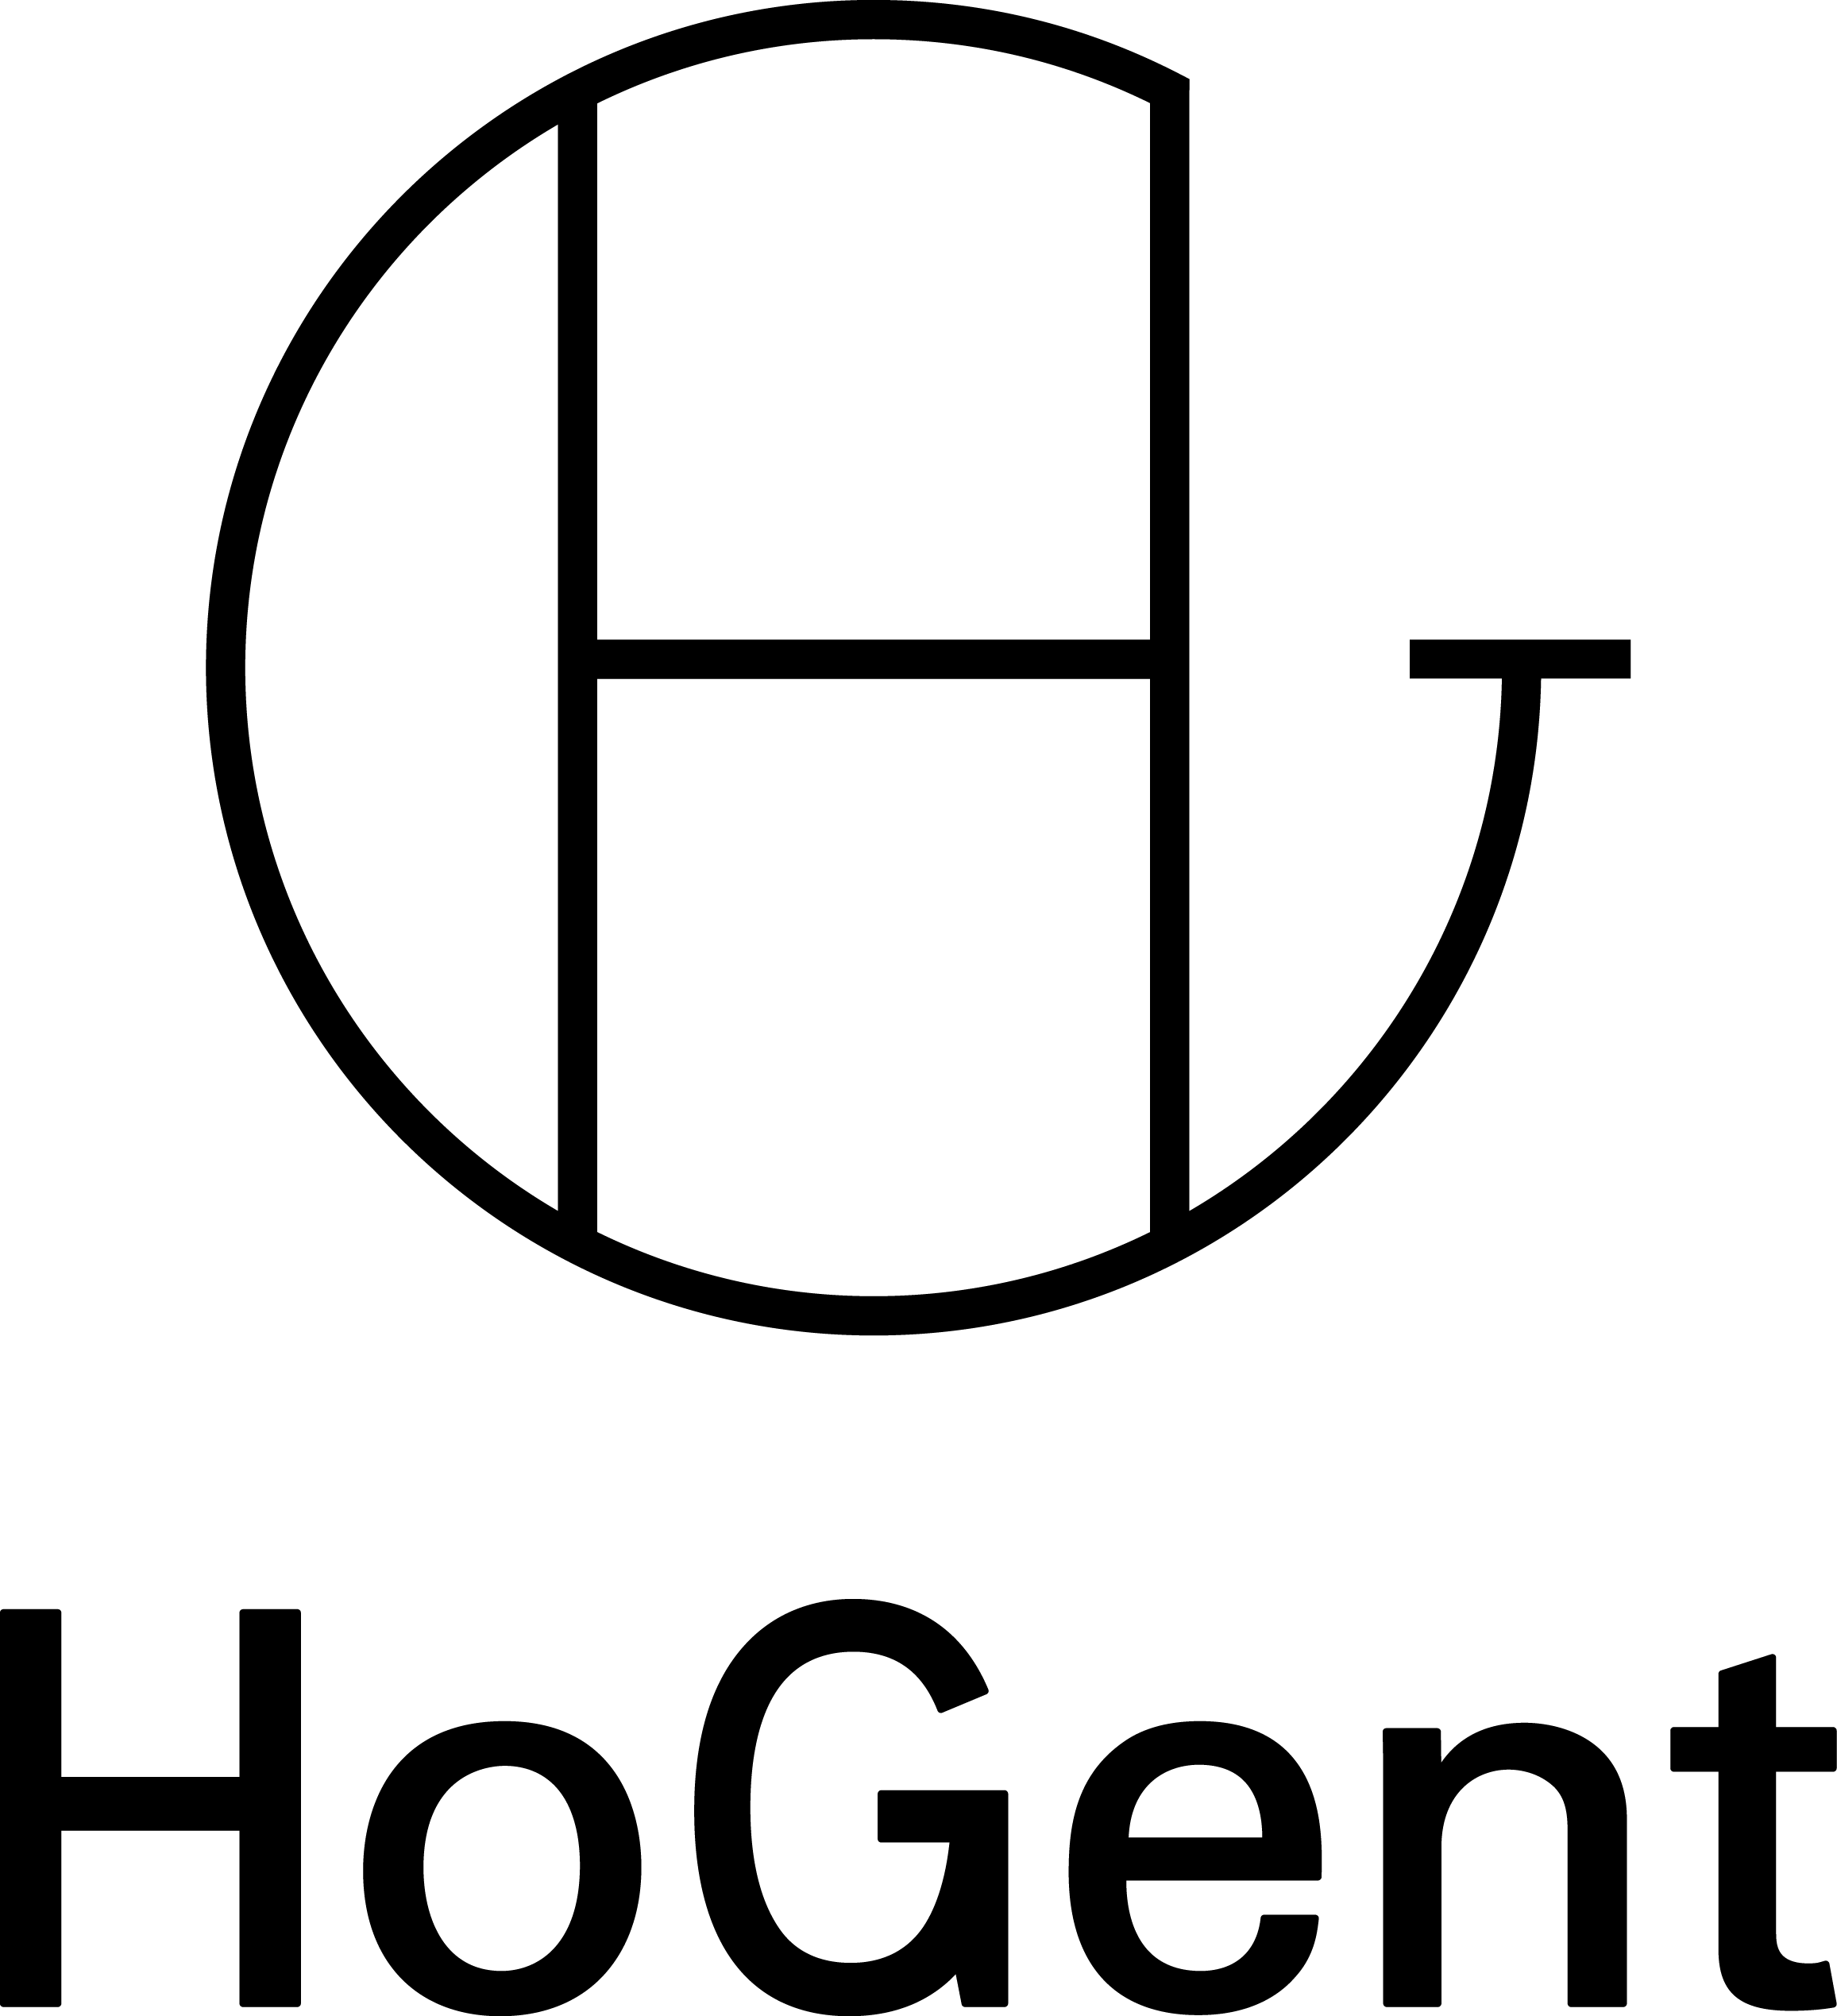
\includegraphics[width=2.5cm]{img/HG-beeldmerk-woordmerk}\\[.5cm]
    Faculteit Bedrijf en Organisatie\\[3cm]
    \titel
    \vfill
    \student\\[3.5cm]
    Scriptie voorgedragen tot het bekomen van de graad van\\professionele bachelor in de toegepaste informatica\\[2cm]
    Promotor:\\
    \promotor\\
    \ifdefempty{\copromotor}{\vspace{2.5cm}}{Co-promotor:\\\copromotor\\[2.5cm]}
    Instelling: \instelling\\[.5cm]
    Academiejaar: \academiejaar\\[.5cm]
    \ifcase \examenperiode \or Eerste \or Tweede \else Derde \fi examenperiode
    \endgroup

  \end{center}
  \restoregeometry
\end{titlepage}
  \emptypage
\begin{titlepage}
  \newgeometry{top=5.35cm,bottom=1.5cm,left=1.5cm,right=1.5cm}
  \begin{center}

    \begingroup
    \rmfamily
    \IfLanguageName{dutch}{Faculteit Bedrijf en Organisatie}{Faculty of Business and Information Management}\\[3cm]
    \titel
    \vfill
    \student\\[3.5cm]
    \IfLanguageName{dutch}{Scriptie voorgedragen tot het bekomen van de graad van\\professionele bachelor in de toegepaste informatica}{Thesis submitted in partial fulfilment of the requirements for the degree of\\professional bachelor of applied computer science}\\[2cm]
    Promotor:\\
    \promotor\\
    \ifdefempty{\copromotor}{\vspace{2.5cm}}{Co-promotor:\\\copromotor\\[2.5cm]}
    \IfLanguageName{dutch}{Instelling}{Institution}: \instelling\\[.5cm]
    \IfLanguageName{dutch}{Academiejaar}{Academic year}: \academiejaar\\[.5cm]
    \IfLanguageName{dutch}{%
    \ifcase \examenperiode \or Eerste \or Tweede \else Derde \fi examenperiode}{%
    \ifcase \examenperiode \or First \or Second \else Third \fi examination period}
    \endgroup

  \end{center}
  \restoregeometry
\end{titlepage}
}

%----------------------------------------------------------------------------------------
%	BIBLIOGRAPHY AND INDEX
%----------------------------------------------------------------------------------------

\usepackage[style=apa,backend=biber]{biblatex}
\usepackage{csquotes}
\DeclareLanguageMapping{dutch}{dutch-apa}
\addbibresource{bachproef-tin.bib} % BibTeX bibliography file
\addbibresource{../voorstel/voorstel.bib}
\defbibheading{bibempty}{}

\usepackage{calc} % For simpler calculation - used for spacing the index letter headings correctly
\usepackage{makeidx} % Required to make an index
\makeindex % Tells LaTeX to create the files required for indexing

%----------------------------------------------------------------------------------------
%	MAIN TABLE OF CONTENTS
%----------------------------------------------------------------------------------------

\usepackage{titletoc} % Required for manipulating the table of contents

\contentsmargin{0cm} % Removes the default margin

% Part text styling
\titlecontents{part}[0cm]
{\addvspace{20pt}\centering\large\bfseries}
{}
{}
{}

% Chapter text styling
\titlecontents{chapter}[1.25cm] % Indentation
{\addvspace{12pt}\large\sffamily\bfseries} % Spacing and font options for chapters
{\color{maincolor!60}\contentslabel[\Large\thecontentslabel]{1.25cm}\color{maincolor}} % Chapter number
{\color{maincolor}}
{\color{maincolor!60}\normalsize\;\titlerule*[.5pc]{.}\;\thecontentspage} % Page number

% Section text styling
\titlecontents{section}[1.25cm] % Indentation
{\addvspace{3pt}\sffamily\bfseries} % Spacing and font options for sections
{\contentslabel[\thecontentslabel]{1.25cm}} % Section number
{}
{\hfill\color{black}\thecontentspage} % Page number
[]

% Subsection text styling
\titlecontents{subsection}[1.25cm] % Indentation
{\addvspace{1pt}\sffamily\small} % Spacing and font options for subsections
{\contentslabel[\thecontentslabel]{1.25cm}} % Subsection number
{}
{\ \titlerule*[.5pc]{.}\;\thecontentspage} % Page number
[]

% List of figures
\titlecontents{figure}[0em]
{\addvspace{-5pt}\sffamily}
{\thecontentslabel\hspace*{1em}}
{}
{\ \titlerule*[.5pc]{.}\;\thecontentspage}
[]

% List of tables
\titlecontents{table}[0em]
{\addvspace{-5pt}\sffamily}
{\thecontentslabel\hspace*{1em}}
{}
{\ \titlerule*[.5pc]{.}\;\thecontentspage}
[]

%----------------------------------------------------------------------------------------
%	MINI TABLE OF CONTENTS IN PART HEADS
%----------------------------------------------------------------------------------------

% Chapter text styling
\titlecontents{lchapter}[0em] % Indenting
{\addvspace{15pt}\large\sffamily\bfseries} % Spacing and font options for chapters
{\color{maincolor}\contentslabel[\Large\thecontentslabel]{1.25cm}\color{maincolor}} % Chapter number
{}
{\color{maincolor}\normalsize\sffamily\bfseries\;\titlerule*[.5pc]{.}\;\thecontentspage} % Page number

% Section text styling
\titlecontents{lsection}[0em] % Indenting
{\sffamily\small} % Spacing and font options for sections
{\contentslabel[\thecontentslabel]{1.25cm}} % Section number
{}
{}

% Subsection text styling
\titlecontents{lsubsection}[.5em] % Indentation
{\normalfont\footnotesize\sffamily} % Font settings
{}
{}
{}

%----------------------------------------------------------------------------------------
%	PAGE HEADERS
%----------------------------------------------------------------------------------------

\usepackage{fancyhdr} % Required for header and footer configuration

\pagestyle{fancy}
\renewcommand{\chaptermark}[1]{\markboth{\sffamily\normalsize\bfseries\chaptername\ \thechapter.\ #1}{}} % Chapter text font settings
\renewcommand{\sectionmark}[1]{\markright{\sffamily\normalsize\thesection\hspace{5pt}#1}{}} % Section text font settings
\fancyhf{} \fancyhead[LE,RO]{\sffamily\normalsize\thepage} % Font setting for the page number in the header
\fancyhead[LO]{\rightmark} % Print the nearest section name on the left side of odd pages
\fancyhead[RE]{\leftmark} % Print the current chapter name on the right side of even pages
\renewcommand{\headrulewidth}{0.5pt} % Width of the rule under the header
\addtolength{\headheight}{2.5pt} % Increase the spacing around the header slightly
\renewcommand{\footrulewidth}{0pt} % Removes the rule in the footer
\fancypagestyle{plain}{\fancyhead{}\renewcommand{\headrulewidth}{0pt}} % Style for when a plain pagestyle is specified

% Removes the header from odd empty pages at the end of chapters
\makeatletter
\renewcommand{\cleardoublepage}{
\clearpage\ifodd\c@page\else
\hbox{}
\vspace*{\fill}
\thispagestyle{empty}
\newpage
\fi}

%----------------------------------------------------------------------------------------
%	THEOREM STYLES
%----------------------------------------------------------------------------------------

\usepackage{amsmath,amsfonts,amssymb,amsthm} % For math equations, theorems, symbols, etc

\newcommand{\intoo}[2]{\mathopen{]}#1\,;#2\mathclose{[}}
\newcommand{\ud}{\mathop{\mathrm{{}d}}\mathopen{}}
\newcommand{\intff}[2]{\mathopen{[}#1\,;#2\mathclose{]}}
\newtheorem{notation}{Notation}[chapter]

% Boxed/framed environments
\newtheoremstyle{maincolornumbox}% % Theorem style name
{0pt}% Space above
{0pt}% Space below
{\normalfont}% % Body font
{}% Indent amount
{\small\bf\sffamily\color{maincolor}}% % Theorem head font
{\;}% Punctuation after theorem head
{0.25em}% Space after theorem head
{\small\sffamily\color{maincolor}\thmname{#1}\nobreakspace\thmnumber{\@ifnotempty{#1}{}\@upn{#2}}% Theorem text (e.g. Theorem 2.1)
\thmnote{\nobreakspace\the\thm@notefont\sffamily\bfseries\color{black}---\nobreakspace#3.}} % Optional theorem note
\renewcommand{\qedsymbol}{$\blacksquare$}% Optional qed square

\newtheoremstyle{blacknumex}% Theorem style name
{5pt}% Space above
{5pt}% Space below
{\normalfont}% Body font
{} % Indent amount
{\small\bf\sffamily}% Theorem head font
{\;}% Punctuation after theorem head
{0.25em}% Space after theorem head
{\small\sffamily{\tiny\ensuremath{\blacksquare}}\nobreakspace\thmname{#1}\nobreakspace\thmnumber{\@ifnotempty{#1}{}\@upn{#2}}% Theorem text (e.g. Theorem 2.1)
\thmnote{\nobreakspace\the\thm@notefont\sffamily\bfseries---\nobreakspace#3.}}% Optional theorem note

\newtheoremstyle{blacknumbox} % Theorem style name
{0pt}% Space above
{0pt}% Space below
{\normalfont}% Body font
{}% Indent amount
{\small\bf\sffamily}% Theorem head font
{\;}% Punctuation after theorem head
{0.25em}% Space after theorem head
{\small\sffamily\thmname{#1}\nobreakspace\thmnumber{\@ifnotempty{#1}{}\@upn{#2}}% Theorem text (e.g. Theorem 2.1)
\thmnote{\nobreakspace\the\thm@notefont\sffamily\bfseries---\nobreakspace#3.}}% Optional theorem note

% Non-boxed/non-framed environments
\newtheoremstyle{maincolornum}% % Theorem style name
{5pt}% Space above
{5pt}% Space below
{\normalfont}% % Body font
{}% Indent amount
{\small\bf\sffamily\color{maincolor}}% % Theorem head font
{\;}% Punctuation after theorem head
{0.25em}% Space after theorem head
{\small\sffamily\color{maincolor}\thmname{#1}\nobreakspace\thmnumber{\@ifnotempty{#1}{}\@upn{#2}}% Theorem text (e.g. Theorem 2.1)
\thmnote{\nobreakspace\the\thm@notefont\sffamily\bfseries\color{black}---\nobreakspace#3.}} % Optional theorem note
\renewcommand{\qedsymbol}{$\blacksquare$}% Optional qed square
\makeatother

% Defines the theorem text style for each type of theorem to one of the three styles above
\newcounter{dummy}
\numberwithin{dummy}{section}
\theoremstyle{maincolornumbox}
\newtheorem{theoremeT}[dummy]{Theorem}
\newtheorem{problem}{Problem}[chapter]
\newtheorem{exerciseT}{Exercise}[chapter]
\theoremstyle{blacknumex}
\newtheorem{exampleT}{Example}[chapter]
\theoremstyle{blacknumbox}
\newtheorem{vocabulary}{Vocabulary}[chapter]
\newtheorem{definitionT}{Definition}[section]
\newtheorem{corollaryT}[dummy]{Corollary}
\theoremstyle{maincolornum}
\newtheorem{proposition}[dummy]{Proposition}

%----------------------------------------------------------------------------------------
%	DEFINITION OF COLORED BOXES
%----------------------------------------------------------------------------------------

\RequirePackage[framemethod=default]{mdframed} % Required for creating the theorem, definition, exercise and corollary boxes

% Theorem box
\newmdenv[skipabove=7pt,
skipbelow=7pt,
backgroundcolor=black!5,
linecolor=maincolor,
innerleftmargin=5pt,
innerrightmargin=5pt,
innertopmargin=5pt,
leftmargin=0cm,
rightmargin=0cm,
innerbottommargin=5pt]{tBox}

% Exercise box
\newmdenv[skipabove=7pt,
skipbelow=7pt,
rightline=false,
leftline=true,
topline=false,
bottomline=false,
backgroundcolor=maincolor!10,
linecolor=maincolor,
innerleftmargin=5pt,
innerrightmargin=5pt,
innertopmargin=5pt,
innerbottommargin=5pt,
leftmargin=0cm,
rightmargin=0cm,
linewidth=4pt]{eBox}

% Definition box
\newmdenv[skipabove=7pt,
skipbelow=7pt,
rightline=false,
leftline=true,
topline=false,
bottomline=false,
linecolor=maincolor,
innerleftmargin=5pt,
innerrightmargin=5pt,
innertopmargin=0pt,
leftmargin=0cm,
rightmargin=0cm,
linewidth=4pt,
innerbottommargin=0pt]{dBox}

% Corollary box
\newmdenv[skipabove=7pt,
skipbelow=7pt,
rightline=false,
leftline=true,
topline=false,
bottomline=false,
linecolor=gray,
backgroundcolor=black!5,
innerleftmargin=5pt,
innerrightmargin=5pt,
innertopmargin=5pt,
leftmargin=0cm,
rightmargin=0cm,
linewidth=4pt,
innerbottommargin=5pt]{cBox}

% Creates an environment for each type of theorem and assigns it a theorem text style from the "Theorem Styles" section above and a colored box from above
\newenvironment{theorem}{\begin{tBox}\begin{theoremeT}}{\end{theoremeT}\end{tBox}}
\newenvironment{exercise}{\begin{eBox}\begin{exerciseT}}{\hfill{\color{maincolor}\tiny\ensuremath{\blacksquare}}\end{exerciseT}\end{eBox}}
\newenvironment{definition}{\begin{dBox}\begin{definitionT}}{\end{definitionT}\end{dBox}}
\newenvironment{example}{\begin{exampleT}}{\hfill{\tiny\ensuremath{\blacksquare}}\end{exampleT}}
\newenvironment{corollary}{\begin{cBox}\begin{corollaryT}}{\end{corollaryT}\end{cBox}}

%----------------------------------------------------------------------------------------
%	REMARK ENVIRONMENT
%----------------------------------------------------------------------------------------

\newenvironment{remark}{\par\vspace{10pt}\small % Vertical white space above the remark and smaller font size
\begin{list}{}{
\leftmargin=35pt % Indentation on the left
\rightmargin=25pt}\item\ignorespaces % Indentation on the right
\makebox[-2.5pt]{\begin{tikzpicture}[overlay]
\node[draw=maincolor!60,line width=1pt,circle,fill=maincolor!25,font=\sffamily\bfseries,inner sep=2pt,outer sep=0pt] at (-15pt,0pt){\textcolor{maincolor}{R}};\end{tikzpicture}} % Orange R in a circle
\advance\baselineskip -1pt}{\end{list}\vskip5pt} % Tighter line spacing and white space after remark

%----------------------------------------------------------------------------------------
%	SECTION NUMBERING IN THE MARGIN
%----------------------------------------------------------------------------------------

\makeatletter
\renewcommand{\@seccntformat}[1]{\llap{\textcolor{maincolor}{\csname the#1\endcsname}\hspace{1em}}}
\renewcommand{\section}{\@startsection{section}{1}{\z@}
{-4ex \@plus -1ex \@minus -.4ex}
{1ex \@plus.2ex }
{\normalfont\large\sffamily\bfseries}}
\renewcommand{\subsection}{\@startsection {subsection}{2}{\z@}
{-3ex \@plus -0.1ex \@minus -.4ex}
{0.5ex \@plus.2ex }
{\normalfont\sffamily\bfseries}}
\renewcommand{\subsubsection}{\@startsection {subsubsection}{3}{\z@}
{-2ex \@plus -0.1ex \@minus -.2ex}
{.2ex \@plus.2ex }
{\normalfont\small\sffamily\bfseries}}
\renewcommand\paragraph{\@startsection{paragraph}{4}{\z@}
{-2ex \@plus-.2ex \@minus .2ex}
{.1ex}
{\normalfont\small\sffamily\bfseries}}

%----------------------------------------------------------------------------------------
%	PART HEADINGS
%----------------------------------------------------------------------------------------

% numbered part in the table of contents
\newcommand{\@mypartnumtocformat}[2]{%
\setlength\fboxsep{0pt}%
\noindent\colorbox{maincolor!20}{\strut\parbox[c][.7cm]{\ecart}{\color{maincolor!70}\Large\sffamily\bfseries\centering#1}}\hskip\esp\colorbox{maincolor!40}{\strut\parbox[c][.7cm]{\linewidth-\ecart-\esp}{\Large\sffamily\centering#2}}}%
%%%%%%%%%%%%%%%%%%%%%%%%%%%%%%%%%%
% unnumbered part in the table of contents
\newcommand{\@myparttocformat}[1]{%
\setlength\fboxsep{0pt}%
\noindent\colorbox{maincolor!40}{\strut\parbox[c][.7cm]{\linewidth}{\Large\sffamily\centering#1}}}%
%%%%%%%%%%%%%%%%%%%%%%%%%%%%%%%%%%
\newlength\esp
\setlength\esp{4pt}
\newlength\ecart
\setlength\ecart{1.2cm-\esp}
\newcommand{\thepartimage}{}%
\newcommand{\partimage}[1]{\renewcommand{\thepartimage}{#1}}%
\def\@part[#1]#2{%
\ifnum \c@secnumdepth >-2\relax%
\refstepcounter{part}%
\addcontentsline{toc}{part}{\texorpdfstring{\protect\@mypartnumtocformat{\thepart}{#1}}{\partname~\thepart\ ---\ #1}}
\else%
\addcontentsline{toc}{part}{\texorpdfstring{\protect\@myparttocformat{#1}}{#1}}%
\fi%
\startcontents%
\markboth{}{}%
{\thispagestyle{empty}%
\begin{tikzpicture}[remember picture,overlay]%
\node at (current page.north west){\begin{tikzpicture}[remember picture,overlay]%
\fill[maincolor!20](0cm,0cm) rectangle (\paperwidth,-\paperheight);
\node[anchor=north] at (4cm,-3.25cm){\color{maincolor!40}\fontsize{220}{100}\sffamily\bfseries\@Roman\c@part};
\node[anchor=south east] at (\paperwidth-1cm,-\paperheight+1cm){\parbox[t][][t]{8.5cm}{
\printcontents{l}{0}{\setcounter{tocdepth}{1}}%
}};
\node[anchor=north east] at (\paperwidth-1.5cm,-3.25cm){\parbox[t][][t]{15cm}{\strut\raggedleft\color{white}\fontsize{30}{30}\sffamily\bfseries#2}};
\end{tikzpicture}};
\end{tikzpicture}}%
\@endpart}
\def\@spart#1{%
\startcontents%
\phantomsection
{\thispagestyle{empty}%
\begin{tikzpicture}[remember picture,overlay]%
\node at (current page.north west){\begin{tikzpicture}[remember picture,overlay]%
\fill[maincolor!20](0cm,0cm) rectangle (\paperwidth,-\paperheight);
\node[anchor=north east] at (\paperwidth-1.5cm,-3.25cm){\parbox[t][][t]{15cm}{\strut\raggedleft\color{white}\fontsize{30}{30}\sffamily\bfseries#1}};
\end{tikzpicture}};
\end{tikzpicture}}
\addcontentsline{toc}{part}{\texorpdfstring{%
\setlength\fboxsep{0pt}%
\noindent\protect\colorbox{maincolor!40}{\strut\protect\parbox[c][.7cm]{\linewidth}{\Large\sffamily\protect\centering #1\quad\mbox{}}}}{#1}}%
\@endpart}
\def\@endpart{\vfil\newpage
\if@twoside
\if@openright
\null
\thispagestyle{empty}%
\newpage
\fi
\fi
\if@tempswa
\twocolumn
\fi}

%----------------------------------------------------------------------------------------
%	CHAPTER HEADINGS
%----------------------------------------------------------------------------------------

% A switch to conditionally include a picture, implemented by  Christian Hupfer
\newif\ifusechapterimage
\usechapterimagetrue
\newcommand{\thechapterimage}{}%
\newcommand{\chapterimage}[1]{\ifusechapterimage\renewcommand{\thechapterimage}{#1}\fi}%
\def\@makechapterhead#1{%
{\parindent \z@ \raggedright \normalfont
\ifnum \c@secnumdepth >\m@ne
\if@mainmatter
\begin{tikzpicture}[remember picture,overlay]
\node at (current page.north west)
{\begin{tikzpicture}[remember picture,overlay]
\node[anchor=north west,inner sep=0pt] at (0,0) {\ifusechapterimage\includegraphics[width=\paperwidth]{\thechapterimage}\fi};
\draw[anchor=west] (\Gm@lmargin,-9cm) node [line width=2pt,rounded corners=15pt,draw=maincolor,fill=white,fill opacity=0.5,inner sep=15pt]{\strut\makebox[22cm]{}};
\draw[anchor=west] (\Gm@lmargin+.3cm,-9cm) node {\huge\sffamily\bfseries\color{black}\thechapter. #1\strut};
\end{tikzpicture}};
\end{tikzpicture}
\else
\begin{tikzpicture}[remember picture,overlay]
\node at (current page.north west)
{\begin{tikzpicture}[remember picture,overlay]
\node[anchor=north west,inner sep=0pt] at (0,0) {\ifusechapterimage\includegraphics[width=\paperwidth]{\thechapterimage}\fi};
\draw[anchor=west] (\Gm@lmargin,-9cm) node [line width=2pt,rounded corners=15pt,draw=maincolor,fill=white,fill opacity=0.5,inner sep=15pt]{\strut\makebox[22cm]{}};
\draw[anchor=west] (\Gm@lmargin+.3cm,-9cm) node {\huge\sffamily\bfseries\color{black}#1\strut};
\end{tikzpicture}};
\end{tikzpicture}
\fi\fi\par\vspace*{270\p@}}}

%-------------------------------------------

\def\@makeschapterhead#1{%
\begin{tikzpicture}[remember picture,overlay]
\node at (current page.north west)
{\begin{tikzpicture}[remember picture,overlay]
\node[anchor=north west,inner sep=0pt] at (0,0) {\ifusechapterimage\includegraphics[width=\paperwidth]{\thechapterimage}\fi};
\draw[anchor=west] (\Gm@lmargin,-9cm) node [line width=2pt,rounded corners=15pt,draw=maincolor,fill=white,fill opacity=0.5,inner sep=15pt]{\strut\makebox[22cm]{}};
\draw[anchor=west] (\Gm@lmargin+.3cm,-9cm) node {\huge\sffamily\bfseries\color{black}#1\strut};
\end{tikzpicture}};
\end{tikzpicture}
\par\vspace*{270\p@}}
\makeatother

%----------------------------------------------------------------------------------------
%	HYPERLINKS IN THE DOCUMENTS
%----------------------------------------------------------------------------------------

\usepackage{hyperref}
\hypersetup{hidelinks,backref=true,pagebackref=true,hyperindex=true,colorlinks=false,breaklinks=true,urlcolor= maincolor,bookmarks=true,bookmarksopen=false,pdftitle={Title},pdfauthor={Author}}
\usepackage{bookmark}
\bookmarksetup{
open,
numbered,
addtohook={%
\ifnum\bookmarkget{level}=0 % chapter
\bookmarksetup{bold}%
\fi
\ifnum\bookmarkget{level}=-1 % part
\bookmarksetup{color=maincolor,bold}%
\fi
}
}

%----------------------------------------------------------------------------------------
%	Java source code
%----------------------------------------------------------------------------------------

% Commando voor invoegen Java-broncodebestanden (dank aan Niels Corneille)
% Gebruik:
%   \codefragment{source/MijnKlasse.java}{Uitleg bij de code}
%
% Je kan dit aanpassen aan de taal die je zelf het meeste gebruikt in je
% bachelorproef.
\newcommand{\codefragment}[2]{ \lstset{%
  language=java,
  breaklines=true,
  float=th,
  caption={#2},
  basicstyle=\scriptsize,
  frame=single,
  extendedchars=\true
}
\lstinputlisting{#1}}

% Leeg blad
\newcommand{\emptypage}{%
\newpage
\thispagestyle{empty}
\mbox{}
\newpage
}


%%---------- Documenteigenschappen --------------------------------------------
%% TODO: Vul dit aan met je eigen info:

% Je eigen naam
\newcommand{\student}{Benjamin Van Iseghem}

% De naam van je promotor (lector van de opleiding)
\newcommand{\promotor}{Chantal Teerlinck}

% De naam van je co-promotor. Als je promotor ook je opdrachtgever is en je
% dus ook inhoudelijk begeleidt (en enkel dan!), mag je dit leeg laten.
\newcommand{\copromotor}{Jens De Valck}

% Indien je bachelorproef in opdracht van/in samenwerking met een bedrijf of
% externe organisatie geschreven is, geef je hier de naam. Zoniet laat je dit
% zoals het is.
\newcommand{\instelling}{Be-Mobile}

% De titel van het rapport/bachelorproef
\newcommand{\titel}{Chain logging in Go, onderzoek naar een gepaste framework en databank}

% Datum van indienen (gebruik telkens de deadline, ook al geef je eerder af)
\newcommand{\datum}{31 mei 2019}

% Academiejaar
\newcommand{\academiejaar}{2018-2019}

% Examenperiode
%  - 1e semester = 1e examenperiode => 1
%  - 2e semester = 2e examenperiode => 2
%  - tweede zit  = 3e examenperiode => 3
\newcommand{\examenperiode}{2}

%%=============================================================================
%% Inhoud document
%%=============================================================================

\begin{document}

%---------- Taalselectie ------------------------------------------------------
% Als je je bachelorproef in het Engels schrijft, haal dan onderstaande regel
% uit commentaar. Let op: de tekst op de voorkaft blijft in het Nederlands, en
% dat is ook de bedoeling!

%\selectlanguage{english}

%---------- Titelblad ---------------------------------------------------------
\inserttitlepage

%---------- Samenvatting, voorwoord -------------------------------------------
\usechapterimagefalse
%%=============================================================================
%% Voorwoord
%%=============================================================================

\chapter*{Woord vooraf}
\label{ch:voorwoord}

%% TODO:
%% Het voorwoord is het enige deel van de bachelorproef waar je vanuit je
%% eigen standpunt (``ik-vorm'') mag schrijven. Je kan hier bv. motiveren
%% waarom jij het onderwerp wil bespreken.
%% Vergeet ook niet te bedanken wie je geholpen/gesteund/... heeft


%%=============================================================================
%% Samenvatting
%%=============================================================================

% TODO: De "abstract" of samenvatting is een kernachtige (~ 1 blz. voor een
% thesis) synthese van het document.
%
% Deze aspecten moeten zeker aan bod komen:
% - Context: waarom is dit werk belangrijk?
% - Nood: waarom moest dit onderzocht worden?
% - Taak: wat heb je precies gedaan?
% - Object: wat staat in dit document geschreven?
% - Resultaat: wat was het resultaat?
% - Conclusie: wat is/zijn de belangrijkste conclusie(s)?
% - Perspectief: blijven er nog vragen open die in de toekomst nog kunnen
%    onderzocht worden? Wat is een mogelijk vervolg voor jouw onderzoek?
%
% LET OP! Een samenvatting is GEEN voorwoord!

%%---------- Nederlandse samenvatting -----------------------------------------
%
% TODO: Als je je bachelorproef in het Engels schrijft, moet je eerst een
% Nederlandse samenvatting invoegen. Haal daarvoor onderstaande code uit
% commentaar.
% Wie zijn bachelorproef in het Nederlands schrijft, kan dit negeren, de inhoud
% wordt niet in het document ingevoegd.

\IfLanguageName{english}{%
\selectlanguage{dutch}
\chapter*{Samenvatting}

\selectlanguage{english}
}{}

%%---------- Samenvatting -----------------------------------------------------
% De samenvatting in de hoofdtaal van het document

\chapter*{\IfLanguageName{dutch}{Samenvatting}{Abstract}}

Dit onderzoek bespreekt de 4 belangrijkste open source logging oplossingen welke gebruikt kunnen worden bij het ontwikkelen van applicaties gebaseerd op een microservice architectuur. Dit onderzoek neemt de omgeving van Be-Mobile als voorbeeld en referentiepunt. Hier is sprake van een Kubernetes cluster van tientallen nodes. 

Het onderzoek focust zich vooral op enkele kernpunten die elke goede logging oplossing moet bevatten. Ook wordt voor elke oplossing getoond hoe de installatie van elke oplossing wordt uitgevoerd. Verder wordt de theorie uitgelegd om deze ook op Kubernetes te installeren en configureren. Uit dit onderzoek komt naar voren dat er geen duidelijke meest geschikte open source logging oplossing is. Loki kan als meest geschikte aanschouwd worden maar deze oplossing is nog steeds onder constructie en zal pas binnen enkele maanden in productie gebruikt kunnen worden. Verder maken alle andere oplossingen gebruik van Elasticsearch wat voor redelijk wat geheugenverbruik zorgt. De meeste geschikte oplossing hierbij is de EFK stack.


%---------- Inhoudstafel ------------------------------------------------------
\pagestyle{empty} % No headers
\tableofcontents % Print the table of contents itself
\cleardoublepage % Forces the first chapter to start on an odd page so it's on the right
\pagestyle{fancy} % Print headers again

%---------- Lijst figuren, afkortingen, ... -----------------------------------

% Indien gewenst kan je hier een lijst van figuren/tabellen opgeven. Geef in
% dat geval je figuren/tabellen altijd een korte beschrijving:
%
%  \caption[korte beschrijving]{uitgebreide beschrijving}

\listoffigures
\listoftables
%\lstlistoflistings

% Als je een lijst van afkortingen of termen wil toevoegen, dan hoort die
% hier thuis. Gebruik bijvoorbeeld de ``glossaries'' package.
% https://www.sharelatex.com/learn/Glossaries

%%---------- Kern -------------------------------------------------------------

%%=============================================================================
%% Inleiding
%%=============================================================================

\chapter{Inleiding}
\label{ch:inleiding}

Alle logs op een centrale plaats hebben is een belangrijk aspect bij elke applicatie. Bij monolithische architecturen is dit vanzelfsprekend, maar dankzij de opkomst van de microservice architectuur is dit niet langer mogelijk zonder hulp van tools. Dit onderzoek bestudeert het verschil tussen een monolithische en een microservice architectuur. Daarna wordt op zoek gegaan naar de meest gepaste logging oplossing voor een microservice architectuur in een Kubernetes cluster van 150+ nodes. In dit onderzoek komen enkel de open-source oplossingen aan bod zodat deze volledig zelf kunnen gehost worden en er dus geen extra kosten aan te pas komen voor cloud services. 

\section{Probleemstelling}
\label{sec:probleemstelling}

Go wordt steeds meer gebruikt en wordt door sommigen geprezen als een ideale taal voor microservices. Door de gedecentraliseerde structuur van microservices wordt het moeilijk om het overzicht te bewaren bij het debuggen van applicaties. Elke service heeft een eigen console met logs. Steeds opnieuw wisselen van console en scrollen naar een specifieke log is zeer inefficiënt. Waar naar op zoek moet gegaan worden is een gecentraliseerde logging oplossing die overzicht biedt aan al uw applicaties. De doelgroep voor dit onderzoek is bedrijven die in het proces zijn van overstappen van een monolithische naar een microservice architectuur of reeds overgestapt zijn en nog op zoek zijn naar een oplossing voor gecentralizeerde logging. In dit werk zullen meerdere oplossingen aangeboden worden en zal er aan de hand van een requirement lijst vergeleken welke het meest geschikt is om in productie uit te rollen.

\section{Onderzoeksvraag}
\label{sec:onderzoeksvraag}

\begin{itemize}
    \item  Wat is de beste open-source logging met tracing oplossing voor een bedrijf als Be-Mobile?
\end{itemize}

\section{Onderzoeksdoelstelling}
\label{sec:onderzoeksdoelstelling}

Het is de bedoeling van dit onderzoek om een vergelijking te maken tussen de ondersteunde logging platformen in Go. Er zal een afweging gemaakt worden voor de impact die de oplossing heeft op het systeem, de installatie, het gebruiksgemak, en in welke mate er support is van de community. Een algemene oplossing zal niet geboden worden in dit onderzoek. Wel zal er een opsomming gebeuren van de mogelijkheden en zal aan elke oplossing een score gegeven worden aan de hand van enkele requirements.

\begin{itemize}
    \item Installatie 
    \item Gebruiksgemak
    \item Impact op het systeem
    \item Support door community
\end{itemize}

\section{Opzet van deze bachelorproef}
\label{sec:opzet-bachelorproef}

De rest van deze bachelorproef is als volgt opgebouwd:

In Hoofdstuk~\ref{ch:stand-van-zaken} wordt een overzicht gegeven van de stand van zaken binnen het onderzoeksdomein, op basis van een literatuurstudie.

In Hoofdstuk~\ref{ch:methodologie} wordt de methodologie toegelicht. 

In Hoofdstuk~\ref{ch:ELK} wordt de installatie en configuratie van de ELK of Elastic stack toegelicht. Verder worden alle requirements voor een logging solution vergeleken met de mogelijkheden van de ELK of Elastic stack en een score gegeven voor elke requirement.

In Hoofdstuk~\ref{ch:EFK} wordt de installatie en configuratie van de EFK stack toegelicht. Verder worden alle requirements voor een logging solution vergeleken met de mogelijkheden van de EFK stack en een score gegeven voor elke requirement.

In Hoofdstuk~\ref{ch:graylog} wordt de installatie en configuratie van Graylog toegelicht. Verder worden alle requirements voor een logging solution vergeleken met de mogelijkheden van Graylog en een score gegeven voor elke requirement.

In Hoofdstuk~\ref{ch:loki} wordt de installatie en configuratie van Loki en Promtail toegelicht. Verder worden alle requirements voor een logging solution vergeleken met de mogelijkheden van Loki en een score gegeven voor elke requirement.

In Hoofdstuk~\ref{ch:conclusie}, tenslotte, wordt de conclusie gegeven en een antwoord geformuleerd op de onderzoeksvragen. Daarbij wordt ook een aanzet gegeven voor toekomstig onderzoek binnen dit domein.


\chapter{Stand van zaken}
\label{ch:stand-van-zaken}

% Tip: Begin elk hoofdstuk met een paragraaf inleiding die beschrijft hoe
% dit hoofdstuk past binnen het geheel van de bachelorproef. Geef in het
% bijzonder aan wat de link is met het vorige en volgende hoofdstuk.

% Pas na deze inleidende paragraaf komt de eerste sectiehoofding.
\section{Be-Mobile}
\label{sec:Be-Mobile}
Er zijn een groot aantal microservices door Be-Mobile ontwikkeld in Go om verkeersevents op te halen, te verwerken, en door te sturen. Een file met events wordt binnengehaald via een repository en naar JSON omgezet om naar Kafka te sturen. Kafka is een message broker. Dit is in essentie een message queue waarin volgorde kan gegarandeerd worden. Kafka zelf bestaat uit producer- en consumertopics, waar data respectievelijk naar geschreven en uit opgehaald wordt. Daarna worden de messages opgehaald uit kafka en wordt elk individueel event verrijkt met locatie, omschrijving, en andere zaken. Elke stap in de chain haalt de events op van Kafka, communiceert met API's om deze te verrijken en stuurt ze daarna terug naar een andere Kafka topic.

Om deze microservice architectuur te runnen wordt gebruik gemaakt van Kubernetes en Docker. Deze twee technologiën zijn enorm belangrijk in het hele verhaal en worden nog verder uitgelegd in 2.4 Kubernetes, en 2.5 Docker. In het kort is Kubernetes een cluster van nodes die gebruik maken van gecontaineriseerde events. Deze containers worden mogelijk gemaakt dankzij Docker. Elk event wordt niet door dezelfde chain van services gestuurd, er zijn meerdere mogelijke chains die doorlopen kunnen worden. De Kubernetes cluster bevat alle mogelijke chains waar elke service zijn eigen console heeft. Op het moment van het schrijven van dit werk is de enige logging die aanwezig is bij Be-Mobile de verzameling van console logs van Kubernetes. Om te debuggen moet er voortdurend gewisseld worden van console om het probleem te localiseren. Er is nog geen mogelijkheid tot filteren, gericht zoeken, of log metrics \autocite{jens2019}.

\section{Golang}
\label{sec:Golang}
De taal die steeds meer gebruikt wordt in microservice architecturen is Go \Autocite{Sabic2018}. De redenen hiervoor worden mooi beschreven door IT Marketplace. Deze stelt dat microservices het best geschreven worden in Go omwille van:
\begin{enumerate}
    \item “Go is snel en relatief snel te leren” \autocite{ITMarketplace2016};
    \item “Een Go programma in de vorm van een enkel binair bestand is gemakkelijk te deployen” \autocite{ITMarketplace2016};
    \item “Een Go programma is gemakkelijk te omwikkelen in een container” \autocite{ITMarketplace2016};
\end{enumerate}
Golang is een expressieve, beknopte, en efficiënte taal met een nadruk op concurrency en modulariteit \autocite{Golang2012}.

\section{Microservices}
\label{sec:microservices}

Een microservice architectuur bestaat uit vele kleine services die elk hun eigen verantwoordelijkheid hebben, maar samen dezelfde functionaliteit bevatten als een monolithische architectuur (zie figuur 2.1). Het grote verschil met deze tweede is dus de structuur waarop deze is gebaseerd. Waar een monolithische architectuur bestaat uit één groot stuk software vol samenhangende componenten, bevat een microservice architectuur tientallen of zelfs honderden kleine services die met elkaar verbonden zijn in een chain. Events worden van de ene service naar de andere doorgestuurd, vaak door middel van een HTTP requests en message brokers \autocite{Casey2017}. 

\begin{figure}[ht]
    \centering
    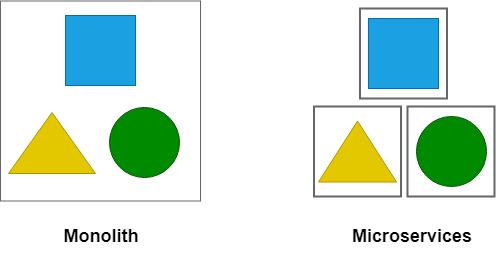
\includegraphics[scale=0.6]{img/monolith-vs-micro}
    \caption[Vergelijking tussen een monolith en microservices applicatie]{Vergelijking tussen een monolith en microservices applicatie \cite{SourceFuse2018}}
\end{figure}

Een microservice architectuur wordt steeds meer gebruikt in organisaties bij het ontwikkelen van hun applicaties. Dit vooral omwille van voordelen zoals simpliciteit en flexibiliteit. Een ander voordeel aan het implementeren van microservices is het gemak waarmee fouten kunnen opgespoord en behandeld worden. Wanneer een service fouten produceert, zal deze sneller te vinden zijn. Aangezien een enkele service vaak slechts een klein stuk software betreft, zal het probleem snel opgelost kunnen worden. Er is dus sprake van een verhoogd overzicht in de structuur van een applicatie. De schaalbaarheid en het onderhoudsgemak zijn nog twee belangrijke zaken om te vermelden. Er is ook een negatief aspect aan microservices verbonden, namelijk een enorm planning aspect bij de implementatie van deze structuur. Indien op een foute manier toegepast, kan het leiden tot een gedistribueerde monolithische structuur, wat het slechtste van de twee werelden combineert \autocite{Carey2018}. 

Logging is een enorm belangrijk aspect van een microservice architectuur. Om een applicatie met microservices te kunnen debuggen moet er een gecentraliseerd logging platform aanwezig zijn. Hoe groter de applicatie, hoe moeilijker om het overzicht van al deze services te bewaren. Elke service heeft een aparte console waarnaartoe gelogd wordt. Dit maakt het moeilijk om alles te doorzoeken in geval van bugs \autocite{SourceFuse2018}. 

Be-Mobile maakt gebruik van een microservice architectuur om hun producten te ontwikkelen. Elk verkeersevent dat binnenkomt, wordt van de ene microservice naar de andere doorgegeven en steeds verder verwerkt. Zo wordt een chain gecreëerd. Er zijn meerdere chains die doorlopen kunnen worden. Dit hangt af van het soort event dat heeft plaatsgevonden. Een belangrijk punt bij het implementeren van een gecentraliseerd logging platform voor Be-Mobile is dus het visualiseren van de chain die gevolgd werd door een bepaald event door middel van tracing \autocite{jens2019}.

\section{Kubernetes}
\label{sec:kubernetes}

\subsection{Wat is Kubernetes?}
De basis van Kubernetes is dat het een open-source systeem is voor het beheren van applicaties die in een container (zie 2.5 Docker) geplaatsd zijn. Containers zijn omhulsels voor services. Alles wat nodig is om de service te kunnen runnen, wordt voorzien door de container. Kubernetes draait als een samenhangende cluster (zie figuur 2.2) zodat men  componenten en services doorheen verschillende infrastructuren kan beheren. De manier waarop applicaties gehost worden hangt af van de manier waarop Kubernetes geconfigureerd is. Het is mogelijk om een applicatie te runnen als een DaemonSet, waardoor er in elke node een instantie van de applicatie gerund wordt. Ook zorgt deze configuratie er voor dat er automatisch een nieuwe instantie van de applicatie gecreëerd wordt bij het aanmaken van een nieuwe node. Dit is slechts een voorbeeld van de mogelijkheden van Kubernetes. De optimale configuraties van de onderzochte logging solutions komen later aan bod in TODO: REFEREER NAAR PROOF OF CONCEPT \autocite{ellingwood2018}.

\begin{figure}[ht]
    \centering
    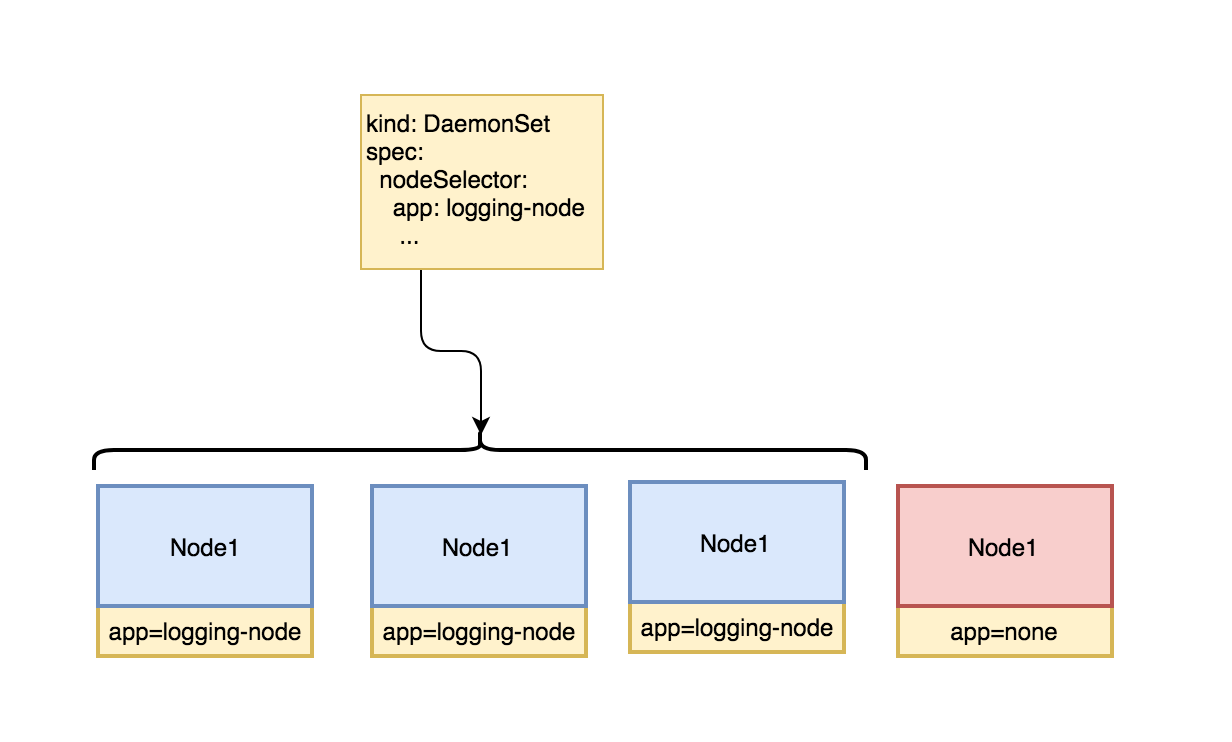
\includegraphics[scale=0.4]{img/kubernetes_daemonset}
    \caption[Kubernetes DaemonSet voorbeeld]{Kubernetes Daemonset voorbeeld \cite{techstories2017}}
\end{figure}

\subsection{Architectuur}
Kubernetes bestaat uit een master-minion architectuur (zie figuur 2.3) waar een master server het brein van de cluster voorstelt. Deze is een gateway om verschillende API's bloot te stellen aan de gebruikers. Verder is de master ook verantwoordelijk voor het controleren van de gezondheid van de cluster, scheduling van alle taken, en de communicatie tussen alle componenten \autocite{ellingwood2018}.

De `minions' worden nodes genoemd en zijn de servers waarop een of meerdere containers gerund worden. De nodes krijgen instucties van de master over wat er moet gebeuren met verschillende containers. Het creëren van nieuwe containers, het vernietigen van oude containers, en het forwarden van data zijn enkele van de taken van de nodes \autocite{ellingwood2018}.

Een node bestaat uit een of meerdere pods (zie figuur 2.3). Elke pod is een groep van een of meerdere containers die gedeployed zijn. Deze pods zijn er om nog verder onderscheid te kunnen maken in de configuratie. Elke pod heeft een eigen IP adres binnen de cluster en elke container in een pod deelt een IP adres, hostnaam, en andere zaken \autocite{learnitguide2018}.

Om een cluster op te starten wordt gebruik gemaakt van configuratie files in de vorm van YAML files. YAML staat voor `YAML Ain't Markup Language` en wordt gebruikt om configuratie mee te maken \autocite{grav}) Hierin wordt de gewenste structuur beschreven. De master server leest deze configuraties en delegeert de opdrachten aan zijn nodes om de gewenste structuur te bereiken \autocite{ellingwood2018}.

\begin{figure}[ht]
    \centering
   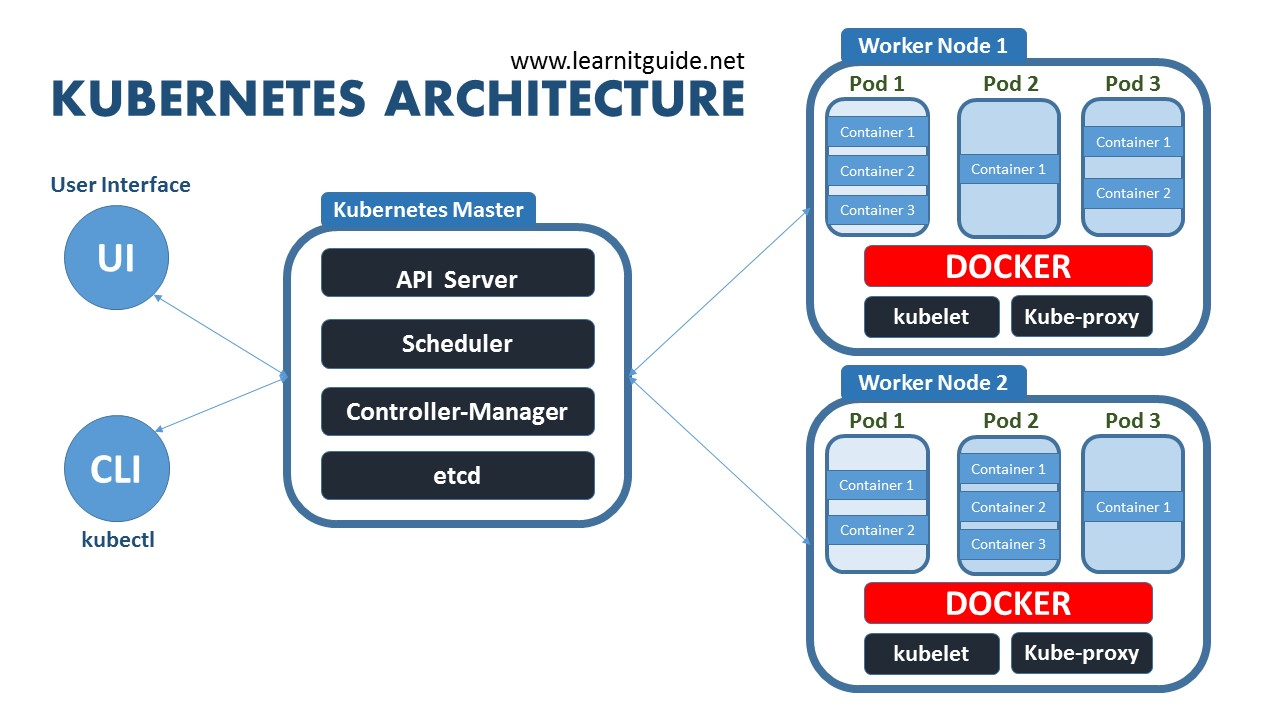
\includegraphics[scale=0.4]{img/kubernetes_architecture_explained}
    \caption[Kubernetes Architecture]{Kubernetes Architecture \cite{learnitguide2018}}
\end{figure}

\section{Docker}
\label{sec:docker}

\subsection{Situatie voor Docker}
Voor de komst van Docker was de manier waarop software uitgevoerd werd volledig anders. Software laat het niet steeds toe om uitgevoerd te worden in dezelfde omgeving als een ander soort software. Maar hoe slaagde men er in om toch alle programma's werkende te krijgen? Ze maakten gebruik van virtual machines. Deze lieten toe om verscheidene programma's simultaan uit te voeren op dezelfde hardware. Hoewel virtuele machines een oplossing boden voor het probleem, was de kost hoog. Virtuele machines zijn zware software die elk enkele gigabytes in grootte zijn.Verder bracht deze oplossing andere problemen met zich mee  zoals software updates, continuous delivery, en continuous integration \autocite{yegulalp2018}.

\subsection{De oplossing}
Docker containers zijn de oplossing voor dit probleem. Ze zijn licht, draagbaar, en flexibel. De manier waarop ze werken is simpel (zie figuur 2.4). Elk programma of stuk software wordt omhuld in een container die afzonderlijk draaiende wordt gehouden zoals een virtuele machine. Kortom wil dit zeggen dat alles geïsoleerd wordt en er dus geen problemen ontstaan met componenten die niet samen kunnen uitgevoerd worden. Zoals reeds besproken maakt Kubernetes uitstekend gebruik van containers. Het brengt deze met elkaar in contact of houdt ze net gescheiden. Zo kunnen containers die afhangen van elkaar, aan elkaar vastgehaakt worden in een pod. Een andere functionaliteit van Docker container is de herbruikbaarheid. Eens een container aangemaakt is kan deze via Kubernetes meerdere malen herbruikt worden of simultaan uitgevoerd worden \autocite{yegulalp2018}.

\begin{figure}[ht]
    \centering
    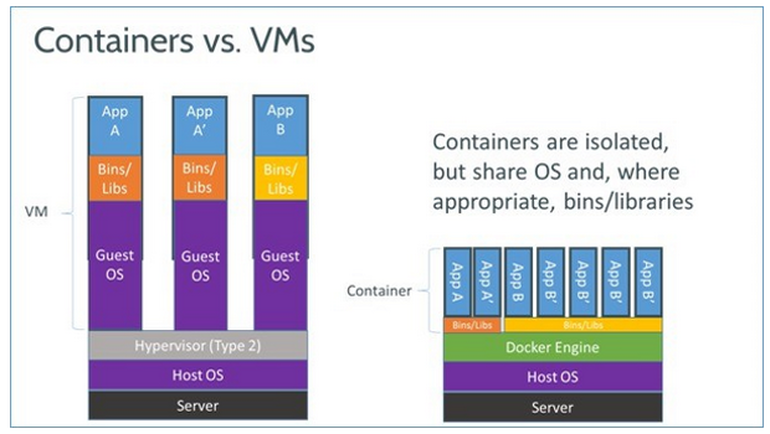
\includegraphics[scale=0.6]{img/docker-vm-vergelijking}
    \caption[Vergelijking tussen VM's en Docker containers]{Vergelijking tussen VM's en Docker containers \cite{vaughan2018}}
\end{figure}

\section{Logs, traces, en metrics}
\label{sec:log}

\subsection{Wat is een log?}

Een log is de documentatie van events die zich voordoen. De meeste systemen en softwareapplicaties bevatten automatische log generatie. De logs worden dan opgeslagen in een file waar ze bijgehouden worden om later geëvalueerd te worden. Men kan ook opteren om bij het schrijven van een eigen applicatie zelf logging te voorzien om de eigen applicatie beter te kunnen opvolgen en te debuggen. De keuze ligt bij de developer om deze logs dan op te slaan in een file. Standaard worden logs getoond in de console met een timestamp, bericht, en een log niveau \autocite{Techopedia}.

\subsection{Belang van logging}

Logging is een belangrijk aspect van software development. Maar wat is nu het belang van logging? De tijd die een developper investeert in het correct loggen van de belangrijke informatie in een applicatie is hopelijk toch geen verspilde tijd? 

Ten eerste is er het belang van duidelijkheid in een applicatie. Logs zorgen er voor dat er precies kan gezien worden wat er gaande is in een applicatie. Bij het debuggen zijn logs van onschatbare waarde om na te gaan wat er fout is gegaan \autocite{logdna2018}.

Ten tweede hebben logs belang voor het hele bedrijf. Wanneer er sprake is van een bedrijf met verschillende teams die elk verantwoordelijk zijn voor hun eigen deel van een applicatie, zullen er restricties te vinden zijn in de rechten van elk team. Een developper hoort geen rechten te hebben op repositories waar hij zelf niet mee in contact komt. Bij het debuggen van een probleem kan een developper de logs van software waar hij zelf geen rechten op heeft toch bekijken. Zonder logs zouden er rechten toegekend moeten worden om de code te bekijken op zoek naar het probleem \autocite{czanik2013}.

\subsection{Golang logging frameworks}

Bij Be-Mobile wordt Golang gebruikt om de backend van hun microservices op te bouwen. Deze relatief nieuwe taal heeft reeds enkele ondersteunde opties op vlak van logging frameworks. De twee meest gebruikte zijn Glog en Logrus \autocite{Dietrich2018}. In dit onderzoek zal enkel Logrus ter sprake komen omdat deze het meest actief ondersteund wordt en omdat Logrus het gekozen logging framework is van Be-Mobile \autocite{jens2019}.

Glog:
\begin{itemize}
    \item Uitgebracht door Google;
    \item Simpele stijl, gebaseerd op die van Golang zelf \autocite{Dietrich2018};
    \item Laatste commit 25 januari 2016 \autocite{Glog2013};
\end{itemize}

Logrus:
\begin{itemize}
    \item Community driven;
    \item Goede ondersteuning;
    \item Laatste commit 3 maart 2019 \autocite{sirupsen2014};
\end{itemize}

\subsection{Logrus}
“Logrus is een gestructureerde logger voor Go, volledig API compatibel met de standaard library logger” (sirupsen, s.d.). Logrus is een uitbreiding op de standaard library logger. Het biedt een wijd gamma aan functionaliteit bij het loggen van events. De verschillende levels waarin gelogd kan worden zijn: Trace, Debug, Info, Warning, Error, Panic, en Fatal. Deze levels zorgen voor een duidelijke weergave van het gelogde event. Hiermee kan de gebruiker, indien deze gebruik maakt van een log collector, filteren op level en zo vlotter de verschillende events doorlopen tijdens het debuggen. Verder kunnen ook nog andere fields toegevoegd worden die de gebruiker extra mogelijkheden biedt tijdens het filteren. Ten slotte kunnen de logs zowel de console als een wijd gamma andere keuzes als output gebruiken. Logrus kan gebruik maken van hooks om de data door te sturen naar message brokers zoals redis en kafka, alsook naar een file die lokaal opgeslagen kan worden. Hooks zijn zoals de term al doet vermoeden inhakingen op logrus. Hiermee kan er vooraleer de logs in de output verschijnen nog iets met gedaan worden \autocite{sirupsen2014}.

\subsection{Tracing}

Naast logs is er nog een tweede soort data die belangrijk is in microservices, trace data. De bedoeling van dit soort data is het achterhalen van de volledige chain die doorlopen wordt door een enkel event. Doorheen de chain kan dan gekeken worden hoelang elke microservice gewerkt heeft of hoelang een bepaalde API-call heeft geduurd (zie figuur 2.5). Deze data kan daarna gebruikt worden om metrics mee te maken, bv. De gemiddelde duur van een API-call. Zo kunnen uitschieters onderzocht worden om tot de kern van een probleem te komen \autocite{Rouse2018}.

OpenTracing is een specificatie welke gebruikt wordt door de grootste Tracers. Omdat OpenTracing vendor-neutral is kan men dus kiezen welke Tracer men uiteindelijk wil gebruiken bij het verzamelen van traces (Rouse, 2018). De meest gebruikte Tracers voor Go zijn Zipkin en Jaeger \autocite{Sabic2018}.

\begin{figure}[ht]
    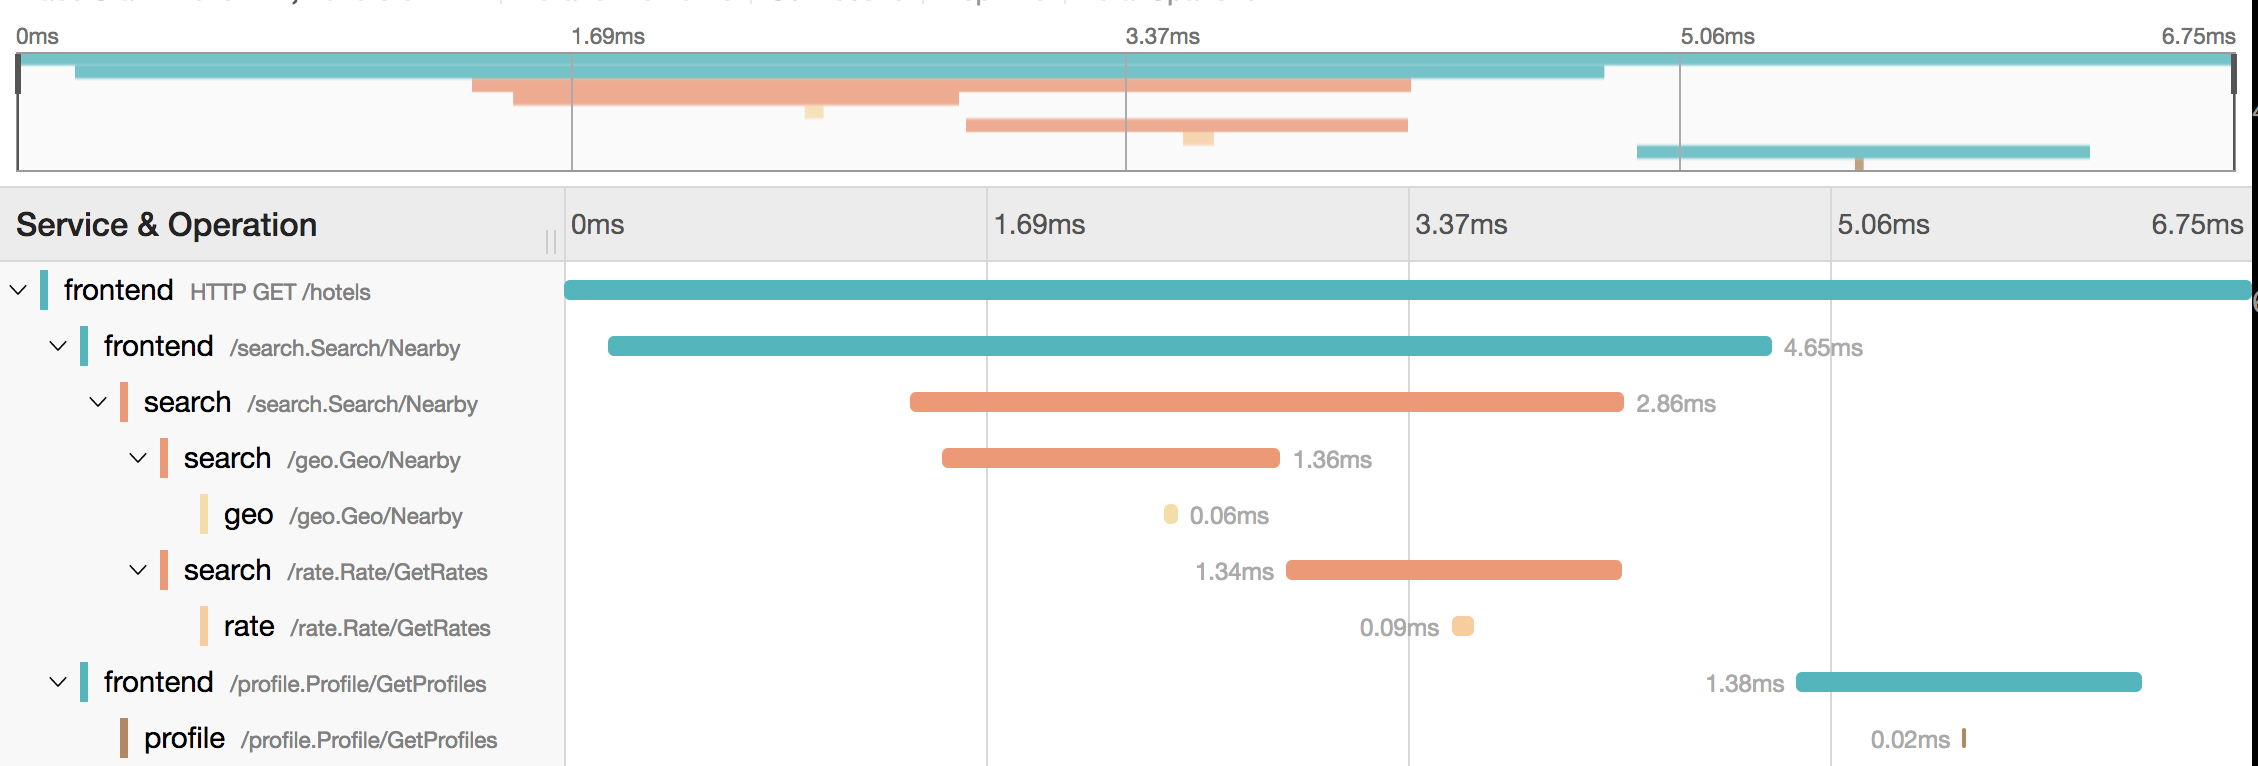
\includegraphics[scale=0.4]{img/tracing_voorbeeld}
    \caption[Voorbeeld van tracing in Jaeger]{Voorbeeld van tracing in Jaeger \cite{harlow2015}}
\end{figure}

\subsection{Metrics}

De derde en laatste soort data die gebruikt wordt om een applicatie te monitoren is metrics. Deze houden de systeembeheerders op de hoogte van de status van de applicatie. Dit werk maakt een vergelijkende studie tussen de meest populaire logging solutions, dus buiten deze korte introductie zal er niet verder ingegaan worden op metrics. Metrics maken het mogelijk om in een oogopslag de algemene gezondheid van een applicatie te zien (zie figuur 2.6). Er wordt gebruik gemaakt van grafieken en statistieken om dit weer te geven. Het verschil met tracing is dat metrics de volledige situatie van een applicatie omvatten en tracing een detail observatie is van bepaalde events of services in de applicatie \autocite{reichert2018}.
\\
\begin{figure}[ht]
    \centering
    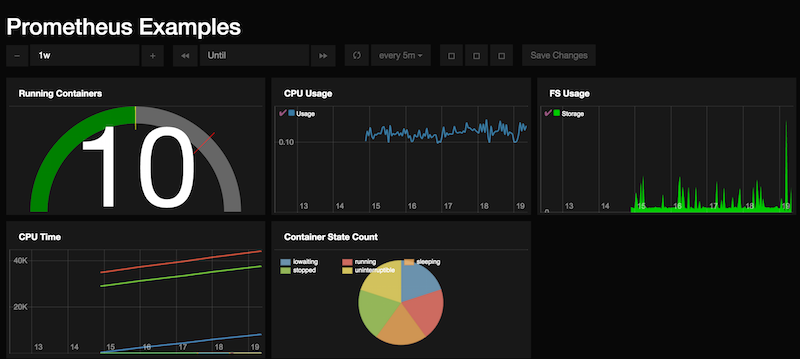
\includegraphics[scale=0.8]{img/prometheus_example}
    \caption[Voorbeeld van metrics in Prometheus]{Voorbeeld van metrics in Prometheus \cite{christner2015}}
\end{figure}

\section{Logging solutions}
\label{sec:logging-solutions}

\subsection{Wat is een logging solution en hoe werkt het?}
Voor er meer in detail gegaan wordt over de logging solutions die getest werden in dit werk, zal er een definitie beschreven worden wat beschouwd wordt als een logging solution.
Een logging solution is een tool of een combinatie van tools die toelaat om efficiënt aan log management te doen. Het hele proces van logging doorloopt verschillende stappen (figuur 2.7) \autocite{logdna2018}.

\begin{figure}[ht]
    \centering
    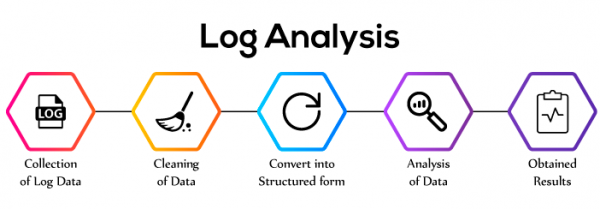
\includegraphics[scale=0.6]{img/log_proces}
    \caption[Het logging proces]{Het logging proces \cite{nastel}}
\end{figure}

\begin{enumerate}
    \item Data collectie: Ingestion en log aggregation. Een eerste stap hierbij is data die verzameld wordt vanuit verschillende bronnen. Deze bronnen kunnen de console logs zijn, de opgeslagen log files, syslog, etc. De verantwoordelijk voor dit proces is een collector. De tweede stap is het correct formateren van de verzamelde logs. Zonder deze stap zou de data niet uniform genoeg zijn om in een latere fase de analyse hierop uit te voeren \autocite{logdna2018}. 
    \item Filtering en analyse: De volgende schakel in het verhaal is de analyse. Eens de logs allemaal hetzelfde formaat hebben, kan er gefilterd worden. Dit kan op verschillende manieren gebeuren. Er kan gefilterd worden op tijd, log level (zie 2.6.4 Logrus), extra toegevoegde tags, service waar de log plaatsvond, en nog veel meer. De analyse gebeurt op basis van grafieken en statistieken. Er is mogelijkheid om bepaalde statistieken bij te houden om gemakkelijk het overzicht te bewaren over situaties die zich kunnen voordoen  \autocite{logdna2018}.
    \item Reporting. Nadat de analyse afgerond is en alle grafieken en statistieken aangemaakt zijn, kan er reporting ingesteld worden voor deze. Er kunnen alarmen aangemaakt worden die op verschillende manieren de verantwoordelijke personen op de hoogte stellen dat een bepaalde situatie zich heeft voorgedaan. Bijvoorbeeld wanneer een service een bovengemiddeld aantal error logs produceert op korte termijn  \autocite{logdna2018}.
    \item Opslag. Hierbij worden logs opgeslagen voor een bepaalde duur zodat deze beschikbaar blijven  \autocite{logdna2018}.
\end{enumerate}

\subsection{Belangrijke punten in een logging solution}

Wat is er belangrijk bij het zoeken naar een logging solution? Waar moet rekening mee gehouden worden in een beslissing?

\begin{enumerate}
    \item  Schaalbaarheid is van enorm belang in de groeiende sector van IT. Een bedrijf dat snel groeit kan zich niet veroorloven steeds opnieuw de hele structuur aan te passen om deze te laten meegroeien. Een goede logging solution kan automatisch of met zo weinig mogelijk werk meegroeien met het bedrijf \autocite{logdna2018}. Een voorbeeld hierin is Be-Mobile (zie 2.1 Be-Mobile) \autocite{jens2019}. 
    \item Overhead. Dit is de impact van de gekozen oplossing op het systeem. Zware oplossingen kunnen de applicatie vertraging en minder performant maken \autocite{gifford2015}.
    \item Installatie \autocite{logdna2018}.
    \item Gebruiksgemak. Alle developpers in het bedrijf moeten dezelfde tool kunnen gebruiken \autocite{logdna2018}.
    \item Snelheid waarmee logs getoond kunnen worden in de gekozen visualisatie tool \autocite{logdna2018}.
    \item Automatische parsing van de logs bij het innemen van de logs \autocite{logdna2018}.
\end{enumerate}

\subsection{ELK}
ELK is een acronym voor Elasticsearch, Logstash, Kibana. Dit zijn de drie componenten die een ELK stack bevat. Vaak wordt bovenop deze componenten ook gebruik gemaakt van Beats. Dit is een lichtgewicht data collector die handig kan zijn bij Kubernetes deployments met vele nodes. Bij complexe pipelines zoals Be-Mobile waar een hoge throughput aan data aanwezig is, wordt aangeraden om gebruik te maken van een message broker tussen de data collectie en data processing die voor een betrouwbare volgorde zorgt. Voorbeelden hiervan zijn Kafka, RabbitMQ, Redis (zie figuur 2.8) \autocite{berman2018-12}. 

\begin{figure}[ht]
    \centering
    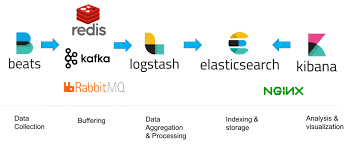
\includegraphics[scale=1]{img/elk-proces}
    \caption[Volledige ELK stack]{Volledige ELK stack \cite{berman2018-12}}
\end{figure}

De werking van ELK gaat als volgt. Logs worden geproduceerd en opgeslagen in files. Beats verzamelt deze en stuurt ze meteen door naar een message broker. Daarna volgt Logstash. Deze haalt de logs op van de message broker en verwerkt deze. De logs worden hier gefilterd. Er kunnen via grok nieuwe benamingen gegeven worden aan delen van de log lijn. Ook kunnen dingen zoals datum, IP-adres, en dergelijke toegevoegd worden. Uiteindelijk worden de logs doorgestuurd naar Elasticsearch waar ze opgeslagen worden. De werking van Logstash wordt volledig bepaald door een config file. De laatste stap is Kibana, dit is de visualitie tool. Kibana gebruikt Elasticsearch als data source om de logs op te halen en toont deze met extra kleur accenten op tags om duidelijkheid te creëren \cite{levy2015,berman2018-12}. 

De ELK stack is een goede logging oplossing omdat het een enorm krachtige tool is in combinatie met een gemakkelijk installatie. Naast zijn vele voordelen zijn er ook wat mindere punten aan de ELK stack die genoemd moeten worden. Hoewel de basis installatie vrij simpel uit te voeren is, wordt deze al snel ingewikkelder naargelang de grootte van de cluster waarop deze geïnstalleerd wordt. Er zijn veel factoren waar rekening gehouden mee moet worden en een verkeerde implementatie kan leiden tot inefficiëntie of zelfs crashes op lange termijn. Om deze reden hoort er genoeg aandacht besteed te worden aan resource management bij het opzetten van de ELK stack \autocite{gifford2016}.

\subsection{EFK}

\begin{figure}[ht]
    \centering
    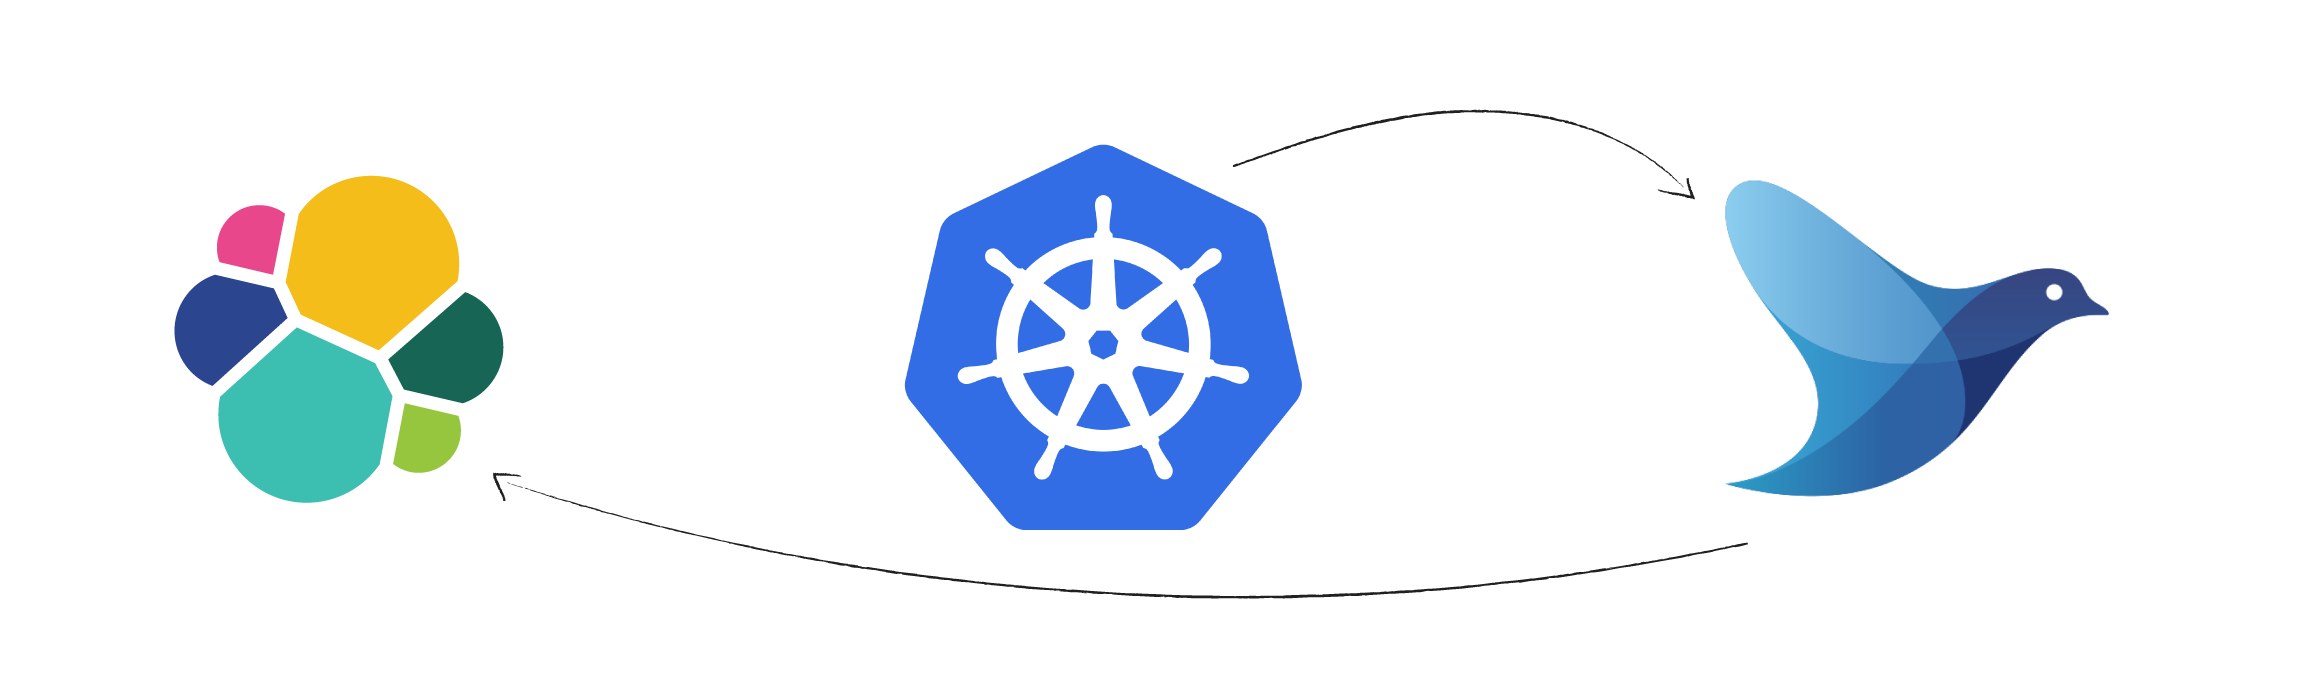
\includegraphics[scale=0.15 ]{img/EFK_logo}
    \caption[EFK stack]{EFK stack \cite{petrausch}}
\end{figure}

Soortgelijk aan ELK, is EFK een acronym voor Elasticsearch, Fluentd, Kibana (zie figuur 2.9). Hierbij wordt op een soortgelijke manier gewerkt als bij ELK maar wordt Logstash vervangen door Fluentd. De redenen hiervoor zullen hieronder verder uitgelegd worden. Wanneer gewerkt wordt met Kubernetes moet de afweging gemaakt worden tussen gebruik van Fluentd en Fluentbit. Deze laatste is een nieuwere, kleinere variant van de eerste. Qua functionaliteit zijn ze beiden bijna evenwaardig met als enige grote verschil het aantal ondersteunde plugins wat veel hoger is bij Fluentd. De grote kracht van Fluentbit is dan weer de grootte ervan. Met slechts 450KB is de voetafdruk van Fluentbit op gedistribueerde omgevingen enorm klein in vergelijking met Fluentd. Fluentbit is dan ook ontwikkeld met gedistribueerde omgevingen als primaire use case \autocite{berman2018-06}.

Deze verschillen tussen Logstash en Fluentd zijn als volgt:
\begin{enumerate}
    \item Taal. Logstash is geschreven in JRuby welke een Java implementatie is van Ruby en dus een Java Runtime vereist. Fluentd daarentegen is geschreven in CRuby, een C implementatie van Ruby en heeft dus minder vereisten qua omgeving \autocite{harikumar2018}.
    \item De routing van events. Waar Logstash voor routing zorgt door gebruik te maken van if-then statements, gebruikt Fluentd tags om hetzelfde te doen. Fluentd lijkt daarop iets makkelijk om te configureren \autocite{harikumar2018}.
    \item Plugins. Zoals eerder vermeld heeft Fluentd een enorm grote hoeveelheid plugins met meer dan 350 plugins voor input, output, of verwerking van data. Logstash beschikt ook over een aantal plugins. Het grote verschil zit in de plaats waar deze plugins te vinden zijn. In tegenstelling tot Fluentd is er bij Logstash wel een gecentraliseerde github repository waar alle plugins te vinden zijn \autocite{harikumar2018}.
    \item Message queue. Door gebruik te maken van Fluentd of Fluentbit wordt de nood aan een message broker geëlimineerd. Fluentd heeft namelijk een ingebouwde message queue die alle inkomende messages zelf correct verwerkt. Hierdoor kan Fluentd, in tegenstelling tot Logstash, geïmplementeerd worden in complexe systemen zonder externe message broker \autocite{harikumar2018}. 
\end{enumerate}

Om optimaal gebruik te maken van de EFK stack in een gedistribueerde omgeving op een Kubernetes cluster moet gebruik gemaakt worden van zowel Fluentbit als Fluentd. In deze setup bevat elke node in de cluster een Fluentbit instantie die de logs van die node verzameld en doorstuurt naar de algemene Fluentd instantie op de cluster. Deze fungeert als aggregator en verwerkt de logs om ze daarna door te sturen naar de gekozen output \autocite{berman2018-06}.

\subsection{Graylog}
Graylog is ontstaan in 2009 in een tijd waar logging oplossingen, laat staan open source logging oplossingen quasi onbestaand waren. De marktleider in die tijd had een kostelijke licentie en daarom ontwikkelde de oprichter van Graylog een eigen open source oplossing. Dit wil zeggen dat Graylog vanaf het begin al een logging oplossing hoorde te zijn. Dit in tegenstelling tot ELK op basis van Elasticsearch, welke een full text search engine is. Graylog maakt zelf ook nog steeds gebruik van Elasticsearch als opslagplaats maar de Graylog server die voor de databank zit wordt het gebruik ervan geoptimaliseerd voor logs \autocite{graylog}.

De ouderdom van de Graylog betekent dat deze niet is geoptimaliseerd voor het gebruik ervan in een gedistribueerde omgeving zoals een Kubernetes cluster. Er is wel reeds documentatie toegevoegd om Graylog werkende te krijgen op een Kubernetes cluster \autocite{lumiq2017}.  

\subsection{Grafana Loki}
De meest recente logging solution, nog steeds in alfa ontwikkeling maar wel reeds beschikbaar. Wat meteen duidelijk wordt, is dat Loki ontwikkeld is voor het gebruik in grote, complexe, gedistribueerde omgevingen. Het is ontwikkeld om zoveel mogelijk logs te kunnen opslaan voor zo weinig mogelijk geld. Tot hiertoe zijn alle databanken gebaseerd op volledige indexering bij het opslaan van logs, dit zorgt voor heel wat opslagruimte die noodzakelijk is om alles draaiende te houden. Loki stapt af van indexering en is gebaseerd op Prometheus, een ander product van Grafana dat gebruikt wordt voor de opslag van metrics. De manier waarop Loki logs opslaat, werkt op basis van labels en enkel de metadata wordt geïndexeerd \autocite{oleksii2019}.

\begin{figure}[ht]
    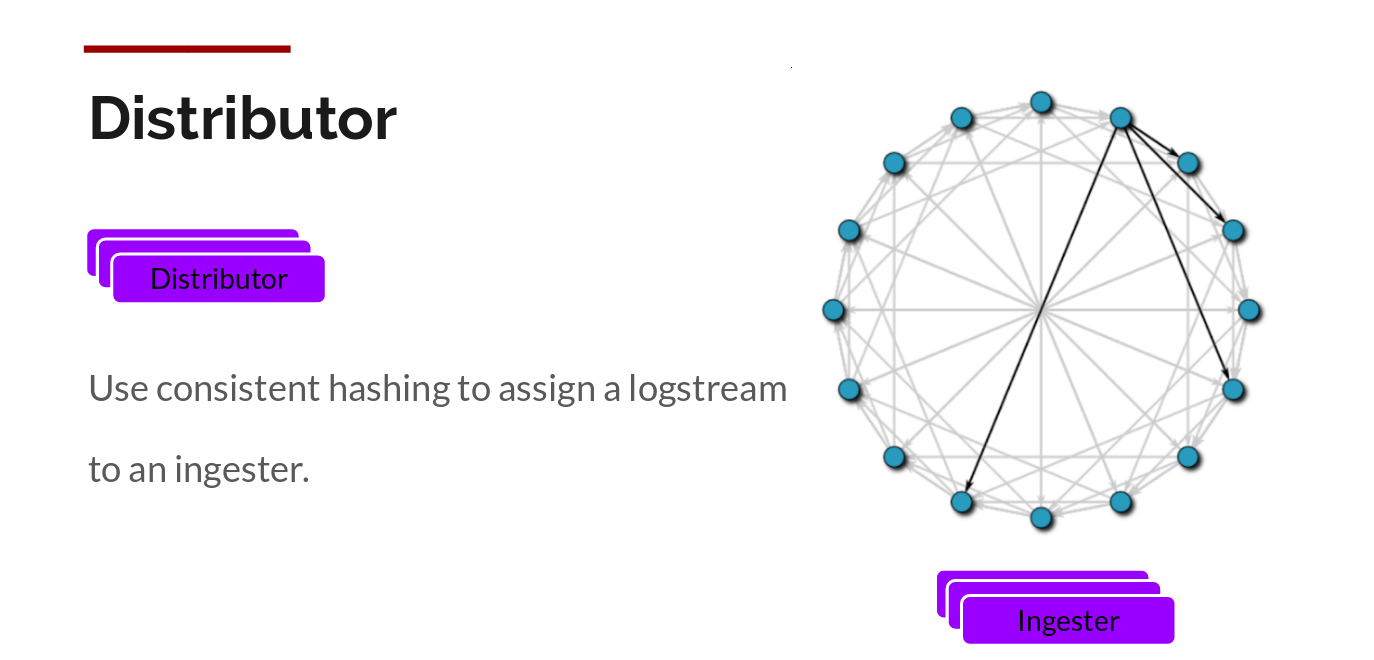
\includegraphics[scale=0.3]{img/loki_distributor}
    \caption[Grafana Loki distributor]{Grafana Loki distributor \cite{loki}}
\end{figure}

\begin{figure}[ht]
    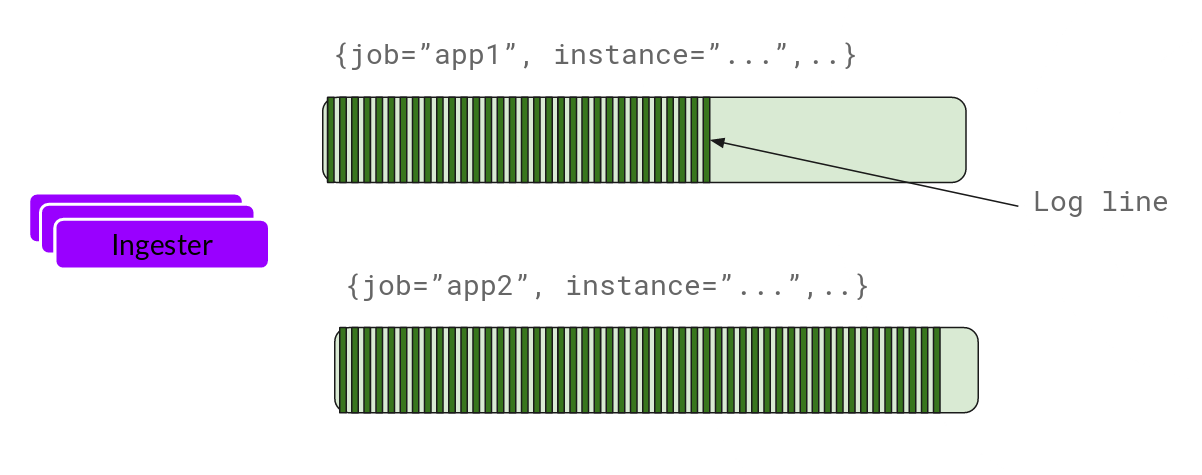
\includegraphics[scale=0.3]{img/loki_ingester}
    \caption[Grafana Loki Ingester]{Grafana Loki Ingester \cite{loki}}
\end{figure}

Een loki 'stack' bestaat uit 3 belangrijke componenten:
\begin{enumerate}
   \item Promtail is verantwoordelijk voor het verzamelen van logs. Het is een scraper die op zoek gaat in alle Kubernetes pods naar log files en deze daarna doorstuurt naar Loki. Promtail wordt geïnitialiseerd op basis van een config file waarin beschreven wordt welke log files doorgestuurd worden, welke genegeerd worden, en welke anders genoemd worden. Soortgelijk aan Fluentbit zal Promtail ook in elke node aanwezig zijn en logs doorsturen naar een algemene loki instantie \autocite{veeramachaneni2018}.
   \item Loki is de datasource van de stack. Het maakt gebruikt van een distributor (zie figuur 2.10) om logs te verspreiden over verschillende ingesters (zie figuur 2.11) vooraleer de logs in een databank terecht komen. De manier waarop Loki logs opslaat is ook anders dan de concurrentie. De ingesters verzamelen soortgelijke logs in chunks. Wanneer een chunck opgevuld is, wordt deze opgeslagen in een Object Storage. Default is dit een lokale Object Storage. De indexen van deze logs worden daarna in een NoSQL database opgeslagen om snel opgehaald te kunnen worden. Deze manier van opslag zorgt voor een snelle ophaling van logs wanneer deze opgevraagd worden in Grafana. Ook zorgt deze manier van opslag voor een grote schaalbaarheid \autocite{veeramachaneni2018}.
   \item Grafana is de frontend die zowel Loki als Prometheus en andere bronnen kan gebruiken als data source. Hier worden de logs gevisualiseerd. Op moment van schrijven van dit werk is er enkel tekstuele filtreerbaarheid beschikbaar op basis van een eigen query taal van Grafana. Ook deze is nog onder constructie en verwacht binnenkort een upgrade. Nummers worden dan ook filtreerbaar met mogelijkheid tot filteren op datum of bepaalde getallen vergelijken \autocite{githubLoki2019, veeramachaneni2018}. 
\end{enumerate}

%%=============================================================================
%% Methodologie
%%=============================================================================

\chapter{Methodologie}
\label{ch:methodologie}

%% TODO: Hoe ben je te werk gegaan? Verdeel je onderzoek in grote fasen, en
%% licht in elke fase toe welke stappen je gevolgd hebt. Verantwoord waarom je
%% op deze manier te werk gegaan bent. Je moet kunnen aantonen dat je de best
%% mogelijke manier toegepast hebt om een antwoord te vinden op de
%% onderzoeksvraag.

Na de onderzoeksfase van dit werk in de vorm van een literatuurstudie (zie Hoofdstuk~\ref{ch:stand-van-zaken}) volgt hieronder een requirementsanalyse die een opsomming maakt van de belangrijkste requirements. Deze zullen later in de conclusie (zie Hoofdstuk~\ref{ch:conclusie}) belangrijk zijn in het beoordelen van de meest geschikte oplossing in deze situatie. Wegens het gebrek aan open-source oplossingen zal dit werk slechts 4 oplossingen vergelijken namelijk: ELK, EFK, Graylog, en Loki. Dit zorgt ervoor dat een long en short list niet nodig zijn in dit onderzoek en deze zullen dus achterwege gelaten worden. 

De uitwerking van een testomgeving zal als volgt gebeuren. Wegens de manier waarop de mensen achter Kubernetes Minikube hebben opgebouwd, is het niet mogelijk om meerdere nodes te installeren op een eigen Minikube. Bijgevolg is het dus niet mogelijk om een testomgeving op te zetten waarbij gebruik gemaakt wordt van meerdere nodes. Dit zorgt ervoor dat de complexiteit van de Kubernetes testomgeving drastisch daalt en vervangen kan worden door een lokale testomgeving. Hierbij zullen 2 Go services elk in hun eigen Docker container draaiende gehouden worden terwijl elk van de logging oplossingen getest zullen worden. De services bestaan uit een oneindige loop die steeds enkele logs per second zal produceren. Deze logs worden daarna opgeslagen in een logfile. Deze logfile wordt vervolgens gelezen door de log collector en doorgestuurd naar een opslagplaats. Als laatste worden de logs opgehaald uit de databank door een frontend die deze visualiseert voor de gebruiker.

\textbf{\underline{Go Services}}\\
\begin{lstlisting}[caption=Log generator main function]
import (
    "errors"
    "os"
    "time"
    
    "github.com/sirupsen/logrus"
)

func main() {
    w, err := os.Create("/Users/benjaminvaniseghem/Documents/logs/logfile1.log")
    if err != nil {
        panic(err)
    }
    logger := logrus.New()
    logger.SetOutput(w)
    for {
        logger.Info("Info message")
        logger.Warn("Warning message")
        logger.Error("Error message", errors.New("Error"))
        time.Sleep(1200 * time.Millisecond)
    }
}
\end{lstlisting}

\begin{lstlisting}[caption=Log generator 2 main function ]
import (
    "errors"
    "os"
    "time"
    
    "github.com/sirupsen/logrus"
)

func main() {
    w, err := os.Create("/Users/benjaminvaniseghem/Documents/logs/logfile2.log")
    if err != nil {
        panic(err)
    }
    logger := logrus.New()
    logger.SetOutput(w)
    for {
        logger.Info("Info 2 message")
        logger.Warn("Warning 2 message")
        logger.Error("Error message 2", errors.New("Error"))
        time.Sleep(1200 * time.Millisecond)
    }
}
\end{lstlisting}

Nadat deze testomgeving klaar is, zullen een voor een de gekozen logging oplossingen hierin getest worden. Hieronder wordt het hele testproces besproken.
\begin{enumerate}
    \item Als eerste gebeurt de installatie en het correct configureren van de benodigde software van de oplossing. 
    \item Na de installatie zal gekeken worden naar de visualisatie van de logs. Hierbij wordt rekening gehouden met de mogelijkheden omtrent het implementeren van grafieken over de gegenereerde logs en alerting in bepaalde situaties.
    \item De volgende stap is het ophalen van specifieke logs. Dit kan in veel gevallen door middel van een query taal of bepaalde filters te gebruiken.
    \item Tot slot zal de installatie van de oplossing verwijderd worden zodat het proces zich kan herhalen met een andere oplossing.
\end{enumerate}

Om de testen te herhalen op een Kubernetes cluster zijn extra configuraties nodig. In het kader van dit onderzoek is het interessant om deze te bespreken. De extra configuraties van elke oplossing zullen besproken worden in hun eigen respectievelijke hoofdstuk.

\textbf{\underline{Kubernetes config file}}\\
Een Kubernetes config file bestaat uit veel parameters waardoor een service op veel manieren gedeployed kan worden. Hieronder zijn de belangrijkste algemene parameters opgesomd. In elk hoofdstuk van de logging oplossingen zullen de gebruikte parameters dieper uitgelegd worden.
\begin{itemize}
    \item apiVersion : Versie van de Kubernetes API dat gebruikt wordt
    \item kind: Welk soort object gecreëerd moet worden. Een object kan een van de volgende zijn: \begin{itemize}
        \item Pod
        \item Service
        \item Volume
        \item Namespace
        \item ReplicaSet
        \item Deployment
        \item StatefulSet
        \item DaemonSet
        \item Job
    \end{itemize}
    \item metadata: Extra informatie over het object om het makkelijker uniek te identificeren.
    \item spec: Hier bevindt zich de specificaties omtrent het object. Dit is veranderlijk voor elk soort object.
\end{itemize}

\section{Requirementsanalyse}
\begin{itemize}
    \item \textbf{Functionele requirements}
        \begin{itemize}
             \item Moet kunnen scalen naargelang de groeiende Kubernetes cluster
            \item Ondersteuning voor verschillende plugins die data extra kunnen verwerken of naar meerdere locaties kunnen doorsturen
            \item Moet logs efficiënt opslaan en ophalen
            \item Ondersteuning voor cluster omgevingen zoals Kubernetes
            \item Ondersteuning voor alerts
            \item Ondersteuning voor visualisatie zoals grafieken
        \end{itemize}
    \item \textbf{Niet-functionele requirements}
        \begin{itemize}
           \item Moet open source zijn
           \item Moet (relatief) eenvoudig te configureren zijn
           \item Moet (relatief) eenvoudig te gebruiken zijn
           \item Moet goed gedocumenteerd zijn
           \item Moet een zo klein mogelijke impact hebben op de servers
           \item Moet de logs overzichtelijk kunnen tonen
        \end{itemize}
\end{itemize}

Bovenstaande requirements kunnen als volgt ingedeeld worden met de MoSCoW-techniek \autocite{consortium}. Deze verdeeld de requirements in `Must have`, `Should have`, en `Could have` requirements. Deze verdelingen betekenen respectievelijk dat de requirement verplicht is, aanwezig zou moeten zijn maar niet doorslaggevend, of optioneel is.  

\begin{itemize}
    \item \textbf{Must have}
    \begin{itemize}
        \item Moet open source zijn
        \item Ondersteuning voor cluster omgevingen zoals Kubernetes
        \item Moet een zo klein mogelijke impact hebben op de servers
        \item Moet kunnen scalen naargelang de groeiende Kubernetes cluster
    \end{itemize}
    \item \textbf{Should have}
    \begin{itemize}
        \item Moet (relatief) eenvoudig te configureren zijn
        \item Moet (relatief) eenvoudig te gebruiken zijn
        \item Moet goed gedocumenteerd zijn
        \item Moet de logs overzichtelijk kunnen tonen
        \item Ondersteuning voor verschillende plugins die data extra kunnen verwerken of naar meerdere locaties kan doorsturen
         \item Ondersteuning voor visualisatie zoals grafieken
    \end{itemize}
    \item \textbf{Could have}
    \begin{itemize}
       \item Ondersteuning voor alerts
    \end{itemize}
\end{itemize}

Het hele test proces zal gebruik maken van een lokale testomgeving en zal dus niet het formaat hebben van een cluster zoals bij Be-Mobile of andere bedrijven die tot de doelgroep van dit onderzoek behoren. Bijgevolg zullen de requirements `Moet een zo klein mogelijke impact hebben op de servers`, `Moet kunnen scalen naargelang de groeiende Kubernetes cluster`, en `Ondersteuning voor cluster omgevingen zoals Kubernetes` niet op deze manier onderzocht kunnen worden. Voor de conclusie van deze requirements zal er gerefereerd worden naar documentatie over de oplossingen in kwestie. Deze gegevens zullen dan vergeleken worden met elkaar. 

Om het vergelijken van de oplossingen simpeler voor te stellen zal er voor elke requirement een cijfer van 1 tot 5 gegeven worden aan de oplossing in kwestie. Deze kunnen later vergeleken worden om een conclusie te vormen. Verder zal er een antwoord gegeven worden op de onderzoeksvraag. Zowel de conclusie als het antwoord op de onderzoeksvraag zijn te vinden in Hoofdstuk~\ref{ch:conclusie}













%%=============================================================================
%% ELK
%%=============================================================================

\chapter{ELK}
\label{ch:ELK}

\section{Installatie en configuratie}
Zoals reeds besproken in Hoofdstuk~\ref{subsec:ELK} ELK, bestaat deze stack uit drie belangrijke elementen die aangevuld kunnen worden met meerdere componenten om deze oplossing efficiënter te maken.
\begin{itemize}
    \item Logstash
    \item Elasticsearch
    \item Kibana
    \item Filebeat (optioneel, vooral in Kubernetes omgevingen)
    \item Message broker zoals Kafka, Redis,... (optioneel, vooral in Kubernetes omgevingen)
\end{itemize}

Logstash is opgebouwd vanuit een pull model. Dit wil zeggen dat Logstash op zoek gaat naar een gedefinieerde input bron waar logs te vinden zijn. Er zijn verschillende inputmogelijkheden zoals file en syslog. Logstash kan ook gebruikt worden met een pushmodel. Het stelt zichzelf open om logs te ontvangen van Filebeats om deze verder te verwerken en door te sturen naar Elasticsearch. Om deze demonstratie eenvoudig voor te stellen wordt gebruik gemaakt van een log generator plugin van Elastic. Deze plugin configuratie is te zien in Listing 4.1. Zo kan gefocust worden op de drie belangrijkste componenten.

\subsection{Lokale omgeving}

De eenvoudigste manier om een snelle testomgeving op te stellen is door gebruik te maken van een github repositoy met reeds bestaande configuratie en deze naar eigen wens aan te passen. Met de repository https://github.com/deviantony/docker-elk kan mits enkele aanpassingen een ELK stack uitgerold worden. Hierbij moet de input van de Logstash config in de pipeline folder nog aangepast worden naar de log generator die te zien is in Listing 4.1. Verder wordt gebruik gemaakt van een docker-compose.yaml file om alle services met één commando uit te rollen. Door het gebruik van authenticatie bij deze installatie moet ingelogd worden bij Kibana om verder te gaan. De inloggegevens zijn ook te vinden in de repository. 

Eens de setup uitgerold is moet er een index gecreëerd worden in Kibana om de logs te kunnen filteren. Daarna zijn de logs te zien in de `Discover` pagina zoals te zien is in Figure 4.1.


\begin{lstlisting}[caption=Log generator plugin config Logstash]
input {
    generator {
        lines => [
            "Dit is een test log",
            "Tweede test log",
            "Nog een test log"
        ]
        # Emit all lines 25 times.
        count => 25
    }
}
\end{lstlisting}

\begin{figure}[ht]
    \centering
    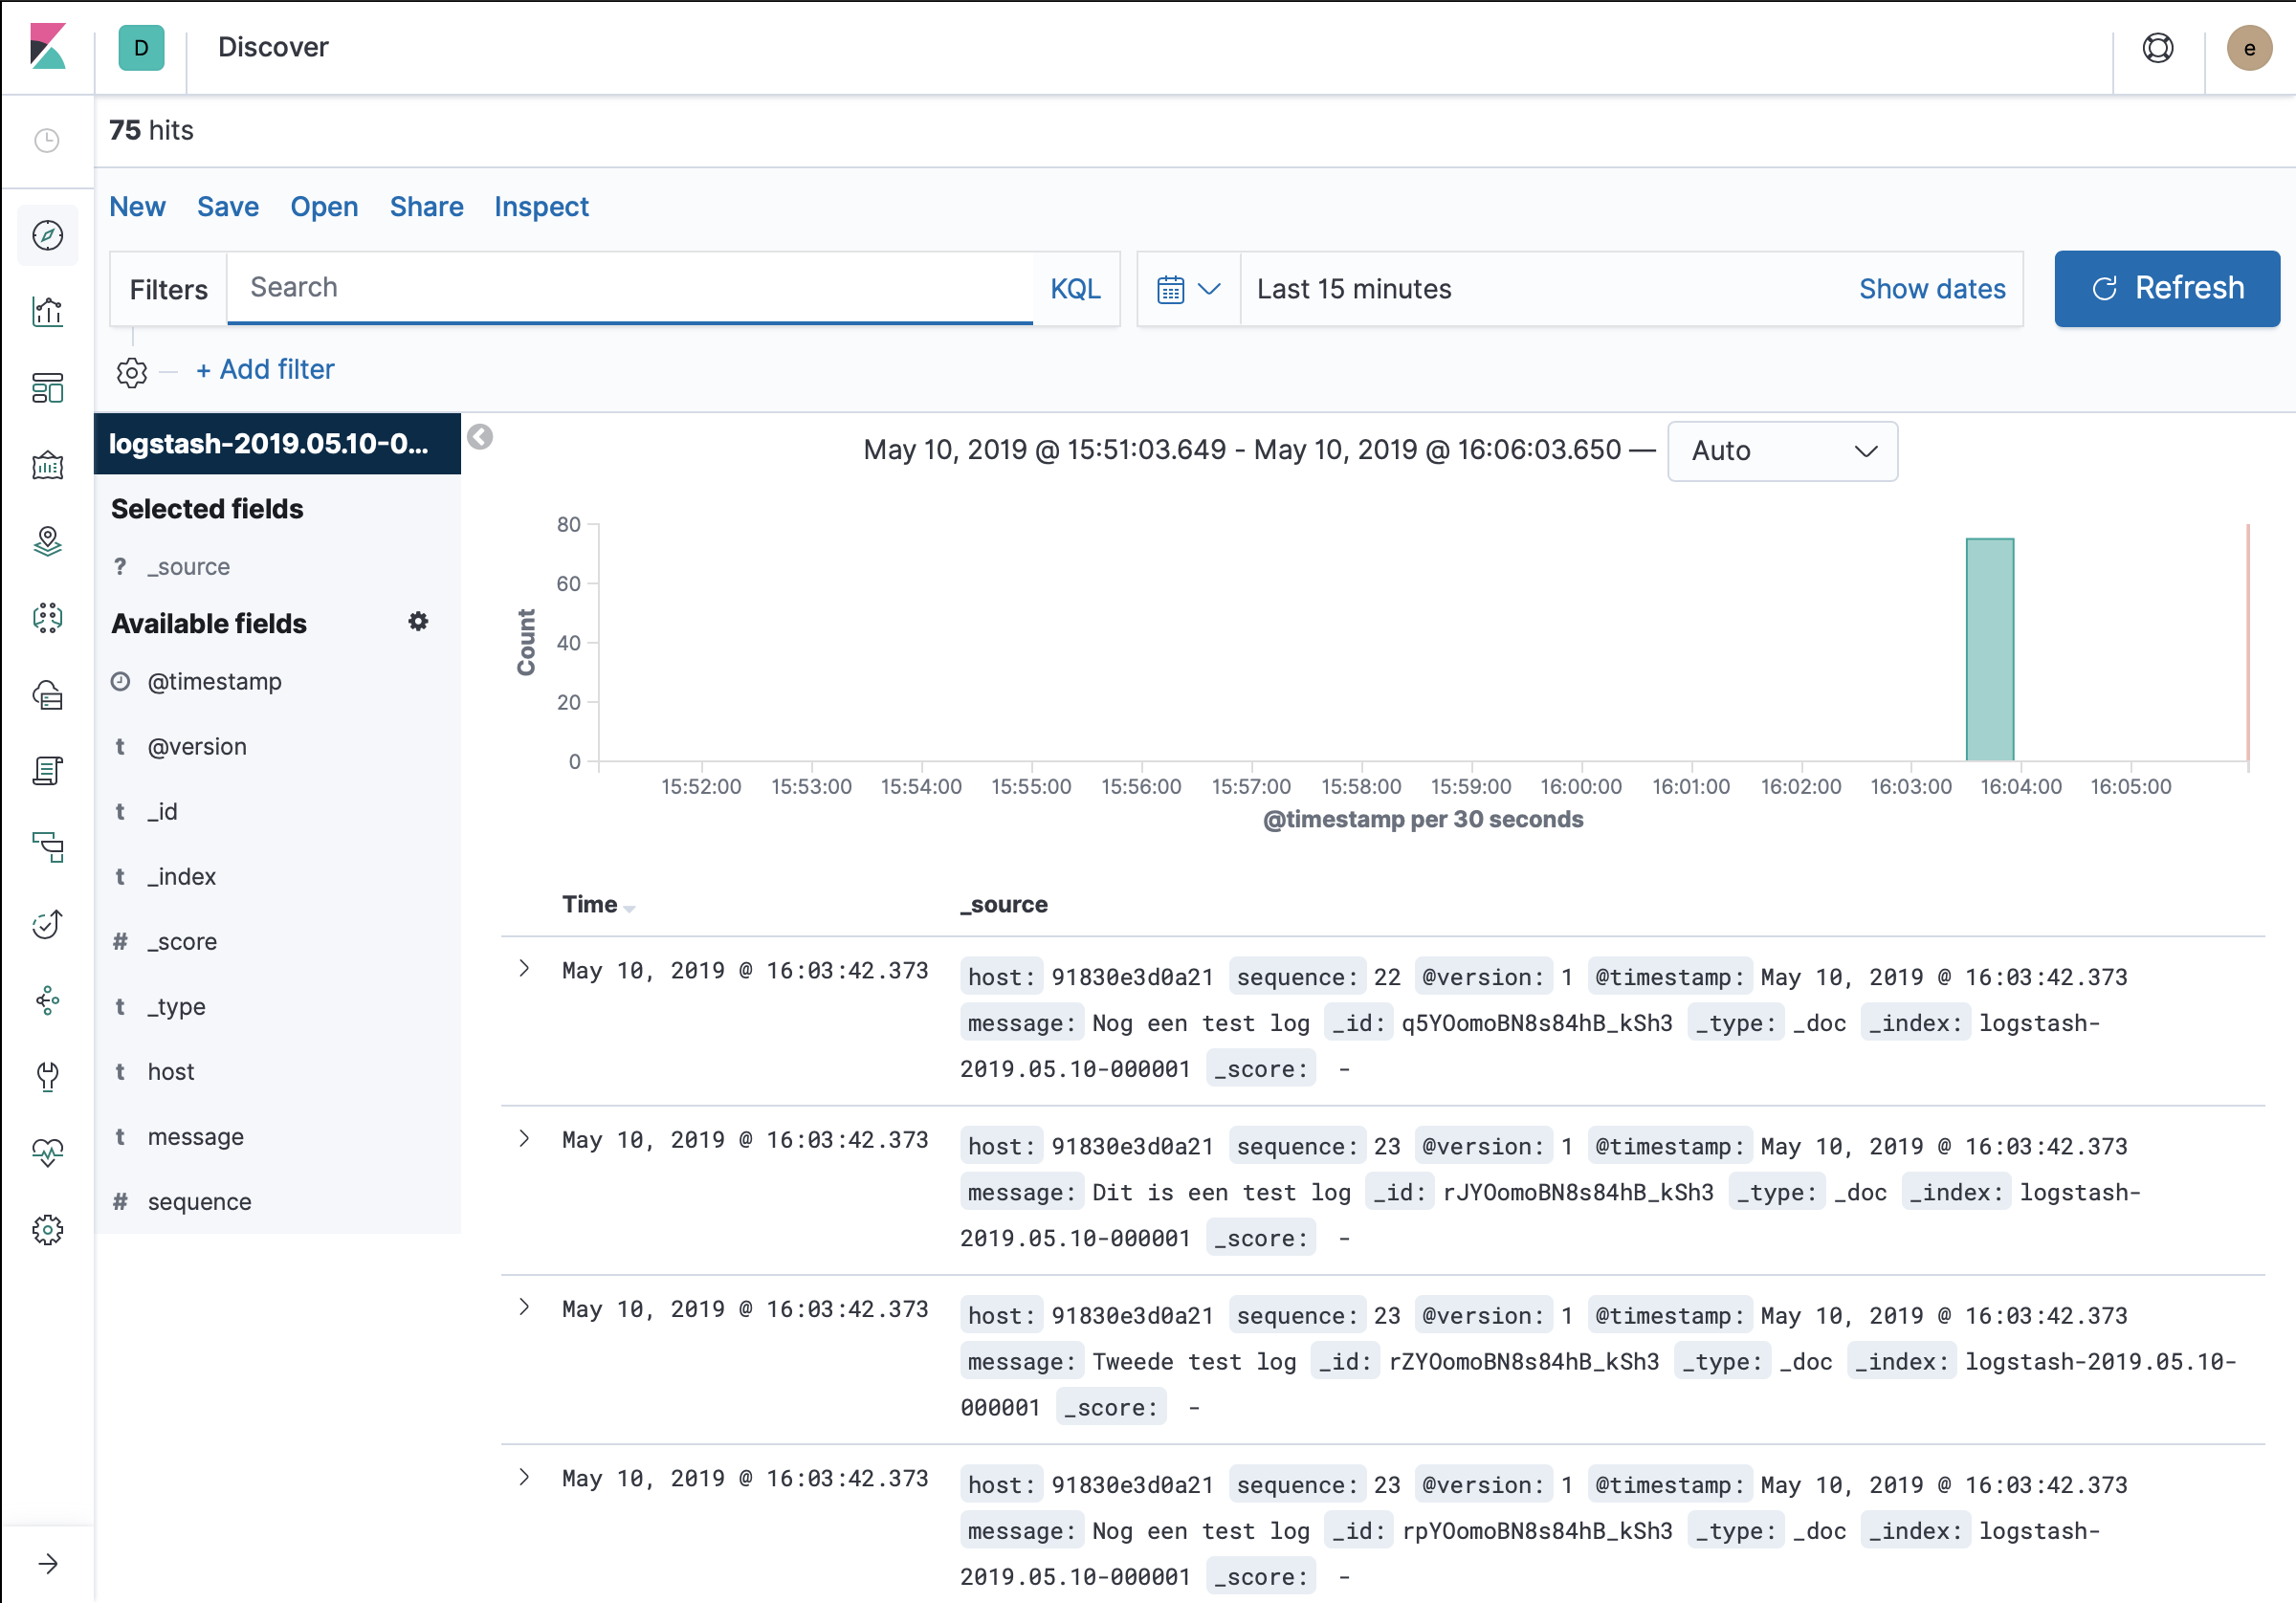
\includegraphics[scale=0.35]{img/ELK-stack-frontend}
    \caption[ELK stack frontend]{ELK stack frontend}
\end{figure}

\subsection{Kubernetes omgeving}

De configuratie van de ELK stack voor Kubernetes is ingewikkelder. Hierbij wordt gebruik gemaakt van een StatefulSet voor de configuratie van Elasticsearch. Dit is lijkt op een gewone Deployment maar heeft enkele verschillen. De belangrijkste is dat elke replica van een Deployment exact hetzelfde is en deze dus uitwisselbaar zijn. In tegenstelling tot alle replicas van een StatefulSet. Deze zijn gebaseerd op eenzelfde configuratie maar zijn niet uitwisselbaar vanwege een unieke, gepersisteerde identifier. StatefulSets worden gebruikt stabiele networken opgebouwd moeten worden met een persistent storage.

De volledige configuratie is buiten de scope van dit onderzoek en zal dus niet besproken worden. De documentatie van Elastic biedt veel ondersteuning bij het opzetten van een eigen Elastic stack.

\section{Requirements}

\subsection{Must have}
\subsubsection{Moet open source zijn}
Voor elk van de onderzochte oplossingen geldt dezelfde score voor deze requirement, namelijk 5. Elk van de componenten waaruit een ELK of Elastic stack bestaat is vrij te verkrijgen en te gebruiken.

\subsubsection{Ondersteuning voor cluster omgevingen zoals Kubernetes}
In de documentatie van Elastic \autocite{elastic} zijn er verschillende links te vinden die een stap voor stap begeleiding geven om deze stack werkende te krijgen. Er zijn ook videos dit nogmaals aantonen dat er een goede ondersteuning is voor Kubernetes.

Om deze redenen zal hiervoor een 4 gegeven voor deze requirement.

\subsubsection{Moet een zo klein mogelijke impact hebben op de servers}
Bij velen is het al geweten dat Elasticsearch een grote impact heeft op het systeem waar het geïmplementeerd is. Een eerste argument hiervoor is de JVM (Java Virtual Machine) waarmee Elasticearch werkt. Deze heeft volgens \cite{elasticheap} een standard minimum heap size van 1GB maar wordt in productie snel omhoog gescaled om ervoor te zorgen dat Elasticsearch functioneel blijft. Dit in combinatie met de best practice voor het installeren op Kubernetes gebruikt door \cite{swidler2018} waarin minstens 3 nodes van Elasticsearch aangemaakt worden, zorgt meteen al voor een hoog RAM gebruik. Een tweede argument hiervoor is de manier waarop Elasticsearch data, in de geval logs, opslaat. Dit gebeurt door middel van volledige indexering waardoor de benodigde opslagruimte groter zal zijn dan andere databanken die indexering vermijden of slecht enkele delen van de data indexeren. 

De combinatie van deze twee argumenten zorgt voor een relatief grote impact op de servers. Daarom krijgt de ELK of Elastic stack een score van 2 voor dit requirement.

\subsubsection{Moet kunnen scalen naargelang de groeiende Kubernetes cluster}
Indien gebruik gemaakt wordt van een DaemonSet voor de configuratie van FileBeats zal het aantal FileBeat containers automatisch gescaled worden bij het aanmaken van nieuwe pods. Wanneer de Kubernetes cluster een bepaalde grootte heeft, zal ook het aantal Elasticsearch nodes groeien. Deze kunnen automatisch gescaled worden met de correcte configuratie.

Indien gesteld wordt dat de oorspronkelijke configuratie correct is gebeurd, kan gesteld worden dat de ELK of Elastic stack automatisch scaled naargelang de groei van de cluster. Daarom krijgt de ELK of Elastic stack een score van 5 voor deze requirement.

\subsection{Should have}
\subsubsection{Moet (relatief) eenvoudig te configureren zijn}
De best practices om Elasticsearch te configureren op Kubernetes zijn dat er minsten 3 nodes aangemaakt moeten worden. 1 master en meerdere data nodes. Er zijn talloze manieren waarop Elasticsearch kan geïnstalleerd worden en heel wat zaken die kunnen mislopen.

FileBeat, Logstash, en Kibana zijn eenvoudig te configureren en vormen geen probleem, zowel lokaal als op Kubernetes. 

Om deze redenen krijgt de ELK of Elastic stack een 2 voor dit requirement

\subsubsection{Moet (relatief) eenvoudig te gebruiken zijn}
De leercurve om gebruik te maken van Elasticsearch is vrij hoog, terwijl de leercurve om gebruik te maken van Kibana relatief laag is.

Voor de requirement krijgt de ELK of Elastic stack een score van 4.

\subsubsection{Moet goed gedocumenteerd zijn}
Dankzij de maturiteit van Elastic is er reeds veel documentatie aanwezig, zowel in de vorm van eigen documentatie en documentatie vanuit de user community. De documentatie van Elastic zelf is zeer uitgebreid voor algemeen gebruik maar voor speciale use cases zal vaak eerder documentatie van de community gebruikt moeten worden.

Voor de requirement krijgt de ELK of Elastic stack een score van 4.

\subsubsection{Moet de logs overzichtelijk kunnen tonen}
De frontend van ELK of Elastic stack is Kibana. Deze zorgt voor een overzichtelijke visualisatie van alle logs. Dankzij de volledige indexering van de data binnen Elasticsearch, is er een uitgebreid filtersysteem waar Kibana gebruik van kan maken. Ook kunnen er deep text queries uitgevoerd worden.

Om deze redenen krijgt de ELK of Elastic stack een 5 voor deze requirement.

\subsubsection{Ondersteuning voor verschillende plugins die data extra kunnen verwerken of naar meerdere locaties kunnen doorsturen}
Filebeat is de logcollector die de logs doorstuurt naar Logstash. Logstash zelf heeft een aantal ondersteunde plugins die gebruikt kunnen worden. Zo kan het een groot aantal inputs verwerken en de data doorsturen naar een groot aantal outputs. Dataverwerking plugins zijn ook beschikbaar maar in mindere mate.

Om deze redenen krijgt de ELK of Elastic stack een 3 voor deze requirement

\subsubsection{Ondersteuning voor visualisatie zoals grafieken}
Kibana voorziet functionaliteit voor het produceren van grafieken. Verschillende soorten grafieken en tellers zijn ondersteund.

Voor de requirement krijgt de ELK of Elastic stack een score van 5.

\subsection{Could have}
\subsubsection{Ondersteuning voor alerts}
Kibana voorziet functionaliteit voor alerts. Deze alerts kunnen via verschillende kanalen verzonden worden. 

Voor de requirement krijgt de ELK of Elastic stack een score van 5.

\section{Resultaten}
Zoals te zien is in tabel~\ref{tab:ELK-resultaten} scoort de ELK stack een 2 op een Must Have requirement, namelijk `Moet een zo klein mogelijke impact hebben op de servers`. Dit wijst erop dat ELK niet geschikt is voor grote clusters. Hoe groter de cluster, hoe groter de impact. Het scoort goed op overzichtelijkheid en functionaliteit. 

Een uitgebreide conclusie is te vinden in Hoofdstuk~\ref{ch:conclusie} Conclusie.

\begin{table}[ht]
    \begin{tabular}{| m{20em} | m{2cm} | m{2cm} | m{2cm} |}
        \hline
        \textbf{Requirement}                                                                                              & \textbf{Score (op 5)} & \textbf{Multiplier} & \textbf{Score met multiplier} \\ \hline
        Moet open source zijn                                                                                             & 5                     & 10                  & 50                            \\ \hline
        Ondersteuning voor cluster omgevingen zoals Kubernetes                                                            & 4                     & 10                  & 40                            \\ \hline
        Moet een zo klein mogelijke impact hebben op de servers                                                           & 2                     & 10                  & 20                            \\ \hline
        Moet kunnen scalen naargelang de groeiende Kubernetes cluster                                                     & 5                     & 10                  & 50                            \\ \hline
        Moet (relatief) eenvoudig te configureren zijn                                                                    & 2                     & 5                   & 10                            \\ \hline
        Moet (relatief) eenvoudig te gebruiken zijn                                                                       & 4                     & 5                   & 20                            \\ \hline
        Moet goed gedocumenteerd zijn                                                                                     & 4                     & 5                   & 20                            \\ \hline
        Moet de logs overzichtelijk kunnen tonen                                                                          & 5                     & 5                   & 25                            \\ \hline
        Ondersteuning voor verschillende plugins die data extra kunnen verwerken of naar meerdere locaties kan doorsturen & 3                     & 5                   & 15                            \\ \hline
        Ondersteuning voor visualisatie zoals grafieken                                                                   & 5                     & 5                   & 25                            \\ \hline
        Ondersteuning voor alerts                                                                                         & 5                     & 1                   & 5                             \\ \hline
        \textbf{Totale score}                                                                                             & 39                    &                     & 280                           \\ \hline
    \end{tabular}
    \caption{ELK resultaten}
    \label{tab:ELK-resultaten}
\end{table}



%%=============================================================================
%% EFK
%%=============================================================================

\chapter{EFK}
\label{ch:EFK}

\section{Installatie en configuratie}
Zoals reeds besproken in Hoofdstuk~\ref{subsec:EFK} EFK, bestaat deze stack uit drie belangrijke componenten.
\begin{itemize}
    \item Fluentd
    \item Elasticsearch
    \item Kibana
\end{itemize}
Fluentd is opgebouwd vanuit een push model. Hierbij pusht de service zelf zijn logs naar Fluentd waar ze verwerkt worden. Om deze demonstratie eenvoudiger te tonen wordt hier gebruik gemaakt van dummy logs als input voor Fluentd. Dit zijn standaard logs die geproduceerd worden door een plugin. 
\subsection{Lokale omgeving}
Om de EFK stack lokaal op te zetten wordt vaak gebruik gemaak van compose up. Compose up laat toe om meerdere docker containers tegelijk op te starten. Alle configuratie om de componenten draaiende te krijgen wordt hierin verwerkt. Voor Fluentd wordt binnenin deze compose-up.yaml (zie Listing 5.1) verwezen naar de fluentd.conf file (zie Listing 5.2). In deze .conf file worden de input en output gedefinieerd. In deze configuratie haalt Fluentd logs binnen van verschillende dummy plugins en stuurt deze automatisch door naar een Elasticsearch instantie alsook naar de stdOut. Belangrijk hierbij is de poort van Elasticsearch welke reeds gedefinieëerd werd in de compose-up.yaml (Listing 5.1).

Door simpelweg deze file uit te voeren zullen alle componenten live draaien in hun eigen Docker container. Wanneer dan naar localhost:5601 gekeken wordt kan men de Kibana frontend van deze stack zien. Na het definiëren van een index zullen op de `Discover` pagina  alle logs van deze index terug te vinden zijn. In Figuur 5.1 is het voorbeeld te zien van hoe Kibana eruit ziet met de gebruikte configuratie.

\begin{lstlisting}[caption=Compose up yaml file for EFK]
version: '2'
services:
    fluentd:
        build: ./fluentd
        volumes:
            - ./fluentd/conf:/fluentd/etc
        links:
            - "elasticsearch"
        ports:
            - "8080:8080"
    
    elasticsearch:
        image: docker.elastic.co/elasticsearch/elasticsearch:6.2.4
        environment:
            discovery.type: single-node
        expose:
            - 9200
        ports:
            - "9200:9200"
        
    kibana:
        image: docker.elastic.co/kibana/kibana:6.2.4
        links:
            - "elasticsearch"
        ports:
            - "5601:5601"
\end{lstlisting}

\begin{lstlisting}[caption=Fluentd config file]
<source>
    @type dummy
    dummy {"info":"message 1"}
    tag dummy 1
</source>

<source>
    @type dummy
    dummy {"warning":"message 2"}
    tag dummy 2
</source>

<source>
    @type dummy
    dummy {"error":"message 3"}
    tag dummy 3
</source>

<match **>
    @type copy
    <store>
        @type elasticsearch
        host elasticsearch
        port 9200
        index_name fluentd
        type_name fluentd
        logstash_format true
        logstash_prefix fluentd
        logstash_dateformat %Y%m%d
        include_tag_key true
        tag_key @log_name
        flush_interval 1s
    </store>
    <store>
        @type stdout
    </store>
</match>
\end{lstlisting}

\begin{figure}[ht]
    \centering
    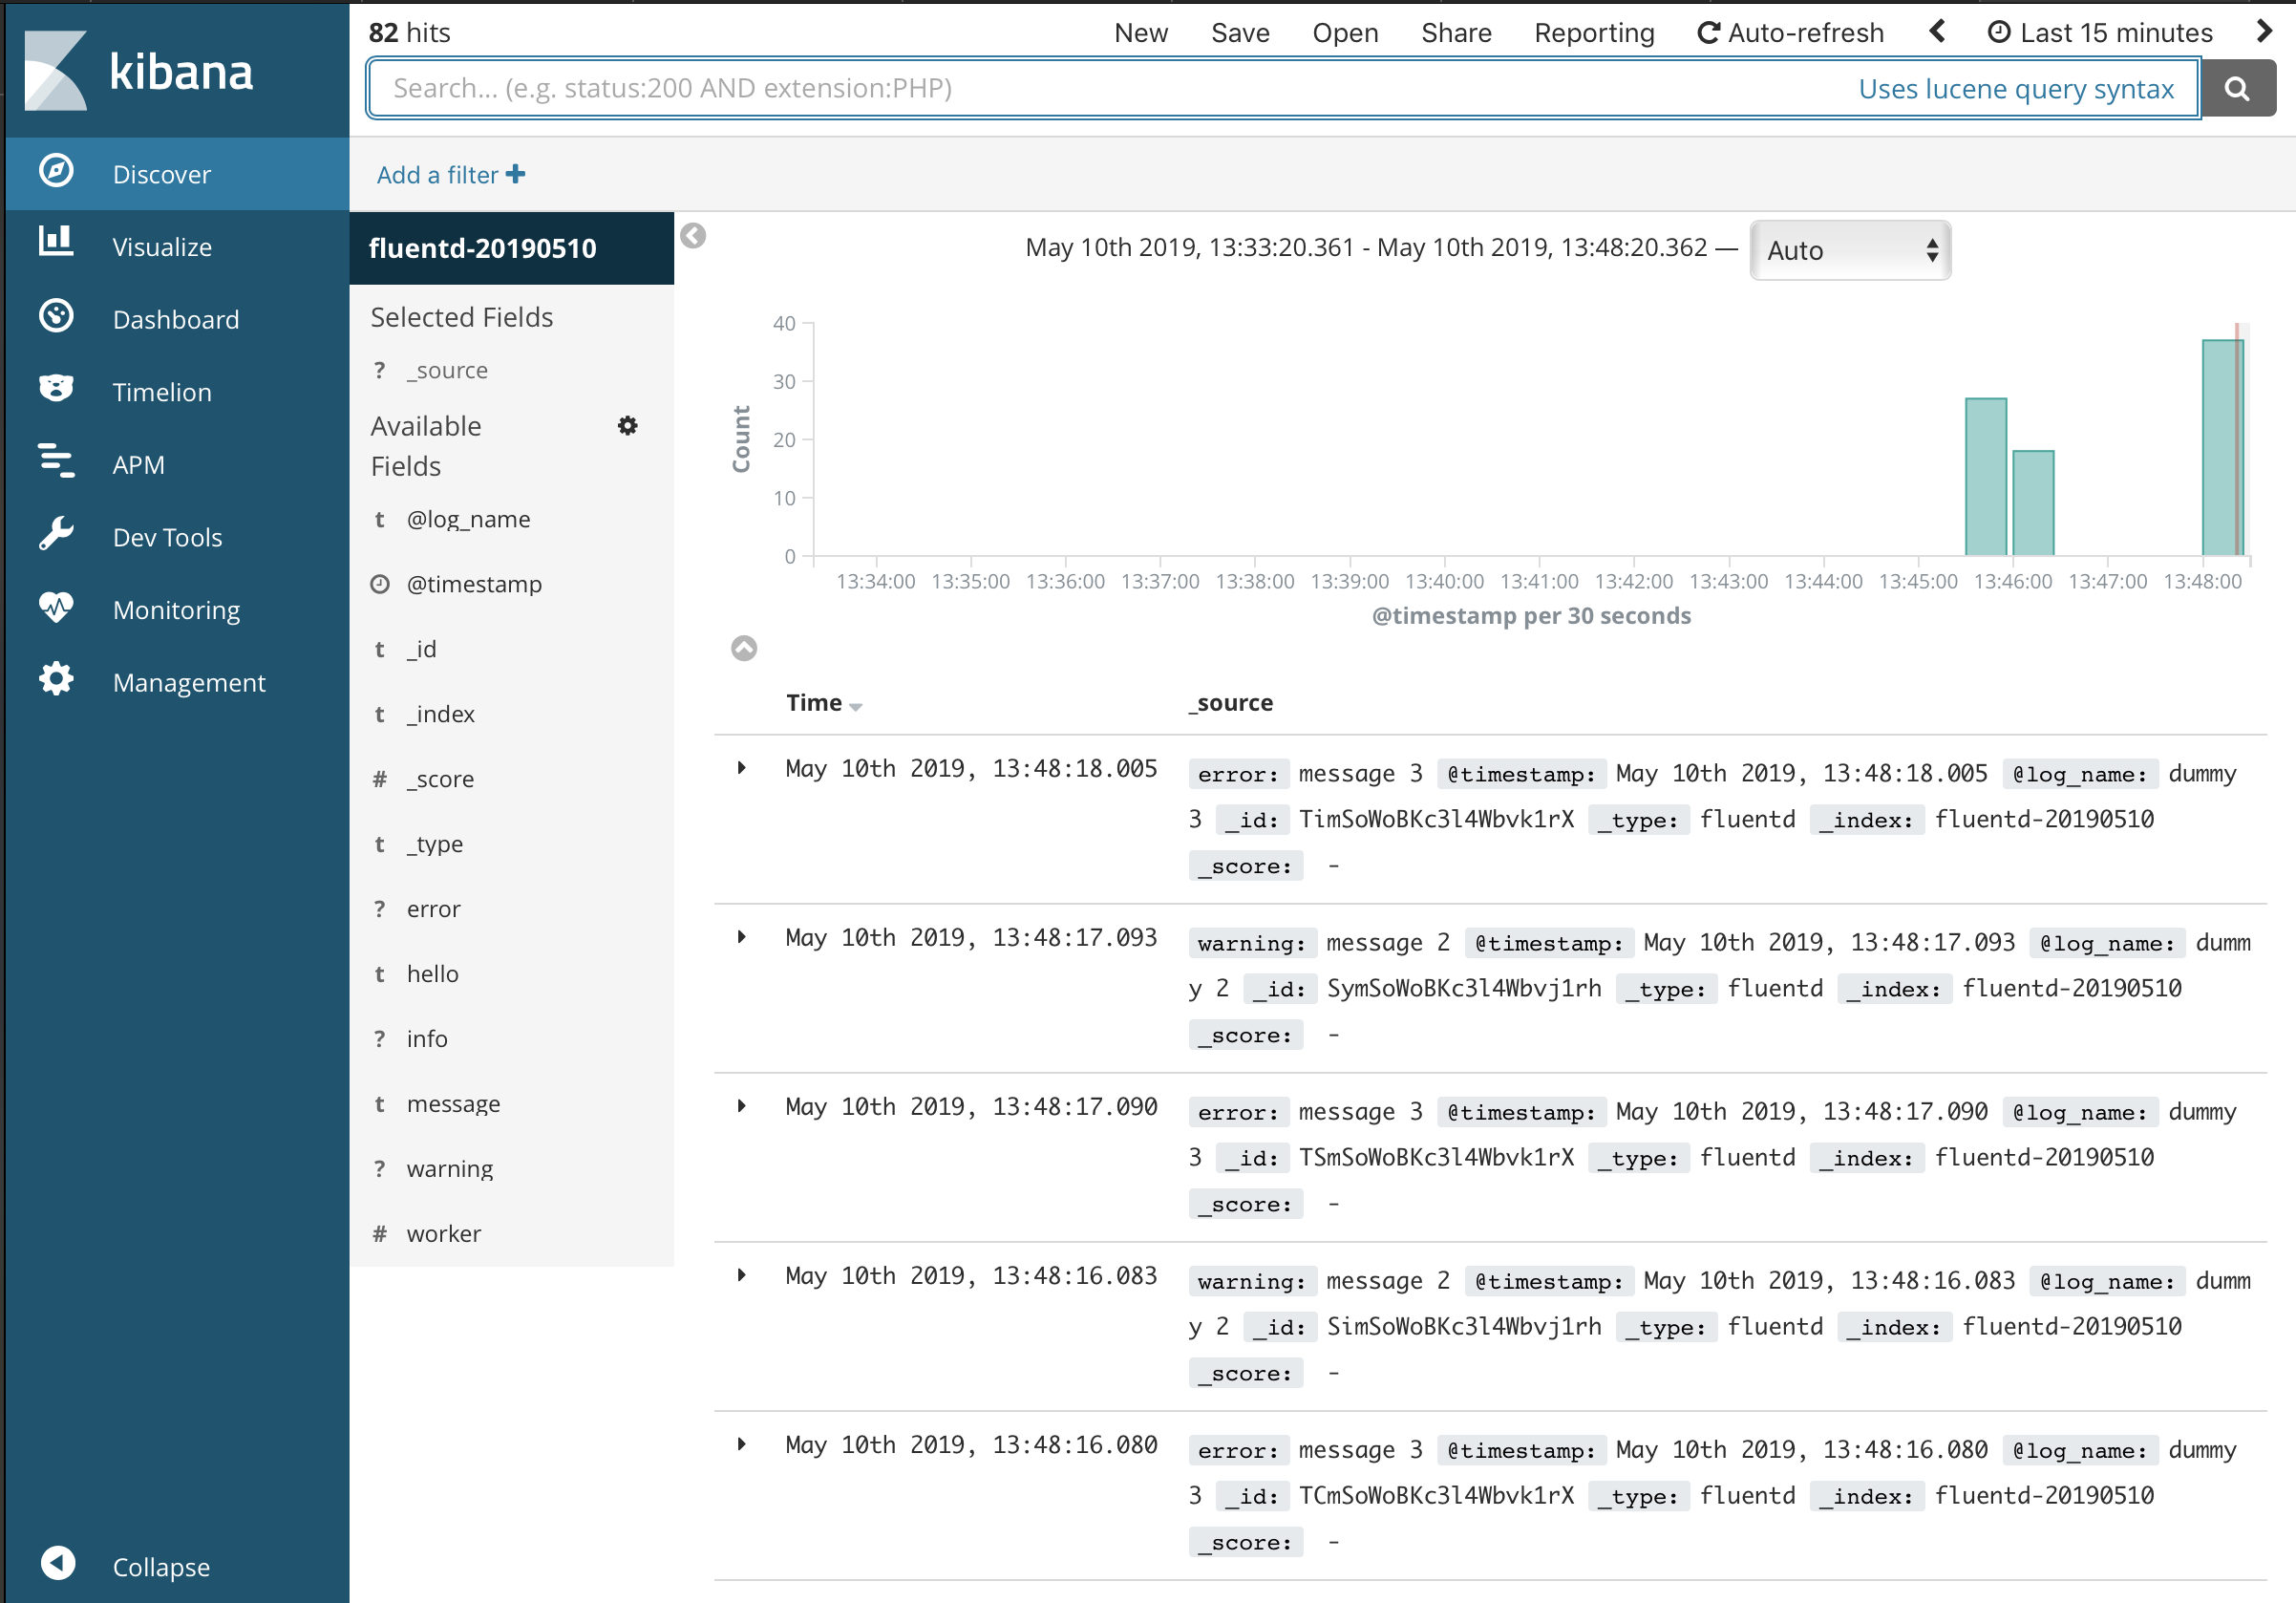
\includegraphics[scale=0.35]{img/EFK-stack}
    \caption[EFK stack frontend]{EFK stack frontend}
\end{figure}

\subsection{Kubernetes omgeving}
De configuratie van de EFK stack voor Kubernetes is ingewikkelder. Hierbij wordt, net zoals bij de ELK stack, gebruik gemaakt van een StatefulSet voor de configuratie van Elasticsearch.

In het artikel van \cite{jetha2018} wordt uitgebreid besproken hoe de EFK stack kan opgezet worden. 

\section{Requirements}

\subsection{Must have}
\subsubsection{Moet open source zijn}
Voor elk van de onderzochte oplossingen geldt dezelfde score voor deze requirement, namelijk 5. Elk van de componenten waaruit een EFK stack bestaat, namelijk Elastischsearch, Fluentd, en Kibana, is vrij te verkrijgen en te gebruiken.

\subsubsection{Ondersteuning voor cluster omgevingen zoals Kubernetes}
Bij de EFK stack geldt een soortgelijke uitleg als bij de ELK of Elastic stack. Dezelfde documentatie welke gebruikt kan worden voor de ELK of elastic stack kan gebruikt worden voor de EFK stack. Met bijkomende documentatie over het configureren van zowel Fluentd als Fluentbit. 

Deze argumenten leiden tot een score van 4 voor de EFK stack.

\subsubsection{Moet een zo klein mogelijke impact hebben op de servers}
Zoals eerder besproken in de sectie~\ref{sec:logging-solutions} heeft deze oplossing een minimale impact op de servers wanneer in acht wordt genomen dat er gebruik wordt gemaakt van Elastiscsearch als databank. Het enige verschilpunt met ELK is dus het gebruik van Fluentd en Fluentbit. Wanneer deze op een correct manier geconfigureerd zijn, zal deze zuiniger zijn op vlak van geheugen gebruik (zie ~\ref{subsec:EFK}, vergelijking tussen Fluentd en Logstash). 

Er blijft wel gebruik gemaakt worden van Elasticsearch waardoor de score voor EFK niet hoger dan 3 kan zijn.

\subsubsection{Moet kunnen scalen naargelang de groeiende Kubernetes cluster}
Ook hier moet gebruik gemaakt worden van een DaemonSet voor de configuratie van Fluentbit om een automatische scaling te garanderen. 

Indien gesteld wordt dat de oorspronkelijke configuratie correct is gebeurd, kan gesteld worden dat de EFK stack automatisch kan scalen naargelang de groei van de cluster. Daarom krijgt EFK een score van 5 voor dit requirement.

\subsection{Should have}
\subsubsection{Moet (relatief) eenvoudig te configureren zijn}
Voor EFK geldt eenzelfde uitleg als de ELK of Elastic stack voor dit requirement. De configuratie van Elastischsearch is ingewikkeld en neemt veel tijd in beslag om correct uit te voeren. 

Fluentd en Fluentbit zijn relatief eenvoudig te configureren en vormen geen probleem voor deze requirement. Wel moet vermeld worden dat de configuratie van Fluentd en Fluentbit moeilijker is dan deze van Logstash en Filebeat \autocite{harikumar2018}.

Om deze redenen krijgt EFK, net als de ELK of Elastic stack, een 2 voor dit requirement.

\subsubsection{Moet (relatief) eenvoudig te gebruiken zijn}
Voor EFK geldt eenzelfde uitleg als de ELK of Elastic stack voor dit requirement. Er geldt een hoge leercurve voor Elasticsearch maar wanneer er sprake is van basis use cases zoals simpele log visualatie in de vorm van simpele grafieken, zal het gebruik van Kibana vanzelfsprekend zijn.

Om deze redenen krijgt EFK, net als de ELK of Elastic stack, een 4 voor dit requirement.

\subsubsection{Moet goed gedocumenteerd zijn}
Voor EFK geldt eenzelfde uitleg als de ELK of Elastic stack voor dit requirement. De Elasticsearch documentatie is zeer uitgebreid. De documentatie van Fluentd en Fluentbit is ook talrijk aanwezig in verschillende officiele en community bronnen.

Voor dit requirement krijgt EFK net als de EFK of Elastic stack een score van 4.

\subsubsection{Moet de logs overzichtelijk kunnen tonen}
Voor EFK geldt eenzelfde uitleg als de ELK of Elastic stack voor dit requirement. De frontend voor de EFK stack is Kibana. De EFK stack beschikt over dezelfde voordelen als de ELK of Elasticstack.

Om deze reden krijgt EFK dezelfde score als de ELK of Elastic stack, namelijk 5.

\subsubsection{Ondersteuning voor verschillende plugins die data extra kunnen verwerken of naar meerdere locaties kunnen doorsturen}
Bij de EFK stack wordt gebruik gemaakt van Fluentbit om de logs te verzamelen en door te sturen naar Fluentd. Deze verwerkt de logs en stuurt deze door naar Elasticsearch. Zowel Fluentbit als Fluentd beschikken over een groot aantal plugins om data te verwerken en door te sturen naar meerdere locaties.

Voor de requirement krijgt de EFK stack een score van 5.

\subsubsection{Ondersteuning voor visualisatie zoals grafieken}
Voor EFK geldt eenzelfde uitleg als de ELK of Elastic stack voor dit requirement. Door het gebruik van Kibana kan gesteld worden dat EFK een uitstekende visualisatie heeft voor alle logs.

Voor de requirement krijgt de EFK stack een score van 5.

\subsection{Could have}
\subsubsection{Ondersteuning voor alerts}
Voor EFK geldt eenzelfde uitleg als de ELK of Elastic stack voor dit requirement. Dankzij Kibana voorziet de EFK stack ondersteuning voor alerts. Deze kunnen via verschillende kanalen verzonden worden.

Voor de requirement krijgt de EFK stack een score van 5.

\section{Resultaten}

Zoals te zien is in tabel~\ref{tab:EFK-resultaten}, scoort EFK een hoge score. Het scoort goed bij de Must Haves en kan dus als een geschikte oplossing beschouwd worden. Het laagste cijfer is een 2, wat gegeven is voor de requirement `Moet (relatief) eenvoudig te configureren zijn`, dit is te wijten aan de complexiteit die gepaard gaat met Elasticsearch. Het scoort de maximale score op verschillende requirements, dit is vooral te wijten aan het gebruik van Kibana.

Een uitgebreide conclusie is te vinden in Hoofdstuk~\ref{ch:conclusie} Conclusie.

\begin{table}[ht]
    \begin{tabular}{| m{20em} | m{2cm} | m{2cm} | m{2cm} | }
        \hline
        \textbf{Requirement}                                                                                              & \textbf{Score (op 5)} & \textbf{Multiplier} & \textbf{Score met multiplier} \\ \hline
        Moet open source zijn                                                                                             & 5                     & 10                  & 50                            \\ \hline
        Ondersteuning voor cluster omgevingen zoals Kubernetes                                                            & 4                     & 10                  & 40                            \\ \hline
        Moet een zo klein mogelijke impact hebben op de servers                                                           & 3                     & 10                  & 30                            \\ \hline
        Moet kunnen scalen naargelang de groeiende Kubernetes cluster                                                     & 5                     & 10                  & 50                            \\ \hline
        Moet (relatief) eenvoudig te configureren zijn                                                                    & 2                     & 5                   & 10                            \\ \hline
        Moet (relatief) eenvoudig te gebruiken zijn                                                                       & 4                     & 5                   & 20                            \\ \hline
        Moet goed gedocumenteerd zijn                                                                                     & 4                     & 5                   & 20                            \\ \hline
        Moet de logs overzichtelijk kunnen tonen                                                                          & 5                     & 5                   & 25                            \\ \hline
        Ondersteuning voor verschillende plugins die data extra kunnen verwerken of naar meerdere locaties kan doorsturen & 5                     & 5                   & 25                            \\ \hline
        Ondersteuning voor visualisatie zoals grafieken                                                                   & 5                     & 5                   & 25                            \\ \hline
        Ondersteuning voor alerts                                                                                         & 5                     & 1                   & 5                             \\ \hline
        \textbf{Totale score}                                                                                             & 47                    &                     & 300                           \\ \hline
    \end{tabular}
    \caption{EFK resultaten}
    \label{tab:EFK-resultaten}
\end{table}
%%=============================================================================
%% Graylog
%%=============================================================================

\chapter{Graylog}
\label{ch:graylog}

\section{Installatie en configuratie}

\subsection{Lokale omgeving}
De opzet van Graylog in een lokale omgeving gebeurt relatief eenvoudig. De uitstekende documentatie van Graylog zorgt ervoor dat er meer dan een manier is om dit te doen. De manier waarop hier tewerk is gegaan, gaat als volgt. Er werd een docker-compose.yaml file aangemaakt met de configuratie die te zien is in Listing 6.1. Deze docker-compose definieert drie services, MongoDB, Elasticsearch, en Graylog. MongoDB is verantwoordelijk voor het opslaan van de metadata. Elasticsearch is de database waar alle logs naartoe worden gestuurd. Graylog is de frontend waar de logs zullen getoond worden.

Met het commando `docker-compose up` wordt deze configuratie uitgevoerd en zal de Graylog server samen met Elasticsearch en MongoDb lokaal draaien. Daarna kunnen er logs naar Elasticsearch gestuurd worden. In dit voorbeeld is gekozen voor Fluentd omdat deze een plugin bezit dit GELF als output kan definiëren. GELF werd reeds uitgelegd in ~\ref{subsec:graylog} Graylog. Dit configuratie van Fluentd is te zien in Listing 6.2. Deze configuratie wordt gebruikt bij het uitvoeren van Fluentd in het commando dat te zien is in Listing 6.3.

\begin{lstlisting}[caption=docker-compose.yaml]
   version: '2'
   services:
       # MongoDB: https://hub.docker.com/_/mongo/
       mongodb:
           image: mongo:3
               # Elasticsearch: https://www.elastic.co/guide/en/elasticsearch/reference/6.6/docker.html
           elasticsearch:
               image: docker.elastic.co/elasticsearch/elasticsearch-oss:6.6.1
           environment:
               - http.host=0.0.0.0
               - transport.host=localhost
               - network.host=0.0.0.0
               - "ES_JAVA_OPTS=-Xms512m -Xmx512m"
           ulimits:
           memlock:
           soft: -1
           hard: -1
           mem_limit: 1g
           # Graylog: https://hub.docker.com/r/graylog/graylog/
       graylog:
           image: graylog/graylog:3.0
           environment:
               # CHANGE ME (must be at least 16 characters)!
               - GRAYLOG_PASSWORD_SECRET=somepasswordpepper
               # Password: admin
               - GRAYLOG_ROOT_PASSWORD_SHA2=8c6976e5b5410415bde908bd4dee15dfb167a9c873fc4bb8a81f6f2ab448a918
               - GRAYLOG_HTTP_EXTERNAL_URI=http://127.0.0.1:9000/
           links:
               - mongodb:mongo
               - elasticsearch
           depends_on:
               - mongodb
               - elasticsearch
           ports:
               # Graylog web interface and REST API
               - 9000:9000
               # Syslog TCP
               - 1514:1514
               # Syslog UDP
               - 1514:1514/udp
               # GELF TCP
               - 12201:12201
               # GELF UDP
               - 12201:12201/udp
\end{lstlisting}
\begin{lstlisting}[caption=Fluentd configuratie]
<source>
    @type dummy
    dummy {"info":"message 1"}
    tag dummy 1
</source>

<source>
    @type dummy
    dummy {"warning":"message 2"}
    tag dummy 2
</source>

<source>
    @type dummy
    dummy {"error":"message 3"}
    tag dummy 3
</source>

<match **>
    type gelf
    host 0.0.0.0
    port 12201
    <buffer>
        flush_interval 5s
    </buffer>
</match>
\end{lstlisting}
\begin{lstlisting}[caption=Uitvoeren van Fluentd met configuratie]
$ fluentd -c ./fluent/fluent.conf
\end{lstlisting}

Nadat Graylog en Fluentd volledig zijn uitgerold, kan naar localhost:9000 gesurft worden om de Web Interface te zien. Hier moet eerst nog ingelogd worden met de inloggevens: \begin{itemize}
   \item username: admin
   \item password: admin
\end{itemize}
Na het inloggen kan bij systeem->inputs een databank ingegeven worden waar op zoek wordt gegaan naar logs. Dit scherm is te zien in Figuur 6.3. Hier moet dezelfde poort gebruikt worden als deze gedefinieerd in de docker-compos configuratie van Graylog. Na het toevoegen van een input zijn de verstuurde logs te zien op de startpagina, zie Figuur 6.1. Wanneer extra details van een log gewenst zijn, kan doorgeklikt worden hierop om een detailscherm te verkijgen, zie Figuur 6.2.

\begin{figure}[ht]
    \centering
    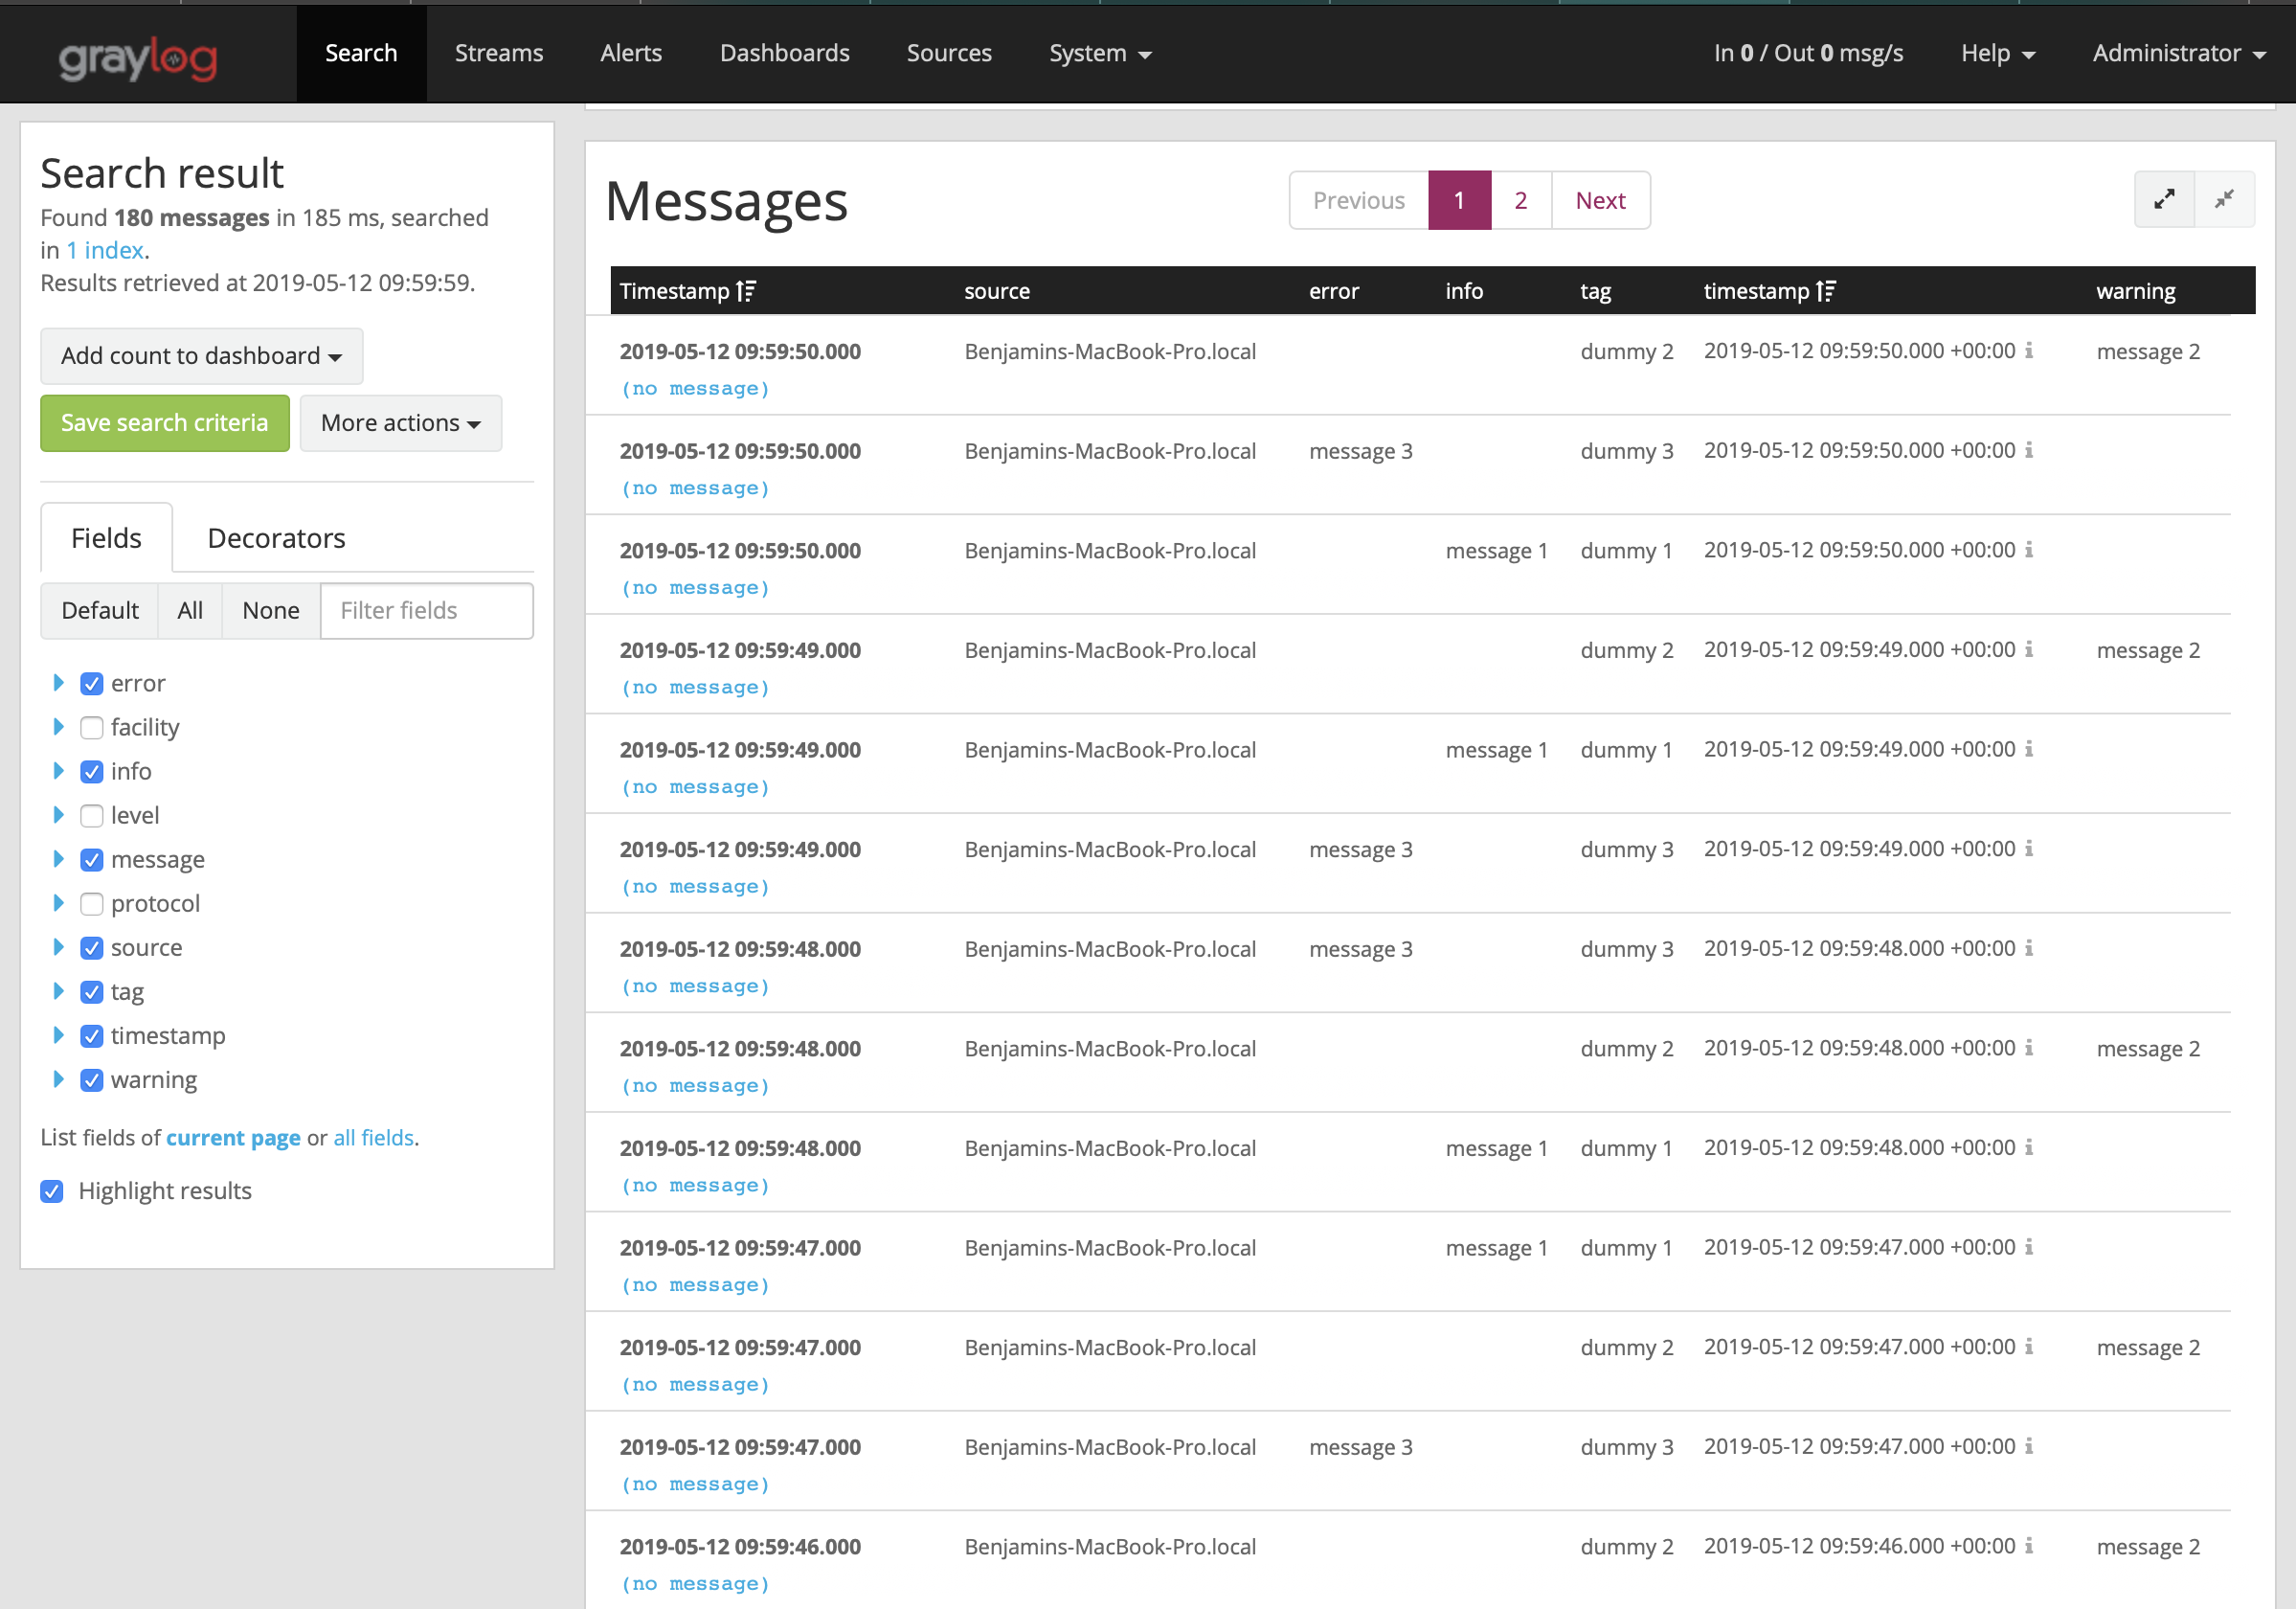
\includegraphics[scale=0.35]{img/graylog_overview}
    \caption[Graylog stack frontend]{Graylog stack frontend}
\end{figure}

\begin{figure}[ht]
    \centering
    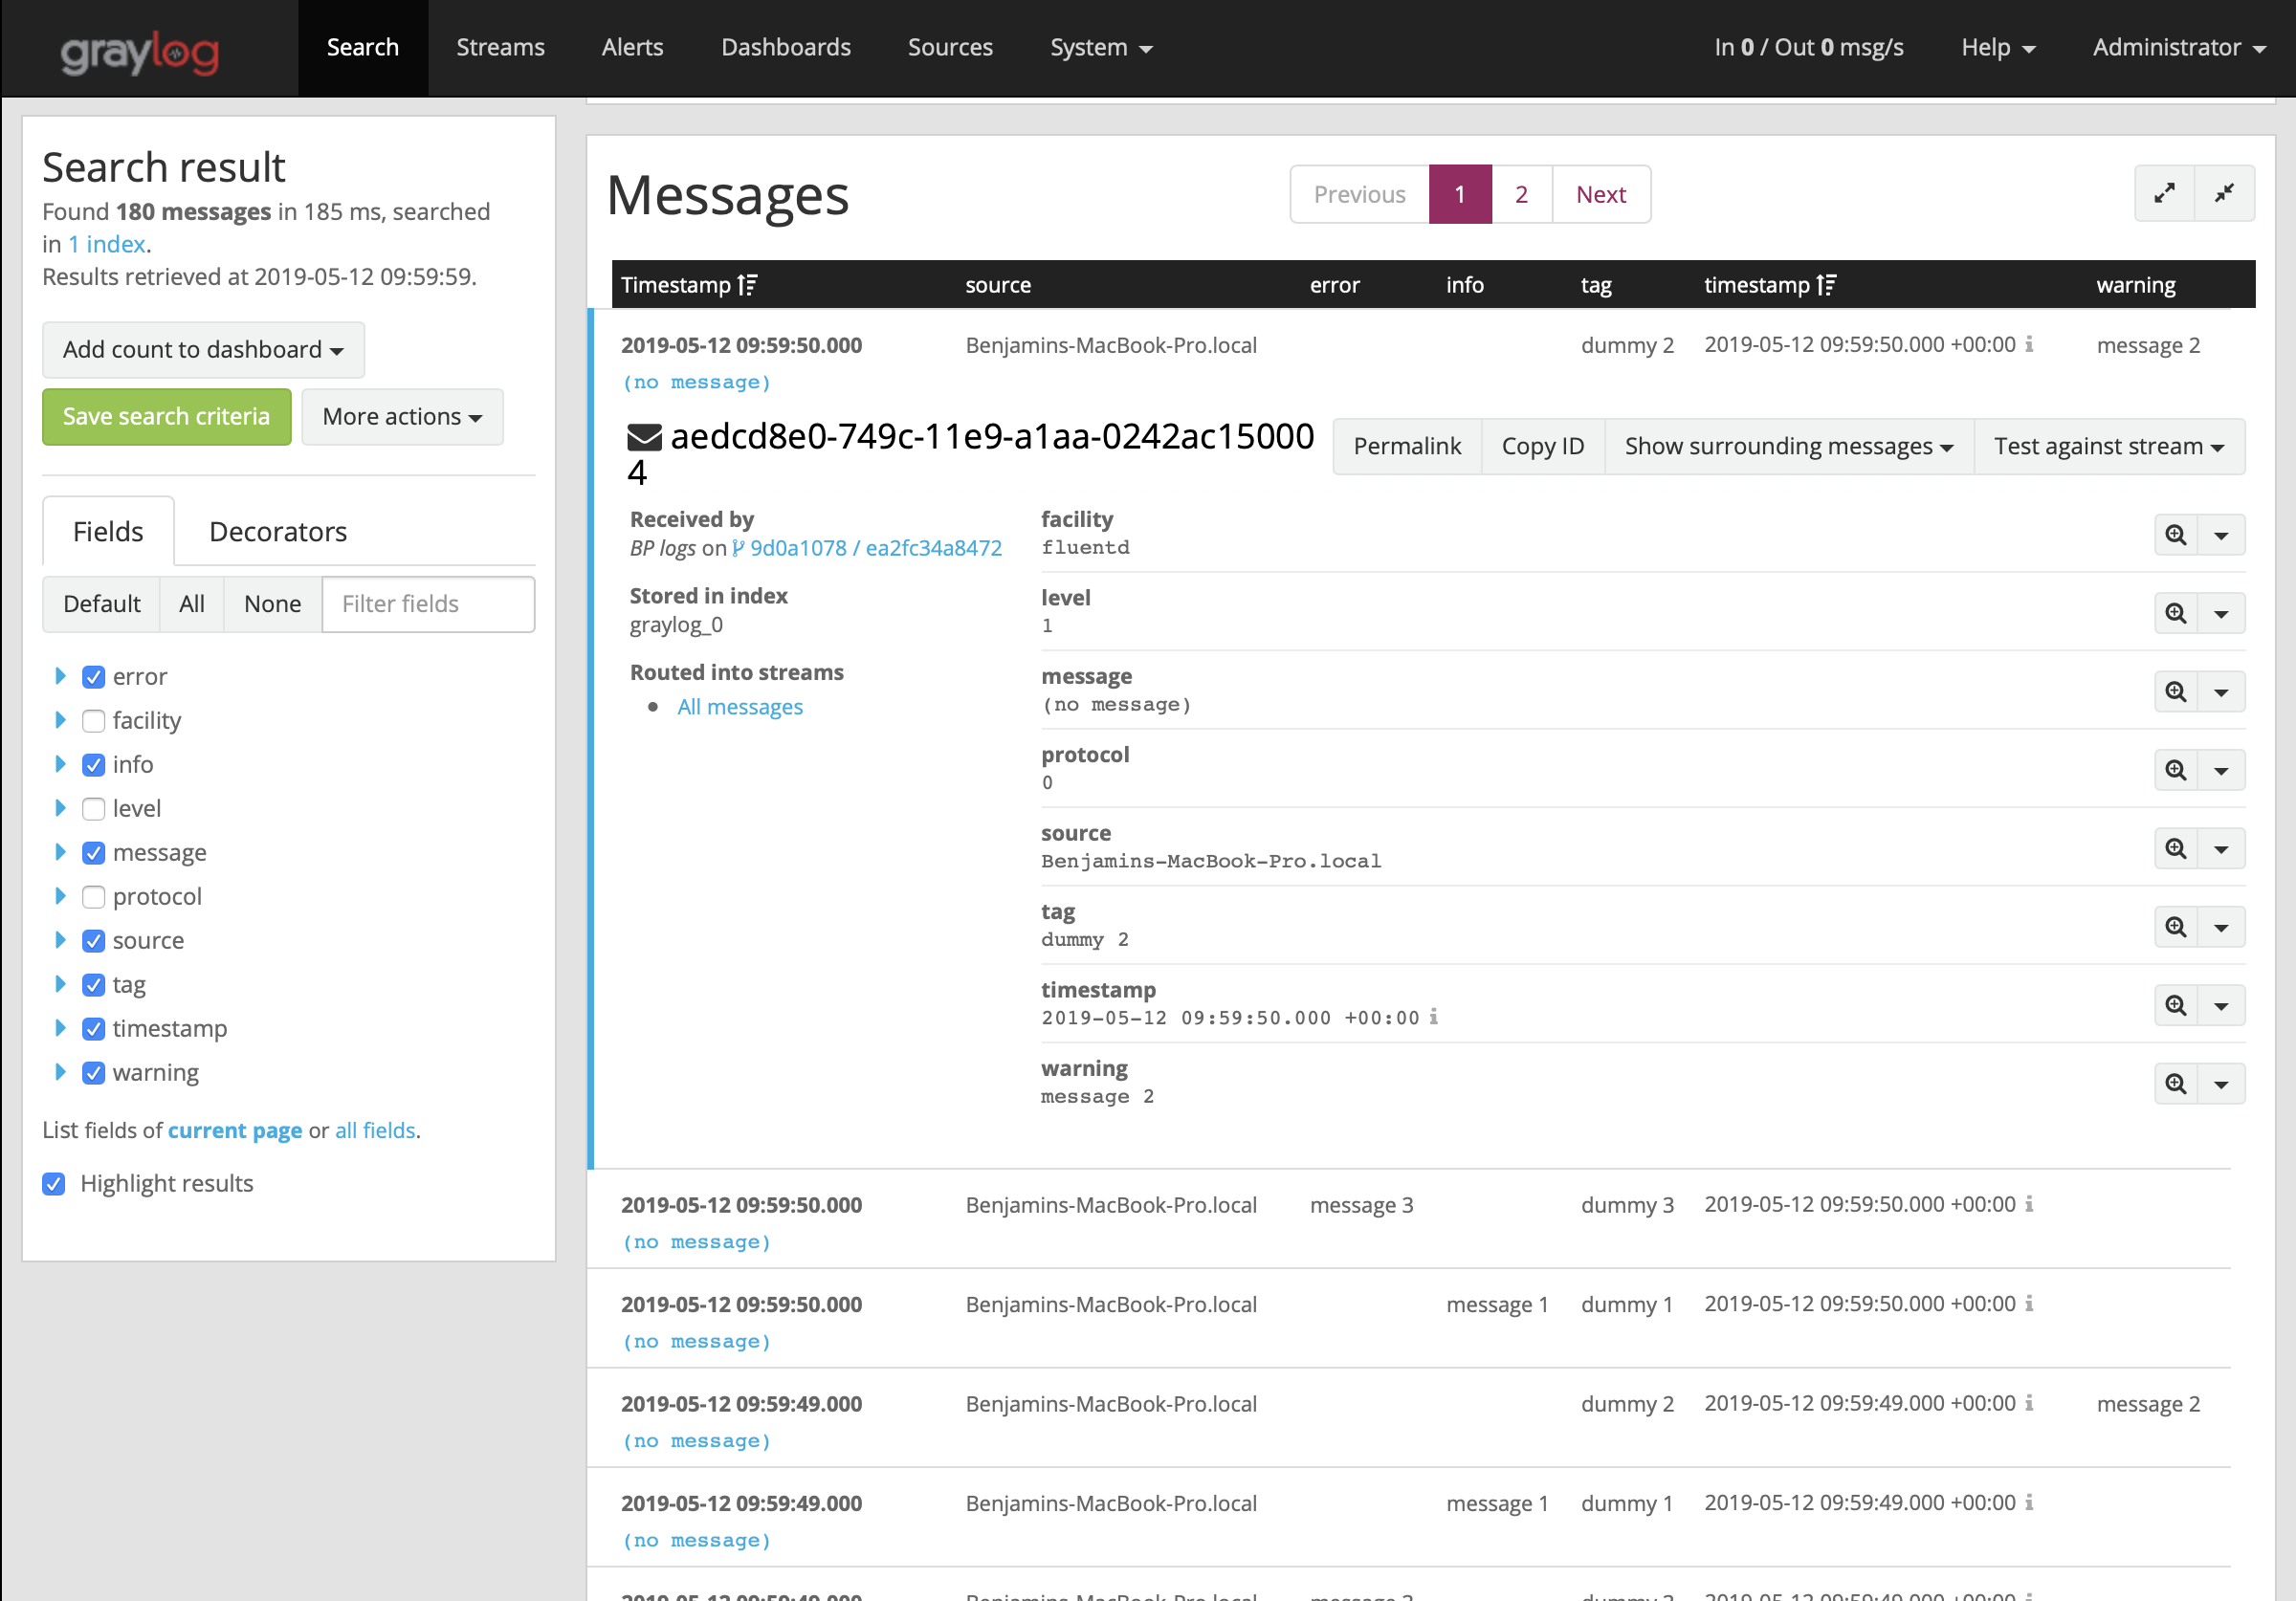
\includegraphics[scale=0.35]{img/graylog_detail}
    \caption[Graylog log detailscherm]{Graylog log detail}
\end{figure}

\begin{figure}[ht]
    \centering
    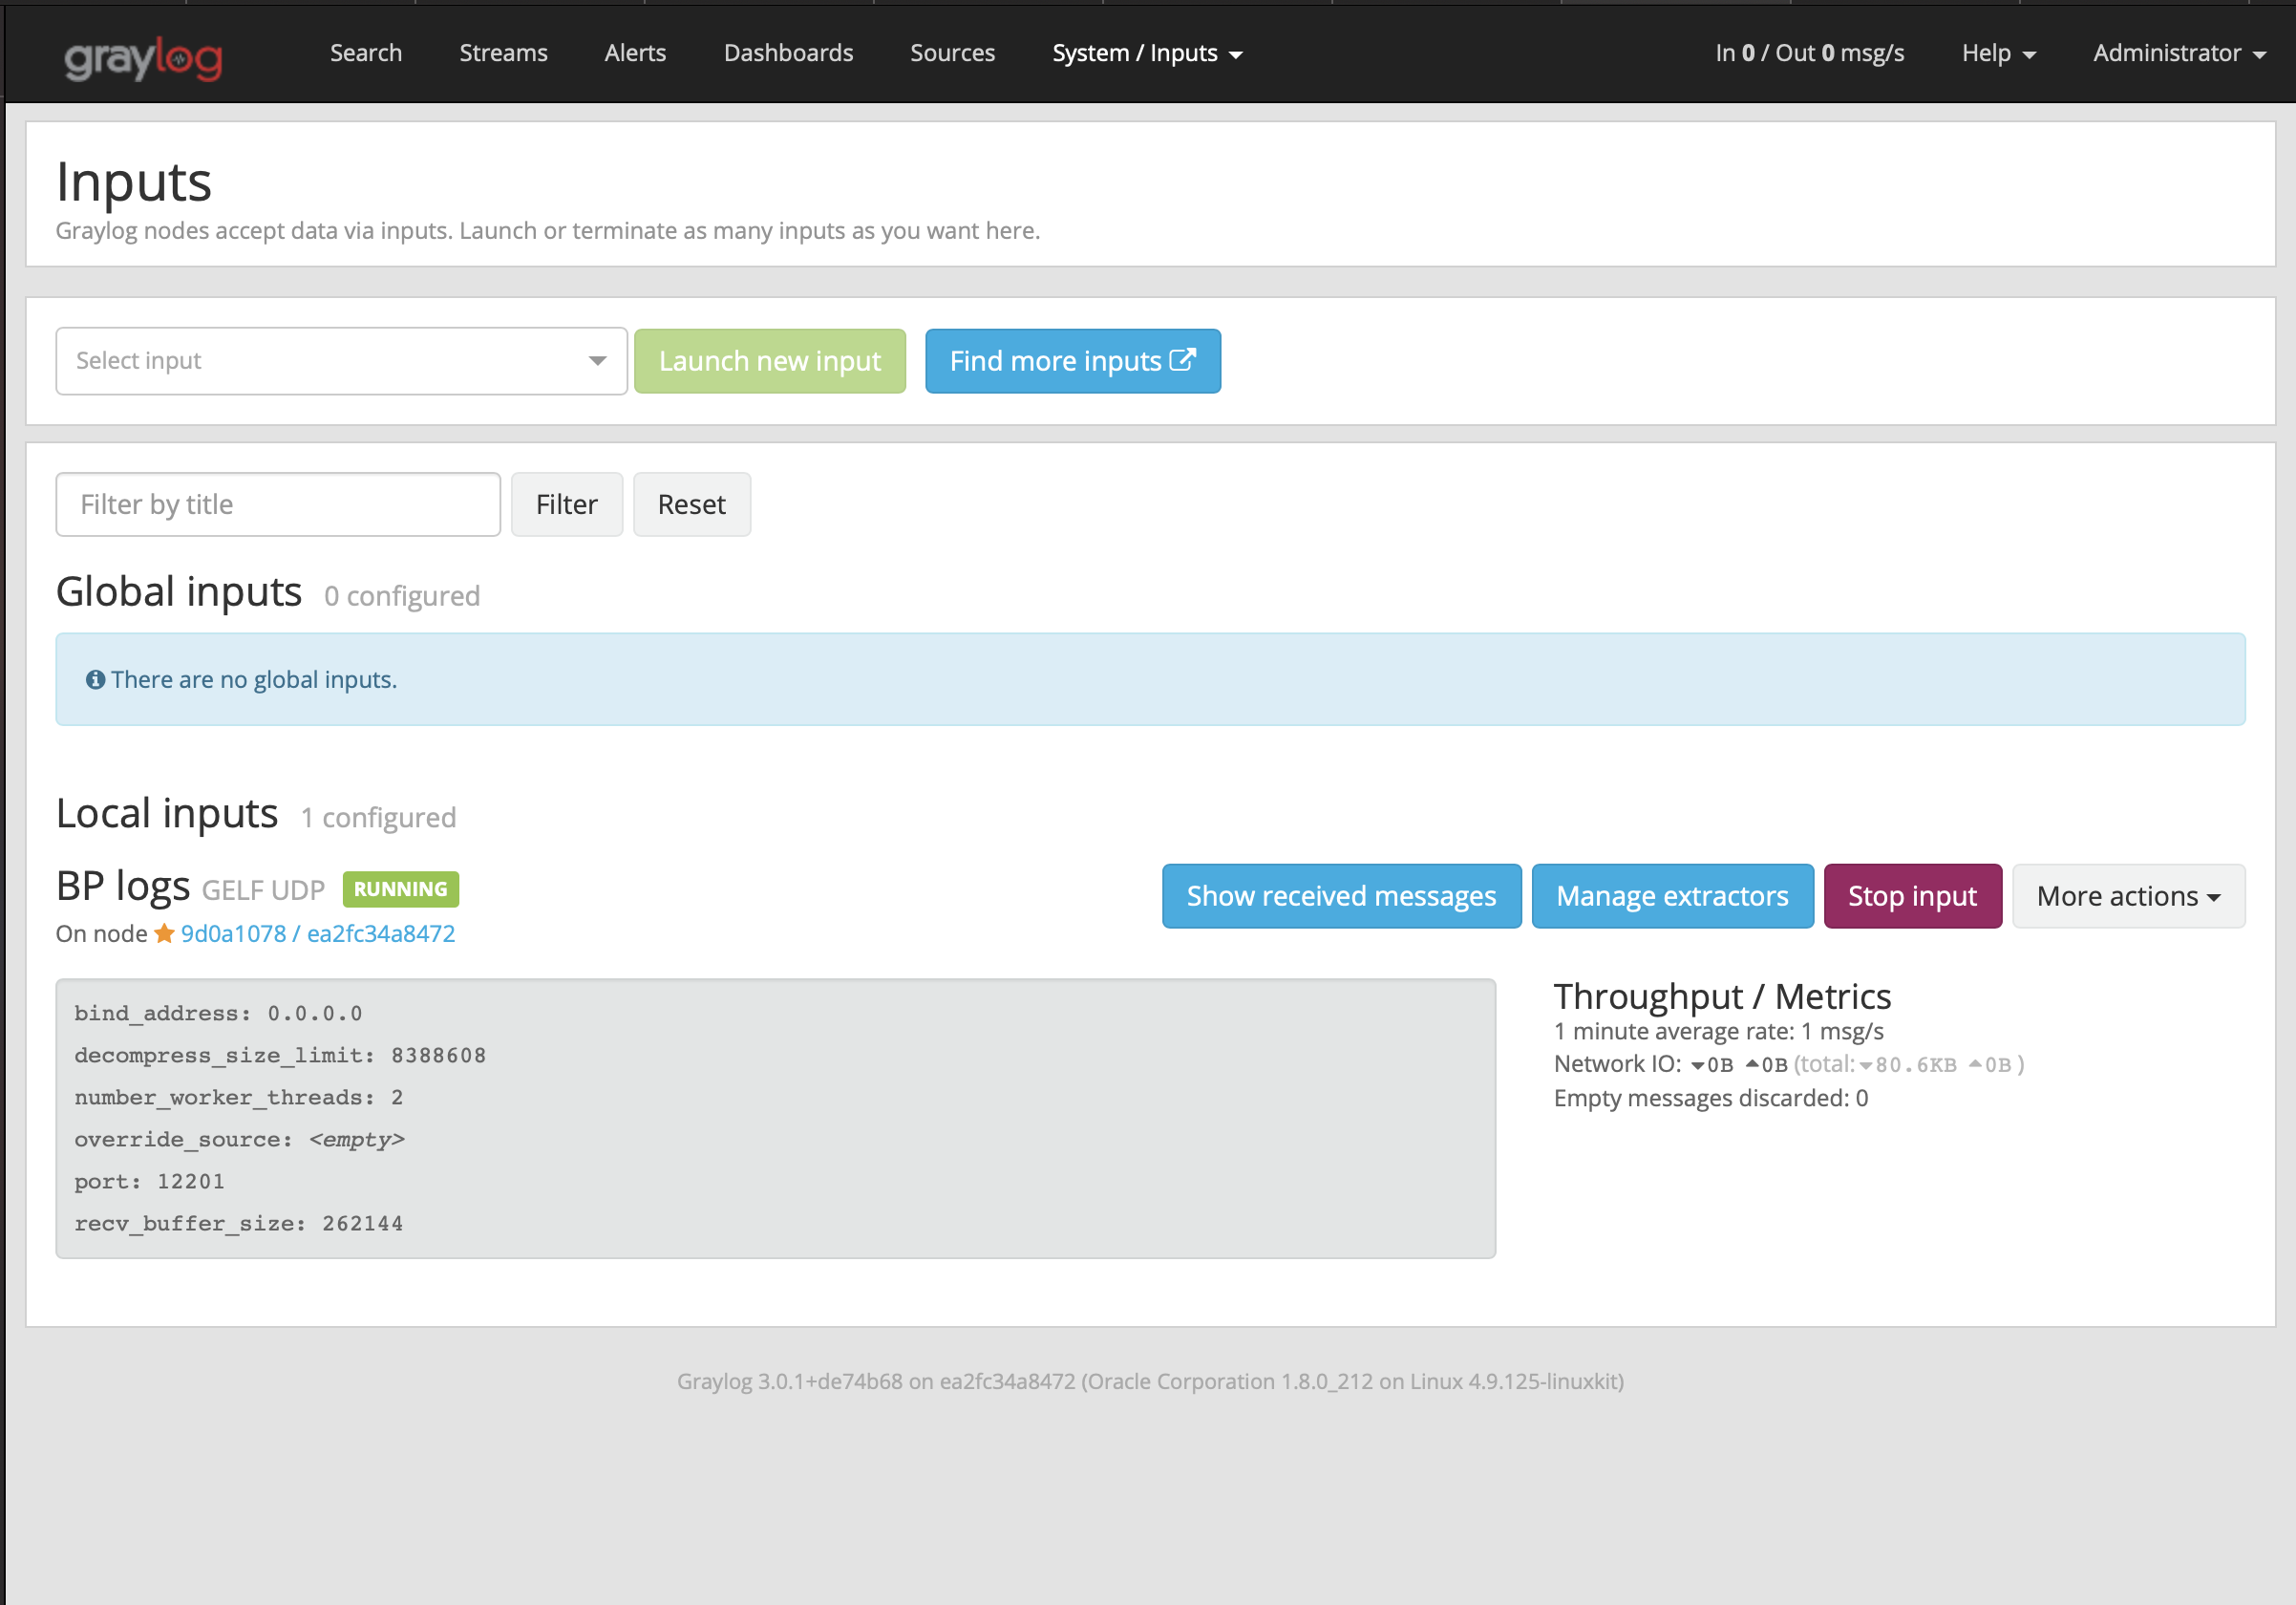
\includegraphics[scale=0.35]{img/graylog_input}
    \caption[Graylog input sherm]{Graylog input scherm}
\end{figure}

\subsection{Kubernetes omgeving}
Graylog configureren voor een Kubernetes omgeving is geen eenvoudige taak. Er wordt best gebruik gemaakt van github repositories om deze aan te passen naar eigen use case. Een dieper inzicht in deze complexe configuratie is overbodig in dit onderzoek en zal dus overgeslagen worden.

\section{Requirements}

\subsection{Must have}
\subsubsection{Moet open source zijn}
Voor elk van de onderzochte oplossingen geldt dezelfde score voor deze requirement, namelijk 5. Graylog is open source en kan vrij gebruikt worden op eigen servers.

\subsubsection{Ondersteuning voor cluster omgevingen zoals Kubernetes}
Zoals reeds vermeld in ~\ref{subsec:graylog} zorgt de ouderdom van deze oplossing ervoor dat deze niet geoptimaliseerd is voor een gedistribueerde omgeving. Graylog heeft wel al een oplossing aangeboden waardoor het mogelijk wordt om de oplossing in een Kubernetes cluster te plaatsen. 

Om deze reden krijgt Graylog een score van 2 op dit requirement.

\subsubsection{Moet een zo klein mogelijke impact hebben op de servers}
Voor Graylog geldt een zelfde uitleg als de ELK of Elastic stack voor dit requirement. Het maakt gebruik van Elasticsearch voor de opslag van logs. Het verschil hierin is dat Graylog gebruik maakt van een eigen log format GELF waardoor de opslag ervan geoptimaliseerd wordt \autocite{graylogdocs}.

Om deze reden krijgt Graylog een score van 3 op dit requirement.

\subsubsection{Moet kunnen scalen naargelang de groeiende Kubernetes cluster}
Het is mogelijk om Graylog mee te scalen met een groeiende cluster. Dit vergt echter wel de toevoeging van Fluentbit of Fluentd als een DaemonSet. Dit zorgt voor extra configuratie waar in een latere requirement rekening mee gehouden moet worden.

Om deze reden krijgt Graylog een score van 3 op dit requirement.

\subsection{Should have}
\subsubsection{Moet (relatief) eenvoudig te configureren zijn}
Zoals hierboven bij de requirement `Moet kunnen scalen naargelang de groeiende Kubernetes cluster`reeds vermeld werd, zorgt de toevoeging van Fluentbit of Fluentd voor extra configuratie. Dit komt bovenop de configuratie van Elasticsearch, Graylog zelf, en MongoDB voor het opslaan van de metadata. 
De configuratie van Elasticsearch is hetzelfde als reeds besproken in Hoofdstuk~\ref{ch:EFK} EFK. 

Om deze redenen krijgt Graylog een score van 2 op dit requirement.

\subsubsection{Moet (relatief) eenvoudig te gebruiken zijn}
Na de installatie is het moeilijkste achter de rug. De Graylog front end webservice beschikt over een soortgelijke functionaliteit als Kibana bij de ELK en EFK stacks. Bijgevolg kan een soortgelijk score gegeven worden aan Graylog, namelijk 4.

\subsubsection{Moet goed gedocumenteerd zijn}
De maturiteit van Graylog zorgt voor een overvloed aan documentatie voor het opstellen van Graylog in bijna elk soort omgeving, behalve Kubernetes. Aangezien de ondersteuning hiervoor nog steeds minimaal is, kan hetzelfde gezegd worden over de documentatie omtrent een Kubenernetes omgeving.

Omdat in het kader van dit onderzoek enkel gekeken wordt naar de documentatie omtrent Kubernetes deployment krijgt Graylog een score van 2 op dit requirement.

\subsubsection{Moet de logs overzichtelijk kunnen tonen}
De Graylog front end webservice beschikt over een soortgelijke functionaliteit als Kibana bij de ELK en EFK stacks. Hoewel de interface anders is opgebouwd dan die van Kibana kan dezelfde score gegeven worden aan elk van deze drie oplossingen, namelijk 5.

\subsubsection{Ondersteuning voor verschillende plugins die data extra kunnen verwerken of naar meerdere locaties kunnen doorsturen}
Dankzij de maturiteit van Graylog is er een grote hoeveelheid diverse plugins beschikbaar. Er is ook veel documentatie beschikbaar voor elke plugin en de manier waarop plugins in het algemeen gebruikt worden.

Om deze reden krijgt Graylog een score van 4 op dit requirement.

\subsubsection{Ondersteuning voor visualisatie zoals grafieken}
Voor Graylog geldt een zelfde uitleg als de ELK of Elastic stack voor dit requirement. Aangezien de de front end web service van Graylog en Kibana zo soortgelijk zijn, krijgen deze beiden dezelfde score, namelijk 5.

\subsection{Could have}
\subsubsection{Ondersteuning voor alerts}
Voor Graylog geldt een zelfde uitleg als de ELK of Elastic stack voor dit requirement. Aangezien de de front end web service van Graylog en Kibana zo soortgelijk zijn, krijgen deze beiden dezelfde score, namelijk 5.

\section{Resultaten}

Wanneer enkel gekeken wordt naar de eerste kolom met de scores op 5 is te zien dat Graylog slecht scoort op belangrijke requirements zoals ondersteuning voor cluster omgevingen, configuratie, en documentatie. De frontend van Graylog scoort dan weer goed met de overzichtelijkheid ervan. Wanneer de belangrijkheidsgraad in rekening wordt gebracht valt meteen op dat Graylog veel minder geschikt is voor de besproken use case dan de andere oplossingen. Een uitgebreide conclusie is te vinden in Hoofdstuk~\ref{ch:conclusie} Conclusie.

\begin{table}[]
    \begin{tabular}{| m{20em} | m{2cm} | m{2cm} | m{2cm} | }
        \hline
        \textbf{Requirement}                                                                                              & \textbf{Score (op 5)} & \textbf{Multiplier} & \textbf{Score met multiplier} \\ \hline
        Moet open source zijn                                                                                             & 5                     & 10                  & 50                            \\ \hline
        Ondersteuning voor cluster omgevingen zoals Kubernetes                                                            & 2                     & 10                  & 20                            \\ \hline
        Moet een zo klein mogelijke impact hebben op de servers                                                           & 3                     & 10                  & 30                            \\ \hline
        Moet kunnen scalen naargelang de groeiende Kubernetes cluster                                                     & 3                     & 10                  & 30                            \\ \hline
        Moet (relatief) eenvoudig te configureren zijn                                                                    & 2                     & 5                   & 10                            \\ \hline
        Moet (relatief) eenvoudig te gebruiken zijn                                                                       & 4                     & 5                   & 20                            \\ \hline
        Moet goed gedocumenteerd zijn                                                                                     & 2                     & 5                   & 10                            \\ \hline
        Moet de logs overzichtelijk kunnen tonen                                                                          & 5                     & 5                   & 25                            \\ \hline
        Ondersteuning voor verschillende plugins die data extra kunnen verwerken of naar meerdere locaties kan doorsturen & 4                     & 5                   & 20                            \\ \hline
        Ondersteuning voor visualisatie zoals grafieken                                                                   & 5                     & 5                   & 25                            \\ \hline
        Ondersteuning voor alerts                                                                                         & 5                     & 1                   & 5                             \\ \hline
        \textbf{Totale score}                                                                                             & 40                    &                     & 245                           \\ \hline
    \end{tabular}
    \caption{Graylog resultaten}
    \label{tab:graylog-resultaten}
\end{table}
%%=============================================================================
%% Loki
%%=============================================================================

\chapter{Loki}
\label{ch:loki}

\section{Installatie en configuratie}

\subsection{Lokale omgeving}
De lokale installatie van de Loki stack kan volledig overgenomen worden van de officiële documentatie van Loki die te vinden is op github.com/grafana/loki. Er zijn 3 belangrijke stappen bij installeren van deze stack. 
\begin{enumerate}
    \item Promtail zoekt de log files in de locaties die gespecifieerd worden in de configuratie (zie listing 7.1). Daarna stuurt deze ze door naar Loki waar ze opgeslagen worden.
    \item Loki slaat de logs die via de gespecifieerde poort binnenkomen via Promtail.
    \item Grafana is de frontend van deze stack, hier worden de eerste 1000 logs van Loki binnengehaald en overzichtelijk gepresenteerd.
\end{enumerate}

Grafana biedt ook een gratis cloud hosted oplossing aan voor test doeleinden. Indien gebruik gemaakt wordt van deze oplossing moet enkel promtail geconfigureerd worden. Documentatie hiervoor is te vinden op de documentatie pagina van Grafana.

\subsubsection{Promtail}
De belangrijkste configuratie punten van de configuratie in Listing 7.1 worden hier besproken.

Een eerste belangrijk configuratie punt is de client url. Deze definieert waar de gevonden logs naartoe worden gestuurd. Bij de lokale configuratie zal dit altijd localhost zijn. De poort 3100 die in Listing 7.1 gedefineerd staat, is terug te vinden in Listing 7.2 als de poort van Loki waarop geluisterd wordt naar binnenkomende calls.

Een tweede belangrijk configuratie punt is de scrapeconfigs. Deze definieert alles van het scrapen logs. In zijn simpelste vorm, zoals te zien is in Listing 7.1, gaat het slechts om 1 job die op zoek gaat naar logs in slechts 1 locatie. Deze configuratie kan snel ingewikkeld worden wanneer sprake is van meerdere jobs die elk meerdere locaties in de gaten houden. Elke locatie heeft zijn eigen label. Zo worden de logs in Grafana makkelijker gefilterd en zullen deze overzichtelijker te tonen zijn. Een andere manier om de configuratie ingewikkelder te maken is het blacklisten van sommige locaties. Dit wil zeggen dat sommige locaties genegeerd worden terwijl andere wel gescrapet worden. Extra informatie over de volledige configuratiemogelijkheden zijn te vinden op github.com/grafana/loki.

Deze configuratie wordt op zijn beurt gebruikt binnen docker container die te vinden is in de officiële docker hub repositories van Grafana, namelijk hub.docker.com/u/grafana. Bij het aanmaken van deze container moet ook een volume gespecifieerd worden. Dit volume is een locatie in de lokale omgeving die gekoppeld wordt met de container. Het commando in dit voorbeeld is te zien op Listing 7.2.

\begin{lstlisting}[caption=promtail-config yaml file ]
server:
    http_listen_port: 9080
    grpc_listen_port: 0

positions:
    filename: /tmp/positions.yaml

client:
    url: http://localhost:3100/api/prom/push

scrape_configs:
    - job_name: log-test
        entry_parser: raw
        static_configs:
        - targets:
            - localhost
        labels:
            job: bp
            __path__: /etc/promtail/logs/*.log  
\end{lstlisting}

\begin{lstlisting}[caption=Aanmaken van de promtail container]
$ docker run --name promtail --volume "$PWD:/etc/promtail" grafana/promtail:master -config.file=/etc/promtail/config.yaml
\end{lstlisting}

\subsubsection{Loki}

De belangrijkste configuratie punten van de configuratie in Listing 7.3 worden hier besproken.

Een eerste belangrijk configuratiepunt is de http listen port. Zoals reeds vermeld in de subsectie Promtail hierboven is dit de poort waar Loki naar luistert en Promtail logs naar stuurt. 

Een tweede belangrijk configuratiepunt is de ingester. De functie hiervan werd reeds besproken in de literatuurstudie van dit werk. 

Een derde belangrijk configuratiepunt is de schema config. Deze definieert de databanken waar de chunks en indexen opgeslagen worden. De chunks worden in een objectstore opgeslagen. In een basis lokale configuratie zal dit het filesystem zijn zoals in Listing 7.3 maar er zijn reeds andere object store databanken ondersteund door Grafana. Voorbeelden hiervan zijn Google Cloud en AWS S3. De indexen worden opgeslagen in een NoSQL databank. Standaard staat deze ingesteld op boltdb, wat een lokale NoSQL databank is. Ook deze databank kan veranderd worden door een gewenste databank.

Een laatste belangrijk punt in de configuratie van Loki is de storage config. Zoals hierboven reeds vermeld worden de indexen en chunks opgeslagen in respectievelijk een NoSQL databank en een Object Store. De locatie hiervan wordt in deze configuratie gespecifieerd.

Deze configuratie wordt op zijn beurt gebruikt binnen docker container die te vinden is in de officiële docker hub repositories van Grafana, namelijk hub.docker.com/u/grafana. Het commando in dit voorbeeld is te zien op Listing 7.2.

\begin{lstlisting}[caption=Loki config yaml file]
auth_enabled: false

server:
    http_listen_port: 3100

ingester:
    lifecycler:
        address: 127.0.0.1
        ring:
            store: inmemory
            replication_factor: 1
        chunk_idle_period: 15m

schema_config:
    configs:
        - from: 0
            store: boltdb
            object_store: filesystem
            schema: v9
            index:
                prefix: index_
                period: 168h

storage_config:
    boltdb:
        directory: /tmp/loki/index

    filesystem:
        directory: /tmp/loki/chunks

limits_config:
    enforce_metric_name: false
\end{lstlisting}

\begin{lstlisting}[caption=Aanmaken van Loki container]
$ docker run --name loki grafana/loki:latest -config.file=/etc/loki/local-config.yaml
\end{lstlisting}

\subsubsection{Grafana}

Om Grafana lokaal te hosten wordt gebruik gemaakt van Homebrew voor Mac OS. Met twee simpele commando's, Listing 7.5 en Listing 7.6 wordt Grafana opgestart op de standaard poort, namelijk 3000.

De volgende stap is Loki linken met Grafana. Dit gebeurt door Loki als datasource te selecteren in de Grafana UI. Daarna zijn de logs te zien in het Explore tab van de UI. Nu is het mogelijk om logs te filteren en te queriën op label of job zoals te zien is in Afbeelding 7.1.

\begin{lstlisting}[language=bash, caption=install grafana]
$ brew install grafana
\end{lstlisting}
\begin{lstlisting}[language=bash, caption=start grafana]
$ brew services start grafana
\end{lstlisting}

\begin{figure}[ht]
    \centering
    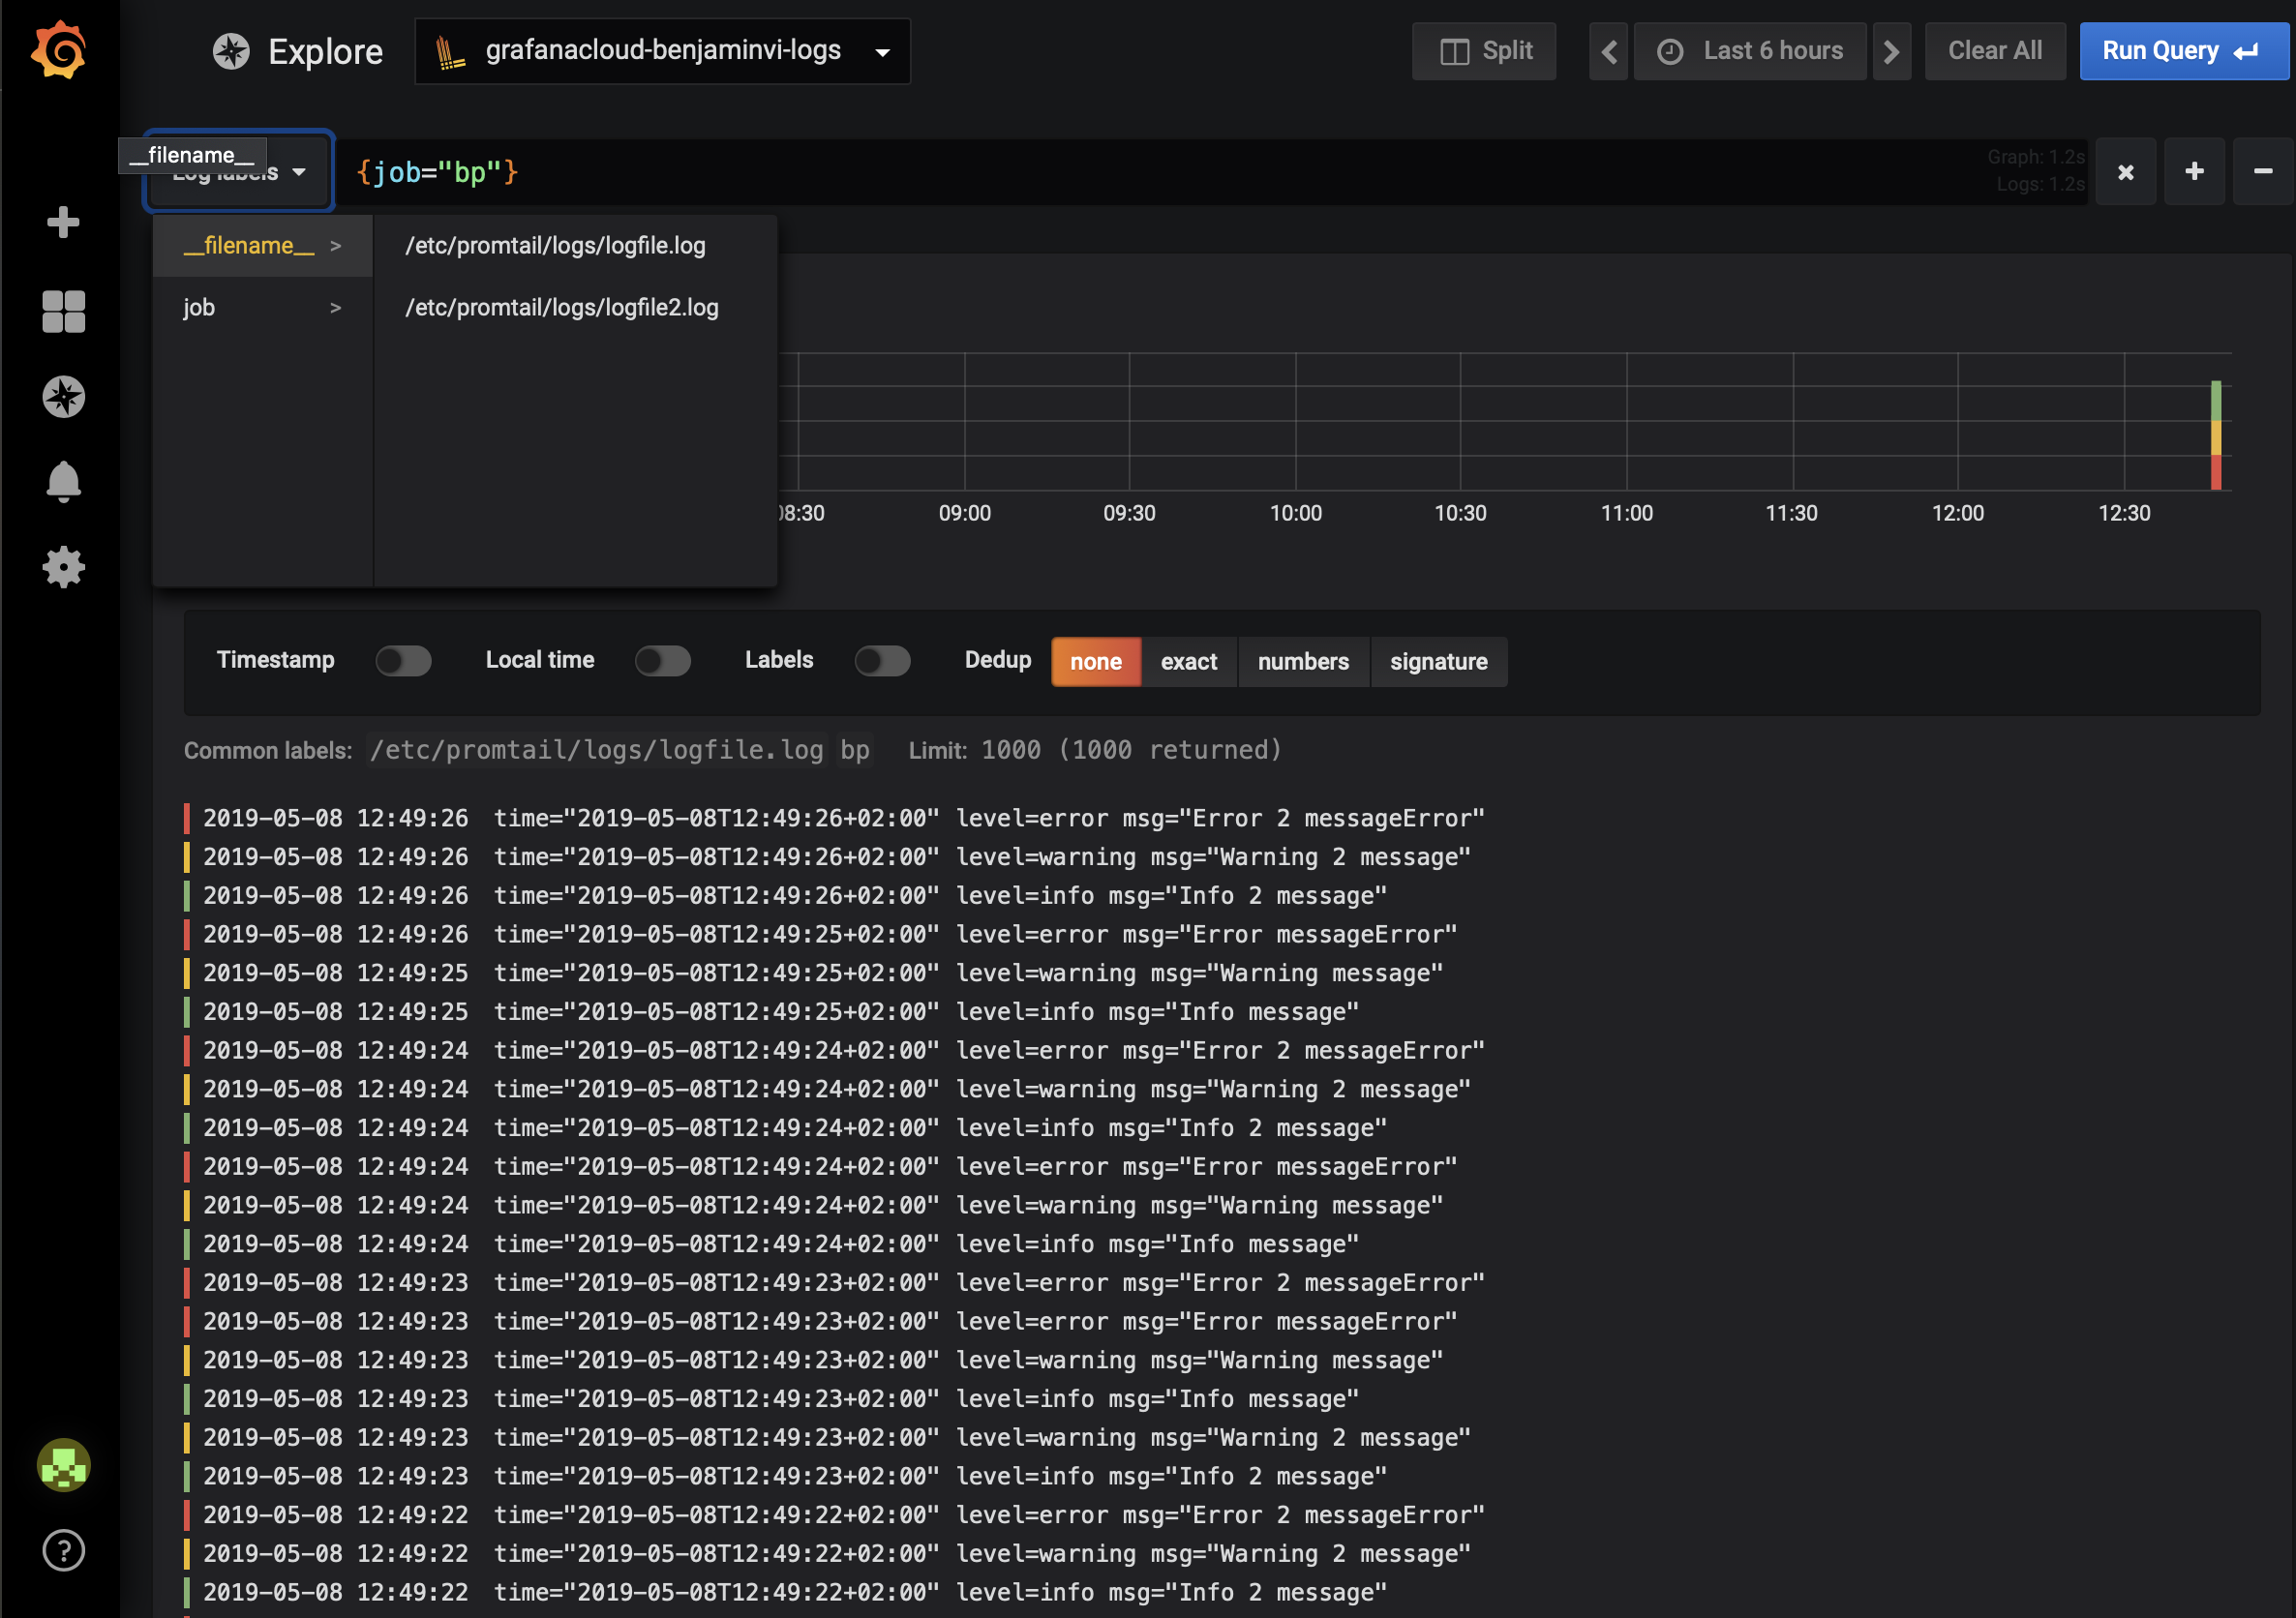
\includegraphics[scale=0.35]{img/loki_query}
    \caption[Loki query]{Loki query}
\end{figure}


\subsection{Kubernetes omgeving}

De Kubernetes deployment van deze oplossing is relatief eenvoudig. Grafana ondersteund nog geen dashboards en alerts voor een Loki datasource, daarom is het niet nodig om services hiervoor te deployen. Grafana kan simpelweg deployed worden op Kubernetes met de out-of-the-box docker image die te vinden is op de docker hub repository van Grafana. In Listing 7.7 wordt het commando hiervoor getoond. Om de Grafana UI te bereiken moet de Kubernetes poort hiervan nog geforward worden naar een eigen poort naar keuze. Dit gebeurt door gebruik te maken van het commando in Listing 7.8\\

\begin{lstlisting}[caption=Grafana Kubernetes deployment]
$kubectl create deployment grafana --image=docker.io/grafana/grafana:latest
\end{lstlisting}
\begin{lstlisting}[caption=Port-forwarding van Grafana]
$kubectl port-forward service/loki-grafana 3000:80
\end{lstlisting}

De andere componenten Promtail en Loki zijn te installeren via Helm charts die beschikbaar zijn in de github pagina van Grafana, namelijk github.com/grafana/loki/tree/master/production. Door gebrek aan documentatie valt hier geen extra uitleg bij te geven over de exacte configuratie die gebruikt wordt in deze Helm charts.


\section{Requirements}

\subsection{Must have}
\subsubsection{Moet open source zijn}
Voor elk van de onderzochte oplossingen geldt dezelfde score voor deze requirement, namelijk 5. Elk van de componenten waaruit een Loki `stack` bestaat, namelijk Promtail, Loki, en Grafana, is vrij te verkrijgen en te gebruiken.

\subsubsection{Ondersteuning voor cluster omgevingen zoals Kubernetes}
Loki is speciaal voor Kubernetes ontwikkeld. Deze oplossing kan ook buiten Kubernetes gebruikt worden maar werkt het best in een Kubernetes cluster. 

Om deze reden krijgt Loki een score van 5 op dit requirement.

\subsubsection{Moet een zo klein mogelijke impact hebben op de servers}
Loki heeft een minimale impact op de servers. Waar Elasticsearch gebruik maakt van volledige indexering bij het opslaan van logs, indexeert Loki enkel de metadata van logs waardoor het opslagverbruik lager ligt. Verder is ook nagedacht over de manier van het opslaan. De indexen worden opgeslagen in een object store. De logs worden via een distributor ondergebracht in ingestors. Deze worden gevuld met soortgelijke logs en worden opgeslagen in een NoSQL databank eens deze opgevuld zijn.

Om deze redenen krijgt Loki een score van 5 op dit requirement.

\subsubsection{Moet kunnen scalen naargelang de groeiende Kubernetes cluster}
Promtail, de log scraper van Loki, kan ook geconfigureerd worden als een DaemonSet waardoor automatische scaling gegarandeerd kan worden. 

Om deze reden krijgt Loki een score van 5 op dit requirement.

\subsection{Should have}
\subsubsection{Moet (relatief) eenvoudig te configureren zijn}
In het requirement `Moet goed gedocumenteerd zijn` hieronder zal nog verder uitgelegd worden waarom er weinig documentatie beschikbaar is. Het gebrek aan documentatie leidt tot een moeilijke configuratie voor een nieuwe gebruiker. Elk van de component zijn relatief eenvoudig te configureren eens wat meer ervaring is opgedaan.

Om deze redenen krijgt Loki een score van 3 op dit requirement.

\subsubsection{Moet (relatief) eenvoudig te gebruiken zijn}
Het gebruiksgemak van Loki wordt meteen duidelijk na de installatie en configuratie. Het overzicht van de logs en de manier waarop logs worden opgeslagen met labels  zorgen voor een aangename gebruikerservaring.

Om deze reden krijgt Loki een score van 5 op dit requirement.

\subsubsection{Moet goed gedocumenteerd zijn}
De documentatie van Loki is op het moment van schrijven quasi onbestaand. Buiten de officiële documentatie van Grafana zijn er slechts enkele bronnen beschikbaar. Dit is voornamelijk te wijten aan het feit dat Loki nog in een beta fase zit. Deze oplossing is nog niet zo lang geleden uitgekomen en wordt nog volop ontwikkeld. 

Om deze reden krijgt Loki een score van 2 op dit requirement.

\subsubsection{Moet de logs overzichtelijk kunnen tonen}
Grafana maakt gebruik van een eigen interface om de logs te tonen. Deze worden in een lijst van 1000 onder elkaar geplaatsd. Wanneer specifiek op zoek moet worden gegaan is er de mogelijk op te zoeken op labels en zo de getoonde lijst te verfijen. De query taal om logs te filteren is nog onder constructie waardoor de functionaliteit op dit moment vrij beperkt is. Dit is een belangrijke factor in de score van dit requirement

Om deze reden krijgt Loki een score van 2 op dit requirement.

\subsubsection{Ondersteuning voor verschillende plugins die data extra kunnen verwerken of naar meerdere locaties kunnen doorsturen}
Er zijn niet veel plugins beschikbaar die een soortgelijke functionaliteit hebben als beschreven in de requirement. Maar dit probleem is makkelijk op te lossen met het implementeren van Fluentd als log collector. Met deze configuratie scrapet Promtail al pod logs naar Fluentd. Deze verwerkt de logs en kan gebruik maken van een grote hoeveelheid plugins hiervoor. Na de verwerking worden de logs dan doorgestuurd naar Loki waar ze opgeslagen worden.

Om deze reden krijgt Loki een score van 4 op dit requirement.

\subsubsection{Ondersteuning voor visualisatie zoals grafieken}
Grafana heeft reeds ondersteuning voor grafieken en dergelijke voor het visualiseren van verschillende databronnen. Momenteel is Grafana ondersteuning voor een Loki databron aan het toevoegen voor dit onderdeel en zal ook aan deze requirement voldaan worden. Aangezien dit nog niet het geval is krijgt Loki een score van 1 voor deze requirement.

\subsection{Could have}
\subsubsection{Ondersteuning voor alerts}
Grafana heeft reeds ondersteuning voor alerts voor verschillende databronnen. Momenteel is Grafana ondersteuning voor een Loki databron aan het toevoegen voor dit onderdeel en zal ook aan deze requirement voldaan worden. Aangezien dit nog niet het geval is krijgt Loki een score van 1 voor deze requirement.

\section{Resultaten}
Zoals te zien is in tabel~\ref{tab:Loki-resultaten}, scoort Loki in eerste instantie niet zo hoog bij een standaard score op 5. Wanneer deze score wordt verwerkt aan de hand van belangrijkheidsgraad, is te zien dat Loki wel degelijk veel potentieel biedt. De score is gebaseerd op hoe Loki functioneert op het moment van schrijven van dit werk. Het product heeft nog een lange weg te gaan maar heeft reeds een perfecte score op de vier Must Have requirements. Mits wat verbeteringen op vlak van documentatie en visualisatie zal de score van Loki nog verbeteren.

Een uitgebreide conclusie is te vinden in Hoofdstuk~\ref{ch:conclusie} Conclusie.
\begin{table}[]
    \begin{tabular}{| m{20em} | m{2cm} | m{2cm} | m{2cm} | }
        \hline
        \textbf{Requirement}                                                                                              & \textbf{Score (op 5)} & \textbf{Multiplier} & \textbf{Score met multiplier} \\ \hline
        Moet open source zijn                                                                                             & 5                     & 10                  & 50                            \\ \hline
        Ondersteuning voor cluster omgevingen zoals Kubernetes                                                            & 5                     & 10                  & 50                            \\ \hline
        Moet een zo klein mogelijke impact hebben op de servers                                                           & 5                     & 10                  & 50                            \\ \hline
        Moet kunnen scalen naargelang de groeiende Kubernetes cluster                                                     & 5                     & 10                  & 50                            \\ \hline
        Moet (relatief) eenvoudig te configureren zijn                                                                    & 3                     & 5                   & 15                            \\ \hline
        Moet (relatief) eenvoudig te gebruiken zijn                                                                       & 5                     & 5                   & 25                            \\ \hline
        Moet goed gedocumenteerd zijn                                                                                     & 2                     & 5                   & 10                            \\ \hline
        Moet de logs overzichtelijk kunnen tonen                                                                          & 2                     & 5                   & 10                            \\ \hline
        Ondersteuning voor verschillende plugins die data extra kunnen verwerken of naar meerdere locaties kan doorsturen & 5                     & 5                   & 25                            \\ \hline
        Ondersteuning voor visualisatie zoals grafieken                                                                   & 1                     & 5                   & 5                             \\ \hline
        Ondersteuning voor alerts                                                                                         & 1                     & 1                   & 1                             \\ \hline
        \textbf{Totale score}                                                                                             & 39                    &                     & 291                           \\ \hline
    \end{tabular}
    \caption{Loki resultaten}
    \label{tab:Loki-resultaten}
\end{table}

% Voeg hier je eigen hoofdstukken toe die de ``corpus'' van je bachelorproef
% vormen. De structuur en titels hangen af van je eigen onderzoek. Je kan bv.
% elke fase in je onderzoek in een apart hoofdstuk bespreken.

%\input{...}
%\input{...}
%...

%%=============================================================================
%% Conclusie
%%=============================================================================

\chapter{Conclusie}
\label{ch:conclusie}

%% TODO: Trek een duidelijke conclusie, in de vorm van een antwoord op de
%% onderzoeksvra(a)g(en). Wat was jouw bijdrage aan het onderzoeksdomein en
%% hoe biedt dit meerwaarde aan het vakgebied/doelgroep? Reflecteer kritisch
%% over het resultaat. Had je deze uitkomst verwacht? Zijn er zaken die nog
%% niet duidelijk zijn? Heeft het onderzoek geleid tot nieuwe vragen die
%% uitnodigen tot verder onderzoek?


In dit onderzoek wordt een antwoord gegeven op de onderzoeksvraag `Wat is de beste open-source logging met tracing oplossing voor een bedrijf als Be-Mobile?`. Om dit te onderzoeken is een vergelijkende studie uitgevoerd tussen de meest voornaamste vier logging oplossingen, namelijk de Elastic stack, de ELK stack, Graylog, en Grafana Loki. Er werd gekeken naar enkele kernelementen van een goede logging oplossing en elk van de onderzochte oplossingen werd hieraan getoetst.

Als eerste conclusie kan gesteld worden dat logging en tracing verschillende onderwerpen zijn. Tracing werd ook onderzocht in dit werk en hoewel dit onderzoek zeer nuttig is geweest voor Be-Mobile is er besloten om de uitwerking hiervan niet op te nemen in dit werk.

Een tweede conclusie is dat er geen enkele oplossing voldoet aan de eisen die in het begin van dit onderzoek gesteld werden. EFK en ELK scoren uitstekend op visualisatie en documentatie, maar door de overhead die gepaard gaat met Elasticsearch zijn deze minder geschikte oplossingen. De complexiteit van de manier waarop Elasticsearch geconfigureerd moet worden in een Kubernetes cluster speelt hier een grote rol. Loki daarentegen zorgt voor een minimale overhead dankzij de architectuur ervan en biedt veel mogelijkheden. Het nadeel aan Loki is dat ontwikkeling ervan zich nog steeds in een beta fase bevindt. Dit leidt tot een gebrek aan documentatie en slechts een minimale ondersteuning in Grafana. Ondanks de jeugdigheid van Loki, kan het nu al aanschouwt worden als de meest geschikte oplossing in een microservice omgeving met een hoog aantal nodes. Waar EFK, ELK, en Graylog reeds volledig ontwikkeld zijn en dus vastzitten aan de manier waarop ze zijn opgebouwd, is Loki nog volop in ontwikkeling en bezit het dus veel potentieel om uit te groeien tot de ideale open source logging oplossing op de markt.

Een derde conclusie die kan getrokken worden uit dit onderzoek is dat elk van de onderzochte oplossingen beter gehost wordt door de service die de deze ontwikkeld heeft. De kost die gepaard gaat met de uitbreiding van een Kubernetes cluster zal op een gegeven moment de kost van hosting voorbij gaan. Het nadeel aan deze aanpak is het verlies van controle over de cluster. Hoewel dit zeker geen oplossing is in het geval van Be-Mobile, kan dit zeker een optie zijn voor een ander bedrijf die dit werkt leest.

Concreet kan gesteld worden dat de EFK stack de voordeligste optie is wanneer Elasticsearch wordt gebruikt. Loki is de oplossing met het meeste potentieel. De keuze hiertussen moet gemaakt worden op basis van budget. Wanneer beschikt wordt over een groot budget, zal EFK de meest geschikte oplossing zijn. Indien hier absoluut geen budget voor beschikbaar is, moet geïnvesteerd worden in de toekomst met Loki als meest geschikte oplosssing.

Deze conclusies waren volledig onverwacht. Zoals te zien is in het onderzoeksvoorstel van dit werk, is te zien dat oorspronkelijk tracing verwerkt was in dit werk. Ook werd verwacht dat op zoek zou gegaan worden naar een databank en logging framework, niet naar een volledige oplossing. Bij aanvang van het onderzoek zelf werd snel duidelijk dat het werk zou gaan over de verschillende logging oplossingen. Zelfs op dat moment werden zulke conclusies niet verwacht. 

Wegens de nogal opiniegerichte wijze van vergelijken in dit werk, wordt de nood aan een nieuw onderzoek duidelijk. Dit zou dieper ingaan op de impact op het systeem van elke oplossing. Een simulatie van een soortgelijke omgeving als bij Be-Mobile is hiervoor vereist. Deze vergelijking zou in een latere fase nogmaals uitgevoerd kunnen worden, dit wanneer Loki al wat verder ontwikkeld werd. De verwachte conclusie voor die vergelijking zou dan zeker in het verdeel van Loki zijn.

Dit werk kan als nuttig beschouwd worden door bedrijven of startups die op zoek zijn naar een logging backend voor hun microservices. De requirement `Moet kunnen scalen naargelang de groeiende Kubernetes cluster` is een belangrijke requirement voor een zulke doelgroep. Ook personen die interesse in microservices of logging in het algemeen kunnen dit werk gebruiken als basis om een diepere kennis te vergaren in het onderwerp.

%%=============================================================================
%% Bijlagen
%%=============================================================================

\appendix

%%---------- Onderzoeksvoorstel -----------------------------------------------

\chapter{Onderzoeksvoorstel}

Het onderwerp van deze bachelorproef is gebaseerd op een onderzoeksvoorstel dat vooraf werd beoordeeld door de promotor. Dat voorstel is opgenomen in deze bijlage.

% Verwijzing naar het bestand met de inhoud van het onderzoeksvoorstel
%---------- Inleiding ---------------------------------------------------------

\section{Introductie} % The \section*{} command stops section numbering
\label{sec:introductie}

Hier introduceer je werk. Je hoeft hier nog niet te technisch te gaan.

Je beschrijft zeker:

\begin{itemize}
  \item de probleemstelling en context
  \item de motivatie en relevantie voor het onderzoek
  \item de doelstelling en onderzoeksvraag/-vragen
\end{itemize}

%---------- Stand van zaken ---------------------------------------------------

\section{State-of-the-art}
\label{sec:state-of-the-art}

Hier beschrijf je de \emph{state-of-the-art} rondom je gekozen onderzoeksdomein. Dit kan bijvoorbeeld een literatuurstudie zijn. Je mag de titel van deze sectie ook aanpassen (literatuurstudie, stand van zaken, enz.). Zijn er al gelijkaardige onderzoeken gevoerd? Wat concluderen ze? Wat is het verschil met jouw onderzoek? Wat is de relevantie met jouw onderzoek?

Verwijs bij elke introductie van een term of bewering over het domein naar de vakliteratuur, bijvoorbeeld~\autocite{Doll1954}! Denk zeker goed na welke werken je refereert en waarom.

% Voor literatuurverwijzingen zijn er twee belangrijke commando's:
% \autocite{KEY} => (Auteur, jaartal) Gebruik dit als de naam van de auteur
%   geen onderdeel is van de zin.
% \textcite{KEY} => Auteur (jaartal)  Gebruik dit als de auteursnaam wel een
%   functie heeft in de zin (bv. ``Uit onderzoek door Doll & Hill (1954) bleek
%   ...'')

Je mag gerust gebruik maken van subsecties in dit onderdeel.

%---------- Methodologie ------------------------------------------------------
\section{Methodologie}
\label{sec:methodologie}

Hier beschrijf je hoe je van plan bent het onderzoek te voeren. Welke onderzoekstechniek ga je toepassen om elk van je onderzoeksvragen te beantwoorden? Gebruik je hiervoor experimenten, vragenlijsten, simulaties? Je beschrijft ook al welke tools je denkt hiervoor te gebruiken of te ontwikkelen.

%---------- Verwachte resultaten ----------------------------------------------
\section{Verwachte resultaten}
\label{sec:verwachte_resultaten}

Hier beschrijf je welke resultaten je verwacht. Als je metingen en simulaties uitvoert, kan je hier al mock-ups maken van de grafieken samen met de verwachte conclusies. Benoem zeker al je assen en de stukken van de grafiek die je gaat gebruiken. Dit zorgt ervoor dat je concreet weet hoe je je data gaat moeten structureren.

%---------- Verwachte conclusies ----------------------------------------------
\section{Verwachte conclusies}
\label{sec:verwachte_conclusies}

Hier beschrijf je wat je verwacht uit je onderzoek, met de motivatie waarom. Het is \textbf{niet} erg indien uit je onderzoek andere resultaten en conclusies vloeien dan dat je hier beschrijft: het is dan juist interessant om te onderzoeken waarom jouw hypothesen niet overeenkomen met de resultaten.



%%---------- Andere bijlagen --------------------------------------------------
% TODO: Voeg hier eventuele andere bijlagen toe
%\input{...}

%%---------- Referentielijst --------------------------------------------------

\printbibliography[heading=bibintoc]
%\addcontentsline{toc}{chapter}{\textcolor{maincolor}{\IfLanguageName{dutch}{Bibliografie}{Bibliography}}}

\end{document}
